% !TEX program = xelatex
\documentclass[12pt, a4paper, oneside]{book}
% !TEX root = ../do-an.tex

\usepackage{styles/dau}
\dauLayout

\linespread{1.25}
\usepackage[skip=8pt plus 1pt, indent=15pt]{parskip}



\tikzset{
  sdlbl/.style={font=\tiny, text=daumaroon, fill=white, inner sep=1pt},
  erdt/.style={rectangle, draw=daunavy, line width=0.7pt, fill=white,
               align=left, inner sep=3.5pt, font=\ttfamily\scriptsize,
               text width=34mm},
  erdlink/.style={draw=daumaroon, line width=0.7pt, -{Stealth[length=1.8mm]}},
}

\newcommand{\sodoUseCase}{%
\resizebox{\textwidth}{!}{%
\begin{tikzpicture}[
  act/.style={rectangle, draw=daumaroon, line width=0.9pt, rounded corners=2pt,
              fill=lightwarm, minimum width=2.2cm, minimum height=0.75cm,
              font=\footnotesize\bfseries, text=daumaroon},
  uc/.style={ellipse, draw=daunavy, line width=0.7pt, fill=white,
             minimum width=3.4cm, minimum height=0.72cm,
             font=\scriptsize, align=center, inner sep=1pt},
  ucai/.style={ellipse, draw=daumaroon, line width=1.1pt, fill=lightwarm,
               minimum width=3.4cm, minimum height=0.72cm,
               font=\scriptsize\bfseries, align=center, inner sep=1pt},
  assoc/.style={draw=gray500, line width=0.6pt},
]

  \draw[draw=daunavy, line width=1pt, rounded corners=4pt, fill=gray100]
        (3.0,0.95) rectangle (12.4,-8.65);
  \node[font=\footnotesize\sffamily\bfseries, text=daunavy] at (7.7,0.6)
        {Hệ thống Uni Connect};

  \node[uc]   (uc01) at (5.1,-0.35) {UC-01 Tra cứu điểm chuẩn};
  \node[uc]   (uc02) at (5.1,-1.55) {UC-02 Xem chi tiết trường};
  \node[uc]   (uc03) at (5.1,-2.75) {UC-03 Đăng ký / Đăng nhập};

  \node[uc]   (uc09) at (5.1,-4.85) {UC-09 Cập nhật dữ liệu năm mới};
  \node[ucai] (uc10) at (5.1,-6.05) {UC-10 Huấn luyện lại mô hình $\star$};
  \node[uc]   (uc11) at (5.1,-7.25) {UC-11 Xem thống kê hệ thống};

  \node[uc]   (uc04) at (10.3,-0.35) {UC-04 Nhập hồ sơ năng lực};
  \node[ucai] (uc05) at (10.3,-1.55) {UC-05 Nhận gợi ý (AI) $\star$};
  \node[ucai] (uc06) at (10.3,-2.75) {UC-06 Xem lời giải thích $\star$};
  \node[uc]   (uc07) at (10.3,-3.95) {UC-07 So sánh nguyện vọng};
  \node[uc]   (uc08) at (10.3,-5.15) {UC-08 Lưu / xem lại hồ sơ};

  \node[act] (khach)   at (1.15,-1.55) {Khách};
  \node[act] (quantri) at (1.15,-6.05) {Quản trị viên};
  \node[act] (hocsinh) at (14.55,-2.75) {Học sinh};

  \foreach \u in {uc01, uc02, uc03} \draw[assoc] (khach) -- (\u);
  \foreach \u in {uc09, uc10, uc11} \draw[assoc] (quantri) -- (\u);
  \foreach \u in {uc04, uc05, uc06, uc07, uc08} \draw[assoc] (hocsinh) -- (\u);

  \draw[draw=daumaroon, line width=0.7pt, dashed, -{Stealth[length=1.8mm]}]
        (uc05.east) -- node[sdlbl] {\en{include}} (uc06.east);
  \draw[draw=daumaroon, line width=0.7pt, dashed, -{Stealth[length=1.8mm]}]
        (uc10.west) -- node[sdlbl] {\en{follows}} (uc09.west);

  \node[font=\scriptsize\bfseries, text=daumaroon, align=center] at (7.7,-8.2)
        {$\star$ : Ca sử dụng có mô hình Trí tuệ nhân tạo (Random Forest) tham gia};
\end{tikzpicture}}
}

\newcommand{\sodoBFD}{%
\resizebox{\textwidth}{!}{%
\begin{tikzpicture}[
  root/.style={rectangle, rounded corners=3pt, draw=daumaroon, line width=1.1pt,
               fill=lightwarm, inner sep=5pt, font=\small\bfseries, text=daumaroon,
               align=center, minimum width=17.5cm},
  grp/.style={rectangle, rounded corners=2pt, draw=daumaroon, line width=0.8pt,
              fill=lightwarm, inner sep=4pt, font=\footnotesize\bfseries,
              text=daumaroon, align=center, text width=3.1cm, minimum height=0.85cm},
  fn/.style={rectangle, rounded corners=1.5pt, draw=daunavy, line width=0.5pt,
             fill=white, inner sep=3.5pt, font=\scriptsize, text=daunavy,
             align=left, text width=3.1cm},
  lnk/.style={draw=daumaroon, line width=0.7pt, -{Stealth[length=1.4mm]}}
]
  \node[root] (top) at (8.0, 1.8) {Hệ thống gợi ý nguyện vọng đại học Uni Connect};

  \node[grp] (g1) at (0, 0) {Tra cứu\\(UC-01, 02)};
  \node[grp] (g2) at (4.0, 0) {Tài khoản\\(UC-03)};
  \node[grp] (g3) at (8.0, 0) {Hồ sơ học sinh\\(UC-04, 08)};
  \node[grp] (g4) at (12.0, 0) {Gợi ý AI\\(UC-05, 06, 07)};
  \node[grp] (g5) at (16.0, 0) {Quản trị\\(UC-09, 10, 11)};

  \draw[lnk] (top.south) -| (g1.north);
  \draw[lnk] (top.south) -| (g2.north);
  \draw[lnk] (top.south) -- (g3.north);
  \draw[lnk] (top.south) -| (g4.north);
  \draw[lnk] (top.south) -| (g5.north);

  \node[fn, below=2.5mm of g1] (f11) {$\bullet$~Tìm trường, ngành, tổ hợp, tỉnh};
  \node[fn, below=1.5mm of f11] (f12) {$\bullet$~Lọc vùng miền, phương thức, năm};
  \node[fn, below=1.5mm of f12] (f13) {$\bullet$~Xem chuỗi điểm chuẩn 10 năm};

  \node[fn, below=2.5mm of g2] (f21) {$\bullet$~Đăng ký, đăng nhập nội bộ};
  \node[fn, below=1.5mm of f21] (f22) {$\bullet$~Đăng nhập Google OAuth2};
  \node[fn, below=1.5mm of f22] (f23) {$\bullet$~Đăng nhập Facebook OAuth2};

  \node[fn, below=2.5mm of g3] (f31) {$\bullet$~Nhập điểm thi THPT, học bạ};
  \node[fn, below=1.5mm of f31] (f32) {$\bullet$~Chọn nhóm ngành, vùng quan tâm};
  \node[fn, below=1.5mm of f32] (f33) {$\bullet$~Sửa, xóa, xem danh sách hồ sơ};

  \node[fn, below=2.5mm of g4] (f41) {$\bullet$~Suy luận xác suất đỗ theo lô};
  \node[fn, below=1.5mm of f41] (f42) {$\bullet$~Phân tầng An toàn, Vừa sức, Thử sức};
  \node[fn, below=1.5mm of f42] (f43) {$\bullet$~Sinh lời giải thích từ đặc trưng};
  \node[fn, below=1.5mm of f43] (f44) {$\bullet$~So sánh và lưu nguyện vọng};

  \node[fn, below=2.5mm of g5] (f51) {$\bullet$~Cập nhật điểm chuẩn năm mới};
  \node[fn, below=1.5mm of f51] (f52) {$\bullet$~Trượt cửa sổ 10 năm tự động};
  \node[fn, below=1.5mm of f52] (f53) {$\bullet$~Huấn luyện lại mô hình AI};
  \node[fn, below=1.5mm of f53] (f54) {$\bullet$~Quản lý người dùng, thống kê};
\end{tikzpicture}}
}

\newcommand{\sodoERD}{%
\resizebox{\textwidth}{!}{%
\begin{tikzpicture}

  \node[erdt] (t_truong) at (0,0)
    {{\sffamily\bfseries truong}\\[1pt]
     \textbf{ma\_truong} PK\\ ten\_truong\\ viet\_tat\\ tinh\_thanh\\ vung\_mien};

  \node[erdt, below=5mm of t_truong] (t_nganh)
    {{\sffamily\bfseries nganh}\\[1pt]
     \textbf{nganh\_id} PK\\ nganh\_slug UQ\\ ten\_nganh\\ nhom\_nganh};

  \node[erdt, below=5mm of t_nganh] (t_mon)
    {{\sffamily\bfseries mon}\\[1pt]
     \textbf{ma\_mon} PK\\ ten\_mon\\ la\_nang\_khieu};

  \node[erdt, below=5mm of t_mon] (t_tohop)
    {{\sffamily\bfseries to\_hop}\\[1pt]
     \textbf{ma\_to\_hop} PK\\ ten\_to\_hop\\ cac\_mon};

  \node[erdt, below=5mm of t_tohop] (t_thm)
    {{\sffamily\bfseries to\_hop\_mon}\\[1pt]
     \textbf{ma\_to\_hop} PK, FK\\ \textbf{ma\_mon} PK, FK\\ vi\_tri PK};

  \node[erdt, below=5mm of t_thm] (t_csn)
    {{\sffamily\bfseries cua\_so\_nam}\\[1pt]
     \textbf{vi\_tri} PK\\ nam UQ};

  \node[erdt] (t_dc) at (7.6,0)
    {{\sffamily\bfseries diem\_chuan}\\[1pt]
     \textbf{id} PK\\ ma\_truong FK\\ nganh\_id FK\\ ma\_to\_hop FK\\ phuong\_thuc\\ nam\\ diem\_chuan\\ \textit{uq: 5 cột giữa}};

  \node[erdt, below=5mm of t_dc] (t_dt)
    {{\sffamily\bfseries dac\_trung\_diemchuan}\\[1pt]
     id PK\\ ma\_truong FK\\ nganh\_id FK\\ ma\_to\_hop FK\\ phuong\_thuc\\
     diem\_nam\_1 \dots\ diem\_nam\_10\\
     diem\_tb, diem\_min\\ diem\_max, diem\_moi\_nhat\\
     bien\_dong, xu\_huong\\ so\_nam\_co\_dl};

  \node[erdt, below=5mm of t_dt] (t_lcn)
    {{\sffamily\bfseries lan\_cap\_nhat}\\[1pt]
     id PK\\ thoi\_diem, nguon\\ nam\_bat\_dau\\ nam\_ket\_thuc\\ so\_truong, so\_nganh\\ so\_dong\_diem\\ selfcheck\_dat};

  \node[erdt] (t_user) at (15.2,0)
    {{\sffamily\bfseries auth\_user}\\[1pt]
     \textbf{id} PK\\ username UQ\\ password, email\\ is\_staff\\ is\_active};

  \node[erdt, below=5mm of t_user] (t_hs)
    {{\sffamily\bfseries ho\_so\_nang\_luc}\\[1pt]
     id PK\\ user\_id FK\\ ten\_ho\_so\\ phuong\_thuc\\ diem\_uu\_tien};

  \node[erdt, below=5mm of t_hs] (t_dm)
    {{\sffamily\bfseries diem\_mon}\\[1pt]
     \textbf{ho\_so\_id} PK, FK\\ \textbf{ma\_mon} PK, FK\\ diem};

  \node[erdt, below=5mm of t_dm] (t_nn)
    {{\sffamily\bfseries nhom\_nganh\_quan\_tam}\\[1pt]
     \textbf{ho\_so\_id} PK, FK\\ \textbf{nhom\_nganh} PK};

  \node[erdt, below=5mm of t_nn] (t_lgy)
    {{\sffamily\bfseries lan\_goi\_y}\\[1pt]
     id PK\\ ho\_so\_id FK\\ thoi\_diem\\ phien\_ban\_mo\_hinh\\ dung\_ai, so\_ket\_qua};

  \node[erdt, below=5mm of t_lgy] (t_kq)
    {{\sffamily\bfseries ket\_qua\_goi\_y}\\[1pt]
     id PK\\ lan\_goi\_y\_id FK\\ ma\_truong FK\\ nganh\_id FK\\ ma\_to\_hop FK\\
     diem\_hoc\_sinh, margin\\ xac\_suat\_do\\ tang, thu\_hang\\ da\_luu};

  \draw[erdlink] (t_truong.east) -- (t_dc.west);
  \draw[erdlink] (t_nganh.east)  -- (t_dc.west);
  \draw[erdlink] (t_tohop.east)  -- (t_dc.west);
  \draw[erdlink] (t_mon.east)    -- (t_thm.west);
  \draw[erdlink] (t_tohop.east)  -- (t_thm.west);

  \draw[erdlink] (t_dc.east)  -- node[sdlbl, midway] {dẫn xuất} (t_dt.east);
  \draw[erdlink] (t_dt.east)  -- (t_lcn.east);

  \draw[erdlink] (t_user.east)  -- node[sdlbl, midway] {1\,:\,n} (t_hs.east);
  \draw[erdlink] (t_hs.east)    -- (t_dm.east);
  \draw[erdlink] (t_hs.east)    -- (t_nn.east);
  \draw[erdlink] (t_hs.east)    -- (t_lgy.east);
  \draw[erdlink] (t_lgy.east)   -- (t_kq.east);

  \draw[erdlink] (t_dc.west) -- ++(-8mm,0) -- ++(0,-6mm)
                 -| node[sdlbl, pos=0.25] {tham chiếu} (t_kq.west);
\end{tikzpicture}}
}

\newcommand{\sodoAPI}{%
\resizebox{\textwidth}{!}{%
\begin{tikzpicture}[
  grp/.style={rectangle, rounded corners=2pt, draw=daumaroon, line width=0.9pt,
              fill=lightwarm, inner sep=3.5pt, font=\ttfamily\scriptsize\bfseries,
              text=daumaroon, text width=26mm, align=left},
  ep/.style={rectangle, rounded corners=1pt, draw=daunavy, line width=0.5pt,
             fill=white, inner sep=2.5pt, font=\ttfamily\tiny, text=daunavy,
             text width=58mm, align=left},
  lay/.style={rectangle, rounded corners=2pt, draw=agentragreen,
              line width=0.9pt, fill=lightforest, inner sep=4pt,
              font=\scriptsize\bfseries, text=forestgreen,
              text width=32mm, align=center},
  lnk/.style={draw=gray500, line width=0.6pt},
]

  \node[grp] (g0) at (0,0) {/};
  \node[ep, right=7mm of g0] (e0) {GET /};

  \node[grp] (guni) at (0,-2.6) {university/};
  \node[ep, right=7mm of guni] (e1)
    {GET /tra-cuu/\quad GET /truong/\\ GET /truong/<ma\_truong>/};

  \node[grp] (gapi) at (0,-5.0) {/api/};
  \node[ep, right=7mm of gapi] (e2) {GET /api/tra-cuu/};

  \node[grp] (gacc) at (0,-7.6) {accounts/};
  \node[ep, right=7mm of gacc] (e3)
    {GET,POST /dang-ky/\\ GET,POST /dang-nhap/\\ GET /dang-xuat/\quad GET /tai-khoan/\\
     GET /google/dang-nhap/\,$\to$\,/google/xac-thuc/\\
     GET /facebook/dang-nhap/\,$\to$\,/facebook/xac-thuc/};

  \node[grp] (gadm) at (0,-11.2) {admissions/};
  \node[ep, right=7mm of gadm] (e4)
    {GET /ho-so/\quad GET,POST /ho-so/tao/\\
     GET /ho-so/chi-tiet/<pk>/\\
     GET,POST /ho-so/sua/<pk>/\\ POST /ho-so/xoa/<pk>/};

  \node[grp] (grec) at (0,-14.4) {recommendation/};
  \node[ep, right=7mm of grec] (e5)
    {GET /goi-y/<pk>/\\ GET /goi-y/chi-tiet/<kq\_id>/\\
     GET,POST /goi-y/so-sanh/\\ GET,POST /goi-y/so-sanh/<pk>/\\
     GET /goi-y/lich-su/<pk>/\\ POST /goi-y/lich-su/<pk>/xoa/};

  \node[grp] (gqt) at (0,-18.0) {quantri/};
  \node[ep, right=7mm of gqt] (e6)
    {GET /quan-tri/dashboard/\quad GET /quan-tri/du-lieu/\\
     GET,POST /quan-tri/cap-nhat/\\ POST /quan-tri/cap-nhat/chay/\\
     GET /quan-tri/ai/\quad POST /quan-tri/ai/huan-luyen/\\
     CRUD /quan-tri/nguoi-dung/};

  \node[lay] (lv1) at (12.6,-11.0) {View tầng web\\(Django)};
  \node[lay, below=5mm of lv1] (lv2) {services.py\\ lọc cứng + xếp hạng};
  \node[lay, below=5mm of lv2] (lv3) {ml/predict.py\\ Random Forest (RAM)};
  \node[lay, below=5mm of lv3] (lv4) {Django ORM\\ models.py, managed = False};
  \node[lay, below=5mm of lv4] (lv5) {MySQL 8.0\\ CSDL uni\_map};

  \foreach \g/\e in {g0/e0, guni/e1, gapi/e2, gacc/e3, gadm/e4, grec/e5, gqt/e6}
    \draw[lnk] (\g) -- (\e);
  \foreach \e in {e0, e1, e2, e3, e4, e6}
    \draw[lnk] (\e.east) -- (lv1.west);
  \draw[lnk] (e5.east) -- (lv2.west);
  \draw[lnk] (lv1) -- (lv2);
  \draw[lnk] (lv2) -- (lv3);
  \draw[lnk] (lv3) -- (lv4);
  \draw[lnk] (lv4) -- (lv5);
\end{tikzpicture}}
}

\newcommand{\sodoIFD}{%
\resizebox{\textwidth}{!}{%
\begin{tikzpicture}[
  font=\scriptsize, align=center, node distance=9mm and 11mm,
  scr/.style={rectangle, rounded corners=2pt, draw=daunavy, line width=0.8pt,
              fill=white, inner sep=4pt, font=\scriptsize, text=daunavy,
              minimum width=30mm, minimum height=8mm, align=center},
  scrA/.style={rectangle, rounded corners=2pt, draw=daumaroon, line width=1pt,
               fill=lightwarm, inner sep=4pt, font=\scriptsize\bfseries,
               text=daumaroon, minimum width=30mm, minimum height=8mm, align=center},
  ar/.style={-{Stealth[length=2mm]}, line width=0.8pt, draw=daumaroon},
  ar2/.style={-{Stealth[length=2mm]}, line width=0.7pt, draw=gray500, dashed},
]
  \node[scrA] (home) at (0,0) {Trang chủ\\ \texttt{/}};
  \node[scr, right=of home] (tracuu) {Tra cứu điểm chuẩn\\ \texttt{/tra-cuu/}};
  \node[scr, right=of tracuu] (ds) {Danh sách trường\\ \texttt{/truong/}};
  \node[scr, right=of ds] (ct) {Chi tiết trường\\ \texttt{/truong/<ma>/}};

  \node[scr, below=13mm of home] (dn) {Đăng nhập\\ \texttt{/dang-nhap/}};
  \node[scr, right=of dn] (dk) {Đăng ký\\ \texttt{/dang-ky/}};
  \node[scr, right=of dk] (tk) {Trang tài khoản\\ \texttt{/tai-khoan/}};

  \node[scr, below=13mm of dn] (hslist) {Danh sách hồ sơ\\ \texttt{/ho-so/}};
  \node[scr, right=of hslist] (hsform) {Nhập / sửa hồ sơ\\ \texttt{/ho-so/tao/}};
  \node[scr, right=of hsform] (hsct) {Chi tiết hồ sơ\\ \texttt{/ho-so/chi-tiet/}};

  \node[scrA, below=13mm of hslist] (gy) {Kết quả gợi ý AI\\ \texttt{/goi-y/<pk>/}};
  \node[scrA, right=of gy] (gyct) {Lời giải thích\\ \texttt{/goi-y/chi-tiet/}};
  \node[scr, right=of gyct] (ss) {So sánh nguyện vọng\\ \texttt{/goi-y/so-sanh/}};
  \node[scr, right=of ss] (ls) {Lịch sử gợi ý\\ \texttt{/goi-y/lich-su/}};

  \node[scr, below=13mm of gy] (dash) {Dashboard\\ \texttt{/quan-tri/dashboard/}};
  \node[scr, right=of dash] (data) {Quản lý dữ liệu\\ \texttt{/quan-tri/du-lieu/}};
  \node[scr, right=of data] (ai) {Trang AI\\ \texttt{/quan-tri/ai/}};
  \node[scr, right=of ai] (us) {Quản lý người dùng\\ \texttt{/quan-tri/nguoi-dung/}};

  \draw[ar] (home) -- (tracuu);
  \draw[ar] (tracuu) -- (ds);
  \draw[ar] (ds) -- (ct);
  \draw[ar2] (ct.south) |- ++(0,-5mm) -| (tracuu.south);

  \draw[ar2] (tracuu.south) -- node[sdlbl, left, text=gray700] {cần đăng nhập} (dn.north);
  \draw[ar] (dn) -- (dk);
  \draw[ar2] (dk.north) |- (dn.north);
  \draw[ar] (dn) -- (tk);

  \draw[ar] (hslist) -- (hsform);
  \draw[ar] (hsform) -- (hsct);
  \draw[ar2] (hsct.north) |- (hslist.north);

  \draw[ar] (hsct.south) -- node[sdlbl, right, text=gray700] {chạy gợi ý} (gy.north);
  \draw[ar] (gy) -- (gyct);
  \draw[ar] (gyct) -- (ss);
  \draw[ar2] (gy.south) -- (dash.north);
  \draw[ar2] (ss.north) |- (ls.north);

  \draw[ar] (dash) -- (data);
  \draw[ar] (data) -- (ai);
  \draw[ar] (ai) -- (us);
  \draw[ar2] (ai.north) -- node[sdlbl, right, text=gray700] {huấn luyện lại} (gyct.south);
\end{tikzpicture}}
}

\newcommand{\sodoSeqDangNhap}{%
\resizebox{\textwidth}{!}{%
\begin{tikzpicture}[
  part/.style={rectangle, draw=daunavy, line width=0.8pt, fill=lightnavy,
               minimum width=2.4cm, minimum height=0.7cm, font=\scriptsize\bfseries,
               text=daunavy, align=center},
  act/.style={rectangle, draw=daumaroon, line width=0.8pt, fill=lightwarm,
              minimum width=2.2cm, minimum height=0.7cm, font=\scriptsize\bfseries,
              text=daumaroon, align=center},
  life/.style={draw=gray500, dashed, line width=0.5pt},
  msg/.style={draw=daumaroon, line width=0.7pt, -{Stealth[length=1.6mm]}},
  ret/.style={draw=daunavy, line width=0.6pt, dashed, -{Stealth[length=1.6mm]}},
  msglbl/.style={font=\tiny, text=daunavy, fill=white, inner sep=1pt},
  altbox/.style={draw=daumaroon, line width=0.6pt, dashed, fill=gray100, fill opacity=0.35}
]
  \node[act] (user) at (0,0) {Học sinh};
  \node[part] (ui) at (3.5,0) {Trình duyệt};
  \node[part] (view) at (7.0,0) {accounts.views};
  \node[part] (cache) at (10.5,0) {Cache (Rate Limit)};
  \node[part] (db) at (14.0,0) {CSDL (auth\_user)};

  \draw[life] (user) -- (0,-8.0);
  \draw[life] (ui) -- (3.5,-8.0);
  \draw[life] (view) -- (7.0,-8.0);
  \draw[life] (cache) -- (10.5,-8.0);
  \draw[life] (db) -- (14.0,-8.0);

  \draw[msg] (0,-0.7) -- node[msglbl, above] {1. Nhập username, password} (3.5,-0.7);
  \draw[msg] (3.5,-1.3) -- node[msglbl, above] {2. POST /dang-nhap/} (7.0,-1.3);
  \draw[msg] (7.0,-1.9) -- node[msglbl, above] {3. \_bi\_khoa(IP, user)} (10.5,-1.9);
  \draw[ret] (10.5,-2.5) -- node[msglbl, above] {4. Trả về trạng thái khóa} (7.0,-2.5);

  \draw[altbox] (2.8,-2.8) rectangle (14.4,-3.8);
  \node[font=\tiny\bfseries, text=daumaroon, anchor=north west] at (2.9,-2.85) {[Số lần sai $\ge$ 5]};
  \draw[ret] (7.0,-3.4) -- node[msglbl, above] {5a. Báo lỗi tạm khóa 5 phút} (3.5,-3.4);

  \draw[altbox] (2.8,-3.95) rectangle (14.4,-7.6);
  \node[font=\tiny\bfseries, text=daumaroon, anchor=north west] at (2.9,-4.0) {[Hợp lệ / Chưa bị khóa]};
  \draw[msg] (7.0,-4.5) -- node[msglbl, above] {5b. authenticate(user, password)} (14.0,-4.5);

  \draw[msg] (7.0,-5.2) -- node[msglbl, above] {6a. [Sai mật khẩu] \_ghi\_nhan\_sai() (+1)} (10.5,-5.2);
  \draw[ret] (7.0,-5.7) -- node[msglbl, above] {6b. Báo lỗi đăng nhập không đúng} (3.5,-5.7);

  \draw[msg] (7.0,-6.3) -- node[msglbl, above] {7a. [Đúng] \_xoa\_bo\_dem()} (10.5,-6.3);
  \draw[msg] (7.0,-6.8) -- node[msglbl, above] {7b. login() tạo session} (14.0,-6.8);
  \draw[ret] (7.0,-7.3) -- node[msglbl, above] {7c. 302 Redirect /ho-so/} (3.5,-7.3);

  \draw[ret] (3.5,-7.7) -- node[msglbl, above] {8. Hiển thị trang quản lý hồ sơ} (0,-7.7);
\end{tikzpicture}}
}

\newcommand{\sodoSeqGoiY}{%
\resizebox{\textwidth}{!}{%
\begin{tikzpicture}[
  part/.style={rectangle, draw=daunavy, line width=0.8pt, fill=lightnavy,
               minimum width=2.4cm, minimum height=0.7cm, font=\scriptsize\bfseries,
               text=daunavy, align=center},
  act/.style={rectangle, draw=daumaroon, line width=0.8pt, fill=lightwarm,
              minimum width=2.2cm, minimum height=0.7cm, font=\scriptsize\bfseries,
              text=daumaroon, align=center},
  life/.style={draw=gray500, dashed, line width=0.5pt},
  msg/.style={draw=daumaroon, line width=0.7pt, -{Stealth[length=1.6mm]}},
  ret/.style={draw=daunavy, line width=0.6pt, dashed, -{Stealth[length=1.6mm]}},
  msglbl/.style={font=\tiny, text=daunavy, fill=white, inner sep=1pt},
  altbox/.style={draw=daumaroon, line width=0.6pt, dashed, fill=gray100, fill opacity=0.35}
]
  \node[act] (user) at (0,0) {Học sinh};
  \node[part] (view) at (3.5,0) {views.py};
  \node[part] (srv)  at (7.0,0) {services.py};
  \node[part] (ml)   at (10.5,0) {ml/predict.py};
  \node[part] (db)   at (14.0,0) {CSDL uni\_map};

  \draw[life] (user) -- (0,-9.2);
  \draw[life] (view) -- (3.5,-9.2);
  \draw[life] (srv)  -- (7.0,-9.2);
  \draw[life] (ml)   -- (10.5,-9.2);
  \draw[life] (db)   -- (14.0,-9.2);

  \draw[msg] (0,-0.7) -- node[msglbl, above] {1. Bấm nhận gợi ý (GET /goi-y/<pk>/)} (3.5,-0.7);
  \draw[msg] (3.5,-1.3) -- node[msglbl, above] {2. goi\_y\_nguyen\_vong(ho\_so)} (7.0,-1.3);
  \draw[msg] (7.0,-1.9) -- node[msglbl, above] {3. Lọc cứng tổ hợp, vùng miền} (14.0,-1.9);
  \draw[ret] (14.0,-2.5) -- node[msglbl, above] {4. Trả về $N$ nguyện vọng ứng viên} (7.0,-2.5);
  \draw[msg] (7.0,-3.1) -- node[msglbl, above] {5. cham\_xac\_suat(ds\_candidates, diem)} (10.5,-3.1);

  \draw[altbox] (6.4,-3.5) rectangle (14.4,-5.3);
  \node[font=\tiny\bfseries, text=daumaroon, anchor=north west] at (6.5,-3.55) {[Mô hình sẵn sàng trong RAM]};
  \draw[msg] (10.5,-4.1) -- ++(1.0,0) -- ++(0,-0.4) -- ++(-1.0,0)
        node[msglbl, right, pos=0.5] {Vector hóa 27 chiều + predict\_proba()};
  \draw[ret] (10.5,-4.9) -- node[msglbl, above] {Trả về mảng xác suất $p$ (AI\_RANDOM\_FOREST)} (7.0,-4.9);

  \draw[altbox] (6.4,-5.45) rectangle (14.4,-6.8);
  \node[font=\tiny\bfseries, text=daumaroon, anchor=north west] at (6.5,-5.5) {[Lỗi nạp mô hình / thiếu file model.pkl]};
  \draw[msg] (10.5,-6.0) -- ++(1.0,0) -- ++(0,-0.4) -- ++(-1.0,0)
        node[msglbl, right, pos=0.5] {Xếp hạng theo margin thuần};
  \draw[ret] (10.5,-6.5) -- node[msglbl, above] {Trả về danh sách margin (FALLBACK\_MARGIN)} (7.0,-6.5);

  \draw[msg] (7.0,-7.1) -- ++(1.0,0) -- ++(0,-0.4) -- ++(-1.0,0)
        node[msglbl, right, pos=0.5] {Phân tầng 3 mức + sinh lời giải thích};
  \draw[msg] (7.0,-7.8) -- node[msglbl, above] {6. Lưu lan\_goi\_y, ket\_qua\_goi\_y} (14.0,-7.8);
  \draw[ret] (7.0,-8.4) -- node[msglbl, above] {7. Trả về top 30 nguyện vọng phân tầng} (3.5,-8.4);
  \draw[ret] (3.5,-8.9) -- node[msglbl, above] {8. Render giao diện phân tầng kết quả} (0,-8.9);
\end{tikzpicture}}
}

\newcommand{\sodoSeqCapNhatAI}{%
\resizebox{\textwidth}{!}{%
\begin{tikzpicture}[
  part/.style={rectangle, draw=daunavy, line width=0.8pt, fill=lightnavy,
               minimum width=2.4cm, minimum height=0.7cm, font=\scriptsize\bfseries,
               text=daunavy, align=center},
  act/.style={rectangle, draw=daumaroon, line width=0.8pt, fill=lightwarm,
              minimum width=2.2cm, minimum height=0.7cm, font=\scriptsize\bfseries,
              text=daumaroon, align=center},
  life/.style={draw=gray500, dashed, line width=0.5pt},
  msg/.style={draw=daumaroon, line width=0.7pt, -{Stealth[length=1.6mm]}},
  ret/.style={draw=daunavy, line width=0.6pt, dashed, -{Stealth[length=1.6mm]}},
  msglbl/.style={font=\tiny, text=daunavy, fill=white, inner sep=1pt}
]
  \node[act]  (admin) at (0,0) {Quản trị viên};
  \node[part] (view)  at (3.5,0) {quantri.views};
  \node[part] (db)    at (7.0,0) {CSDL uni\_map};
  \node[part] (pipe)  at (10.5,0) {gen\_dataset.py};
  \node[part] (train) at (14.0,0) {train.py / RAM};

  \draw[life] (admin) -- (0,-8.5);
  \draw[life] (view)  -- (3.5,-8.5);
  \draw[life] (db)    -- (7.0,-8.5);
  \draw[life] (pipe)  -- (10.5,-8.5);
  \draw[life] (train) -- (14.0,-8.5);

  \draw[msg] (0,-0.7) -- node[msglbl, above] {1. Kích hoạt cập nhật (POST /quan-tri/cap-nhat/chay/)} (3.5,-0.7);
  \draw[msg] (3.5,-1.3) -- node[msglbl, above] {2. Nạp CSV điểm chuẩn mới vào diem\_chuan} (7.0,-1.3);
  \draw[msg] (3.5,-1.9) -- node[msglbl, above] {3. Cập nhật bảng cua\_so\_nam (trượt 10 năm)} (7.0,-1.9);
  \draw[ret] (7.0,-2.5) -- node[msglbl, above] {4. Xác nhận cập nhật, ghi log lan\_cap\_nhat} (3.5,-2.5);
  \draw[ret] (3.5,-3.0) -- node[msglbl, above] {5. Thông báo nạp dữ liệu thành công} (0,-3.0);

  \draw[msg] (0,-3.7) -- node[msglbl, above] {6. Kích hoạt huấn luyện (POST /quan-tri/ai/huan-luyen/)} (3.5,-3.7);
  \draw[msg] (3.5,-4.3) -- node[msglbl, above] {7. build\_split(target\_year, lookback=6)} (10.5,-4.3);
  \draw[msg] (10.5,-4.9) -- node[msglbl, above] {8. Đọc chuỗi lịch sử điểm chuẩn} (7.0,-4.9);
  \draw[msg] (10.5,-5.5) -- ++(1.0,0) -- ++(0,-0.4) -- ++(-1.0,0)
        node[msglbl, right, pos=0.5] {Sinh 11 DELTAS + trích 27 đặc trưng};
  \draw[ret] (10.5,-6.2) -- node[msglbl, above] {9. Trả về tập dữ liệu phẳng huấn luyện} (3.5,-6.2);
  \draw[msg] (3.5,-6.8) -- node[msglbl, above] {10. train\_and\_export(X, y)} (14.0,-6.8);
  \draw[msg] (14.0,-7.3) -- ++(0.7,0) -- ++(0,-0.4) -- ++(-0.7,0)
        node[msglbl, right, pos=0.5] {Huấn luyện RF, dump pkl, xóa \_CACHE};
  \draw[ret] (14.0,-7.9) -- node[msglbl, above] {11. Trả về chỉ số kiểm định (Accuracy, ROC-AUC)} (3.5,-7.9);
  \draw[ret] (3.5,-8.3) -- node[msglbl, above] {12. Hiển thị kết quả huấn luyện mới trên dashboard} (0,-8.3);
\end{tikzpicture}}
}

\newcommand{\sodoMockupTraCuu}{%
\resizebox{0.95\textwidth}{!}{%
\begin{tikzpicture}[
  box/.style={draw=daunavy, rounded corners=3pt, thick, align=center, fill=gray100, font=\small},
  title/.style={draw=daumaroon, fill=daumaroon, text=white, font=\bfseries\small, align=center}
]
  \draw[thick, draw=daunavy, fill=white] (0,0) rectangle (12, 6.4);
  \draw[fill=daunavy] (0, 5.75) rectangle (12, 6.4);
  \node[text=white, font=\footnotesize\bfseries] at (6, 6.08)
        {UNI CONNECT --- TRA CỨU ĐIỂM CHUẨN ĐẠI HỌC 10 NĂM (2016--2025)};

  \draw[fill=gray100, draw=gray300, rounded corners=2pt] (0.4, 4.45) rectangle (11.6, 5.55);
  \draw[fill=white, draw=gray500, rounded corners=2pt] (0.6, 4.95) rectangle (8.2, 5.4);
  \node[font=\tiny, text=gray700, anchor=west] at (0.7, 5.17)
        {Tìm theo tên trường, ngành, mã trường... (vd: Đại học Kiến trúc Đà Nẵng, CNTT)};
  \draw[fill=daumaroon, draw=daumaroon, rounded corners=2pt] (8.4, 4.95) rectangle (10.0, 5.4);
  \node[font=\tiny\bfseries, text=white] at (9.2, 5.17) {Tìm kiếm};

  \node[font=\tiny, text=daunavy, anchor=west] at (0.6, 4.65)
        {\textbf{Bộ lọc:} Miền: [Tất cả] $\blacktriangledown$ \quad Tổ hợp: [Khối A00] $\blacktriangledown$ \quad Phương thức: [Điểm thi THPT] $\blacktriangledown$};

  \draw[fill=gray100, draw=daunavy!40] (0.4, 1.2) rectangle (11.6, 4.3);
  \draw[fill=daunavy!15] (0.4, 3.85) rectangle (11.6, 4.3);
  \node[font=\tiny\bfseries, text=daunavy] at (2.2, 4.07) {Trường đại học};
  \node[font=\tiny\bfseries, text=daunavy] at (5.0, 4.07) {Ngành đào tạo};
  \node[font=\tiny\bfseries, text=daunavy] at (7.0, 4.07) {Tổ hợp};
  \node[font=\tiny\bfseries, text=daunavy] at (8.0, 4.07) {2023};
  \node[font=\tiny\bfseries, text=daunavy] at (9.0, 4.07) {2024};
  \node[font=\tiny\bfseries, text=daunavy] at (10.0, 4.07) {2025};
  \node[font=\tiny\bfseries, text=daunavy] at (11.0, 4.07) {Xu hướng};

  \draw[gray300] (0.4, 3.0) -- (11.6, 3.0);
  \draw[gray300] (0.4, 2.1) -- (11.6, 2.1);

  \node[font=\tiny, text=gray800] at (2.2, 3.45) {ĐH Kiến trúc Đà Nẵng (KTD)};
  \node[font=\tiny, text=gray800] at (5.0, 3.45) {Công nghệ thông tin};
  \node[font=\tiny, text=gray800] at (7.0, 3.45) {A00};
  \node[font=\tiny, text=gray800] at (8.0, 3.45) {20.0};
  \node[font=\tiny, text=gray800] at (9.0, 3.45) {21.0};
  \node[font=\tiny\bfseries, text=daumaroon] at (10.0, 3.45) {21.5};
  \node[font=\tiny, text=agentragreen] at (11.0, 3.45) {Tăng nhẹ $\nearrow$};

  \node[font=\tiny, text=gray800] at (2.2, 2.55) {ĐH Bách Khoa Đà Nẵng (DDK)};
  \node[font=\tiny, text=gray800] at (5.0, 2.55) {Kỹ thuật Phần mềm};
  \node[font=\tiny, text=gray800] at (7.0, 2.55) {A00};
  \node[font=\tiny, text=gray800] at (8.0, 2.55) {25.5};
  \node[font=\tiny, text=gray800] at (9.0, 2.55) {25.0};
  \node[font=\tiny\bfseries, text=daumaroon] at (10.0, 2.55) {25.1};
  \node[font=\tiny, text=blue!80!black] at (11.0, 2.55) {Ổn định $\rightarrow$};

  \node[font=\tiny, text=gray800] at (2.2, 1.65) {ĐH Sư phạm Đà Nẵng (DDS)};
  \node[font=\tiny, text=gray800] at (5.0, 1.65) {Sư phạm Tin học};
  \node[font=\tiny, text=gray800] at (7.0, 1.65) {A00};
  \node[font=\tiny, text=gray800] at (8.0, 1.65) {22.0};
  \node[font=\tiny, text=gray800] at (9.0, 1.65) {22.5};
  \node[font=\tiny\bfseries, text=daumaroon] at (10.0, 1.65) {22.0};
  \node[font=\tiny, text=blue!80!black] at (11.0, 1.65) {Ổn định $\rightarrow$};

  \draw[fill=gray100] (0.4, 0.3) rectangle (11.6, 0.95);
  \node[font=\tiny, text=gray700] at (6, 0.62)
        {Hệ thống quản trị 295 trường đại học \textperiodcentered{} 3.037 ngành đào tạo \textperiodcentered{} 240.483 bản ghi điểm chuẩn};
\end{tikzpicture}}
}

\newcommand{\sodoMockupHoSo}{%
\resizebox{0.95\textwidth}{!}{%
\begin{tikzpicture}[
  box/.style={draw=daunavy, rounded corners=3pt, thick, align=center, fill=gray100, font=\small},
  title/.style={draw=daumaroon, fill=daumaroon, text=white, font=\bfseries\small, align=center}
]
  \draw[thick, draw=daunavy, fill=white] (0,0) rectangle (12, 6.2);
  \draw[fill=daunavy] (0, 5.55) rectangle (12, 6.2);
  \node[text=white, font=\footnotesize\bfseries] at (6, 5.88)
        {UNI CONNECT --- NHẬP HỒ SƠ ĐIỂM NĂNG LỰC THÍ SINH};

  \draw[fill=gray100, draw=gray300, rounded corners=2pt] (0.4, 4.4) rectangle (11.6, 5.35);
  \node[font=\tiny, text=daunavy, anchor=west] at (0.6, 4.95)
        {\textbf{Tên hồ sơ:} [Hồ sơ xét tuyển nguyện vọng 2026] \quad \textbf{Phương thức:} [Xét điểm thi THPT]};
  \node[font=\tiny, text=daunavy, anchor=west] at (0.6, 4.60)
        {\textbf{Điểm ưu tiên:} [0.50 điểm (Khu vực 2 - Nông thôn)] \quad \textbf{Khu vực xét tuyển:} [Miền Trung, Miền Nam]};

  \draw[fill=lightnavy!40, draw=daunavy!40, rounded corners=2pt] (0.4, 2.7) rectangle (11.6, 4.25);
  \node[font=\tiny\bfseries, text=daunavy, anchor=west] at (0.6, 4.0) {BẢNG ĐIỂM CHI TIẾT TỪNG MÔN THI (THANG ĐIỂM 10):};

  \foreach \m/\d/\x in {Toán/8.5/1.8, Lý/8.0/3.2, Hóa/8.5/4.6, Sinh/6.5/6.0, Văn/7.0/7.4, Sử/6.0/8.8, Địa/6.5/10.2} {
    \draw[fill=white, draw=gray400, rounded corners=2pt] (\x-0.6, 3.0) rectangle (\x+0.6, 3.75);
    \node[font=\tiny, text=gray700] at (\x, 3.52) {\m};
    \node[font=\footnotesize\bfseries, text=daumaroon] at (\x, 3.22) {\d};
  }

  \draw[fill=lightwarm, draw=daugold, rounded corners=2pt] (0.4, 1.25) rectangle (11.6, 2.5);
  \node[font=\tiny\bfseries, text=daumaroon, anchor=west] at (0.6, 2.25) {TỔNG ĐIỂM TỔ HỢP TỰ ĐỘNG TÍNH TOÁN (ĐÃ GỒM ĐIỂM ƯU TIÊN):};

  \draw[fill=white, draw=daumaroon, rounded corners=2pt] (0.8, 1.45) rectangle (3.8, 2.05);
  \node[font=\tiny, text=daunavy] at (2.3, 1.75) {Khối A00 (Toán, Lý, Hóa): \textbf{\color{daumaroon}25.50}};

  \draw[fill=white, draw=daunavy, rounded corners=2pt] (4.4, 1.45) rectangle (7.4, 2.05);
  \node[font=\tiny, text=daunavy] at (5.9, 1.75) {Khối A01 (Toán, Lý, Anh): \textbf{\color{daunavy}25.00}};

  \draw[fill=white, draw=daunavy, rounded corners=2pt] (8.0, 1.45) rectangle (11.0, 2.05);
  \node[font=\tiny, text=daunavy] at (9.5, 1.75) {Khối D01 (Toán, Văn, Anh): \textbf{\color{daunavy}24.00}};

  \draw[fill=daumaroon, draw=daumaroon, rounded corners=3pt] (3.0, 0.35) rectangle (9.0, 0.95);
  \node[font=\footnotesize\bfseries, text=white] at (6.0, 0.65)
        {LƯU HỒ SƠ VÀ NHẬN GỢI Ý NGUYỆN VỌNG BẰNG AI $\rightarrow$};
\end{tikzpicture}}
}


\crname{BÁO CÁO ĐỒ ÁN TRÍ TUỆ NHÂN TẠO}
\cmonhoc{Học phần AIP202 \textperiodcentered{} 2 tín chỉ}
\ctname{HỆ THỐNG GỢI Ý NGUYỆN VỌNG ĐẠI HỌC\\BẰNG TRÍ TUỆ NHÂN TẠO UNI CONNECT}
\cstuname{Nguyễn Ngọc Tân}
\cmssv{2351220242}
\clopsv{23CT1}
\csCouncil{Công nghệ thông tin}
\csSupervise{TS. Đỗ Phúc Hảo}
\cttime{2026--2027}
\csdeptname{KHOA CÔNG NGHỆ THÔNG TIN}
\csplace{Đà Nẵng}

\begin{document}

\coverpage

\frontmatter
\dauPageStyle

\begin{declaration}

Tôi xin cam đoan đồ án này là công trình do chính tôi thực hiện dưới sự
hướng dẫn của \dauGVHD. Các nội dung nghiên cứu, số liệu và kết quả trình
bày trong đồ án là trung thực và chưa từng được công bố trong bất kỳ công
trình nào khác.

Mọi số liệu, hình ảnh, mã nguồn và kết quả của tác giả khác được sử dụng
trong đồ án đều được trích dẫn nguồn gốc rõ ràng trong phần tài liệu tham
khảo. Toàn bộ phần mềm và thư viện được dùng đều có giấy phép cho phép sử
dụng. Những phần có sử dụng công cụ trí tuệ nhân tạo hỗ trợ đã được nêu rõ
trong báo cáo.

Nếu phát hiện có bất kỳ sự gian lận nào, tôi xin chịu hoàn toàn trách nhiệm
trước Khoa và Nhà trường.

\vspace{1.4em}
\hfill\okyten{\dauSinhVien}{Sinh viên thực hiện}

\end{declaration}

\begin{acknowledgments}

Em xin gửi lời cảm ơn chân thành và sâu sắc nhất đến \dauGVHD, người đã tận tình định hướng đề tài, góp ý chuyên môn và theo sát tiến độ của em trong suốt quá trình xây dựng và hoàn thiện đồ án Hệ thống gợi ý nguyện vọng đại học Uni Connect.

Em cũng xin trân trọng cảm ơn quý thầy cô Khoa Công nghệ Thông tin, Trường Đại học Kiến trúc Đà Nẵng đã tận tâm giảng dạy, trang bị cho em nền tảng kiến thức vững chắc về công nghệ phần mềm, cơ sở dữ liệu và trí tuệ nhân tạo để em có thể áp dụng vào giải quyết bài toán thực tế này.

Cuối cùng, em xin bày tỏ lòng biết ơn sâu sắc đến gia đình và bạn bè đã luôn động viên, chia sẻ và tạo mọi điều kiện thuận lợi nhất để em an tâm học tập và hoàn thành đồ án đúng thời hạn.

\vspace{1.4em}
\hfill\okyten{\dauSinhVien}{Sinh viên thực hiện}

\end{acknowledgments}

\begin{abstract}

Chọn nguyện vọng đại học là quyết định then chốt của học sinh trung học phổ thông, tuy nhiên các em thường gặp khó khăn do dữ liệu điểm chuẩn phân tán, quy mô tuyển sinh lớn và thiếu công cụ định lượng rủi ro xét tuyển. Đồ án xây dựng hệ thống web \textbf{Uni Connect} tích hợp mô hình trí tuệ nhân tạo nhằm hỗ trợ học sinh tra cứu thông tin điểm chuẩn đa chiều và nhận gợi ý danh sách trường, ngành phù hợp dựa trên năng lực cá nhân.

Hệ thống quản lý cơ sở dữ liệu điểm chuẩn thực tế qua 10 năm (2016--2025) bao gồm 295 trường đại học, 3.037 ngành đào tạo, 340 tổ hợp môn xét tuyển và hơn 240.000 bản ghi điểm chuẩn. Dựa trên chuỗi dữ liệu lịch sử này, một quy trình trích xuất 27 chiều đặc trưng (khoảng cách điểm \code{margin}, điểm trung bình, biên độ dao động, xu hướng biến động điểm qua hồi quy tuyến tính, nhóm ngành và vùng miền) được thiết kế và huấn luyện với thuật toán \en{Random Forest}. Mô hình được đánh giá trên tập kiểm thử độc lập năm 2025 đạt độ chính xác \textbf{74,56\%}, diện tích dưới đường cong ROC (\en{ROC-AUC}) đạt \textbf{0,8354} và chỉ số \en{Brier score} là \textbf{0,1763}, vượt trội so với mô hình cơ sở \en{Decision Tree} (72,14\% độ chính xác và 0,7535 ROC-AUC).

Toàn bộ giải pháp được đóng gói và triển khai trên nền tảng web hoàn chỉnh sử dụng framework Django 5.2 kết hợp hệ quản trị cơ sở dữ liệu MySQL. Hệ thống tự động phân loại nguyện vọng theo ba tầng trực quan: \textbf{An toàn} ($p \ge 0{,}80$), \textbf{Vừa sức} ($0{,}40 \le p < 0{,}80$) và \textbf{Thử sức} ($p < 0{,}40$), kèm theo lời giải thích tường minh về khoảng cách điểm và xu hướng cạnh tranh. Kết quả thử nghiệm thực tế chứng minh hệ thống đáp ứng tốt tiêu chuẩn thời gian phản hồi dưới 3 giây, vận hành ổn định trên hạ tầng máy chủ hạn chế và mang lại giá trị định hướng thực tiễn cao cho học sinh và phụ huynh.

\vspace{0.8em}
\noindent\textbf{Từ khoá:} gợi ý nguyện vọng, tuyển sinh đại học, Random Forest, phân tầng rủi ro, cửa sổ trượt, Django, Uni Connect.

\end{abstract}

\dautrangdau{Danh mục từ viết tắt}

\noindent\begin{tabularx}{\textwidth}{@{}>{\bfseries\color{daumaroon}}p{2.3cm} >{\raggedright\arraybackslash}X @{\hspace{6mm}} >{\bfseries\color{daumaroon}}p{2.3cm} >{\raggedright\arraybackslash}X@{}}
\toprule
\rowcolor{gray100}\bfseries\color{daunavy}Từ viết tắt & \bfseries\color{daunavy}Diễn giải & \bfseries\color{daunavy}Từ viết tắt & \bfseries\color{daunavy}Diễn giải \\
\midrule
AI      & Trí tuệ nhân tạo (\en{AI})                     & MSSV    & Mã số sinh viên \\
AUC     & Diện tích dưới đường cong                      & ORM     & Ánh xạ quan hệ đối tượng \\
CNTT    & Công nghệ thông tin                            & PC      & Yêu cầu phi chức năng \\
CSDL    & Cơ sở dữ liệu                                  & RAM     & Bộ nhớ truy xuất ngẫu nhiên \\
DAU     & Trường ĐH Kiến trúc Đà Nẵng                    & ROC     & Đường cong đặc trưng hoạt động \\
DT      & Decision Tree (Cây quyết định)                 & RF      & Random Forest (Rừng ngẫu nhiên) \\
ERD     & Lược đồ quan hệ thực thể                       & SLA     & Mức cam kết dịch vụ \\
GD-ĐT   & Giáo dục và Đào tạo                            & THPT    & Trung học phổ thông \\
GVHD    & Giảng viên hướng dẫn                           & UC      & Ca sử dụng (\en{Use Case}) \\
ML      & Học máy (\en{Machine Learning})                & UI      & Giao diện người dùng \\
\bottomrule
\end{tabularx}


{\small\tableofcontents}
\listoffigures
\listoftables

\mainmatter
\dauPageStyle

\chapter{Mở đầu}
\label{ch:modau}

\section{Lý do chọn đề tài}

Kỳ thi tốt nghiệp Trung học phổ thông (THPT) và xét tuyển đại học là bước ngoặt quan trọng đối với mỗi học sinh lớp 12 tại Việt Nam. Hằng năm, có gần 1 triệu thí sinh tham dự kỳ thi với hàng chục nghìn ngành đào tạo thuộc hàng trăm trường đại học trên toàn quốc. Theo quy chế tuyển sinh của Bộ Giáo dục và Đào tạo, thí sinh được đăng ký không giới hạn số lượng nguyện vọng và hệ thống chỉ xét trúng tuyển vào một nguyện vọng duy nhất có thứ tự ưu tiên cao nhất.

Tuy nhiên, trong quá trình lựa chọn và sắp xếp danh sách nguyện vọng, học sinh và phụ huynh thường đối mặt với nhiều rào cản lớn:
\begin{itemize}[leftmargin=1.6em, itemsep=2pt]
  \item \textbf{Dữ liệu phân tán và thiếu tính hệ thống:} Điểm chuẩn qua các năm được công bố rải rác trên cổng thông tin của từng trường hoặc các trang tin tức tổng hợp với nhiều định dạng khác nhau, gây khó khăn cho việc tra cứu và so sánh chuỗi dữ liệu lịch sử.
  \item \textbf{Thiếu công cụ phân tích rủi ro định lượng:} Thí sinh chủ yếu so sánh điểm thi cá nhân với điểm chuẩn của một năm gần nhất một cách cảm tính mà không tính đến các yếu tố biến động quan trọng như: xu hướng tăng giảm điểm chuẩn qua nhiều năm, mức độ dao động phổ điểm và độ cạnh tranh của từng nhóm ngành, vùng miền.
  \item \textbf{Chiến lược đặt nguyện vọng thiếu an toàn:} Rất nhiều thí sinh đặt toàn bộ các ngành có điểm chuẩn xấp xỉ điểm thi hoặc quá cao, dẫn đến nguy cơ trượt toàn bộ các nguyện vọng yêu thích; ngược lại, một số em vì tâm lý lo sợ đã chọn các ngành quá thấp so với năng lực thực tế.
\end{itemize}

Trước thực trạng đó, việc ứng dụng trí tuệ nhân tạo và học máy để xây dựng một hệ thống gợi ý nguyện vọng thông minh là nhu cầu cấp thiết. Hệ thống \textbf{Uni Connect} được phát triển nhằm tự động hóa quy trình thu thập dữ liệu điểm chuẩn 10 năm của các trường đại học tại Việt Nam, huấn luyện mô hình học máy để ước lượng xác suất trúng tuyển và phân tầng danh sách gợi ý thành ba mức: An toàn, Vừa sức và Thử sức. Giải pháp không chỉ giúp học sinh tiết kiệm thời gian tra cứu mà còn cung cấp cơ sở khoa học rõ ràng để các em tự tin đưa ra quyết định tuyển sinh tối ưu.

\section{Mục tiêu của đồ án}

Đồ án hướng tới các mục tiêu cụ thể sau:
\begin{itemize}[leftmargin=1.6em, itemsep=2pt]
  \item \textbf{Mục tiêu 1 (Dữ liệu):} Xây dựng công cụ thu thập tự động và chuẩn hóa cơ sở dữ liệu điểm chuẩn tuyển sinh đại học qua 10 năm (2016--2025) với quy mô tối thiểu 250 trường, 3.000 ngành và 200.000 bản ghi điểm chuẩn trên toàn quốc.
  \item \textbf{Mục tiêu 2 (Mô hình AI):} Trích xuất bộ đặc trưng gồm 27 chiều phản ánh quan hệ giữa điểm năng lực cá nhân và đặc tính lịch sử của từng ngành học; huấn luyện mô hình \en{Random Forest} đạt độ chính xác dự báo trên 70\% và chỉ số ROC-AUC trên 0,80 trên tập kiểm thử độc lập.
  \item \textbf{Mục tiêu 3 (Phân tầng và giải thích):} Thiết kế cơ chế phân tầng nguyện vọng 3 mức (An toàn, Vừa sức, Thử sức) dựa trên xác suất trúng tuyển dự đoán, đồng thời sinh lời giải thích trực quan dựa trên khoảng cách điểm (\code{margin}), xu hướng biến động (\code{xu_huong}) và độ biến động (\code{bien_dong}).
  \item \textbf{Mục tiêu 4 (Ứng dụng web):} Phát triển ứng dụng web hoàn chỉnh bằng framework Django 5.2 kết hợp hệ quản trị cơ sở dữ liệu MySQL, cung cấp các tính năng tra cứu, quản lý hồ sơ điểm, nhận gợi ý AI và quản trị dữ liệu với thời gian phản hồi dưới 3 giây.
\end{itemize}

\section{Phạm vi và đối tượng}

\textbf{Đối tượng nghiên cứu:}
\begin{itemize}[leftmargin=1.6em, itemsep=2pt]
  \item Dữ liệu điểm trúng tuyển đại học các năm từ 2016 đến 2025 tại Việt Nam.
  \item Các kỹ thuật tiền xử lý dữ liệu dạng bảng, trích xuất đặc trưng chuỗi thời gian và thuật toán Machine Learning phân loại có giám sát (Decision Tree, Random Forest).
  \item Mô hình kiến trúc ứng dụng web hướng dịch vụ phục vụ người dùng cuối.
\end{itemize}

\textbf{Phạm vi thực hiện:}
\begin{itemize}[leftmargin=1.6em, itemsep=2pt]
  \item \textbf{Phương thức xét tuyển:} Giới hạn ở hai phương thức chiếm tỷ trọng lớn nhất và cùng thang điểm 30/40 là xét điểm thi tốt nghiệp THPT và xét điểm học bạ THPT. Không xử lý các kỳ thi đánh giá năng lực, đánh giá tư duy hoặc chứng chỉ ngoại ngữ riêng biệt do khác biệt về thang điểm chuẩn.
  \item \textbf{Bản chất bài toán:} Hệ thống đóng vai trò công cụ tư vấn và hỗ trợ ra quyết định cho thí sinh. Hệ thống không thay thế việc đăng ký nguyện vọng chính thức trên cổng thông tin của Bộ Giáo dục và Đào tạo và không dự đoán điểm chuẩn năm tới thành một con số tuyệt đối.
  \item \textbf{Môi trường triển khai:} Hệ thống được thiết kế tối ưu để có thể huấn luyện và vận hành hiệu quả trên hạ tầng máy chủ cơ bản của trường học, không đòi hỏi phần cứng chuyên dụng hoặc GPU dung lượng lớn.
\end{itemize}

\section{Bố cục báo cáo}

Báo cáo đồ án được tổ chức thành 5 chương chính như sau:
\begin{itemize}[leftmargin=1.6em, itemsep=2pt]
  \item \textbf{Chương~\ref{ch:modau} — Mở đầu:} Trình bày lý do chọn đề tài, mục tiêu, phạm vi và đối tượng nghiên cứu, cùng bố cục tổng thể của báo cáo.
  \item \textbf{Chương~\ref{ch:coso} — Cơ sở lý thuyết và công nghệ:} Trình bày cơ sở lý thuyết về bài toán phân loại Machine Learning, thuật toán Decision Tree, Random Forest, các chỉ số đánh giá mô hình và danh mục công nghệ, thư viện được sử dụng.
  \item \textbf{Chương~\ref{ch:thietke} — Phân tích và thiết kế:} Phân tích yêu cầu chức năng, phi chức năng, ca sử dụng (Use Case), thiết kế kiến trúc tổng thể, lược đồ cơ sở dữ liệu quan hệ và quy trình thiết kế bộ 27 đặc trưng cho mô hình gợi ý.
  \item \textbf{Chương~\ref{ch:caidat} — Cài đặt, thử nghiệm và đánh giá kết quả:} Mô tả chi tiết môi trường phát triển, quá trình triển khai mã nguồn thu thập dữ liệu, mã nguồn huấn luyện mô hình, giao diện người dùng thực tế của ứng dụng Uni Connect; phân tích kết quả thực nghiệm của các mô hình trên tập kiểm thử năm 2025, đối chiếu mục tiêu, đánh giá độ quan trọng của các đặc trưng và thảo luận các trường hợp sai lệch.
  \item \textbf{Chương~\ref{ch:ketluan} — Kết luận và hướng phát triển:} Tổng kết các đóng góp chính của đồ án, bài học kinh nghiệm và đề xuất các hướng nghiên cứu, mở rộng tính năng trong tương lai.
\end{itemize}

\chapter{Cơ sở lý thuyết và công nghệ}
\label{ch:coso}

Chương này trình bày nền tảng lý thuyết của bài toán, thuật toán học máy được
lựa chọn, các chỉ số đánh giá và bộ công nghệ dùng để hiện thực hệ thống. Nội
dung chương là căn cứ để giải thích mọi quyết định thiết kế ở Chương~\ref{ch:thietke}
và mọi con số thực nghiệm ở Chương~\ref{ch:caidat}.

\section{Bài toán phân loại có giám sát}

\textbf{Định nghĩa (Phân loại nhị phân).} Phân loại nhị phân \en{(binary
classification)} là bài toán học máy gán cho mỗi vector đặc trưng đầu vào $x$
một nhãn $y$ thuộc tập gồm hai lớp, ví dụ $\mathcal{Y} = \{0, 1\}$. Bộ phân
loại học một hàm $f: x \mapsto P(y=1 \mid x)$ từ dữ liệu huấn luyện đã gán
nhãn sẵn, trong đó giá trị dự đoán thể hiện xác suất thuộc lớp dương tính.

Trong bối cảnh đồ án, bài toán được mô hình hóa như sau: đầu vào là bộ 27 đặc
trưng kết hợp giữa điểm thi năng lực của thí sinh và đặc tính lịch sử của một
nguyện vọng cụ thể (trường, ngành, tổ hợp, phương thức). Đầu ra là xác suất
thí sinh trúng tuyển ($y=1$) vào nguyện vọng đó.

\subsection{Đặc thù phi tuyến của bài toán}

Quan hệ giữa các đặc trưng mang tính phi tuyến sâu sắc. Ví dụ, khi
\code{margin} tăng từ 1,0 lên 2,0 điểm, xác suất đỗ không tăng gấp đôi mà tăng
theo một đường cong bão hòa, vì còn chịu tác động tương quan của xu hướng biến
động điểm và mức độ cạnh tranh của nhóm ngành. Bên cạnh đó, cùng một giá trị
\code{margin} nhưng ở ngành có biên độ dao động lớn sẽ rủi ro hơn nhiều so với
ngành ổn định qua các năm.

Ba tính chất khiến bài toán khó giải bằng mô hình tuyến tính:

\begin{itemize}[leftmargin=1.6em, itemsep=3pt]
  \item \textbf{Tương tác bậc cao:} ảnh hưởng của \code{margin} phụ thuộc vào
        \code{nhom_nganh} và \code{phuong_thuc}, không thể biểu diễn bằng tổng
        có trọng số của các đặc trưng riêng lẻ.
  \item \textbf{Ngưỡng quyết định gấp khúc:} xác suất đỗ giảm rất nhanh quanh
        vùng \code{margin} $\approx 0$, tạo thành một dạng bậc thang mà hồi quy
        tuyến tính không nắm bắt được.
  \item \textbf{Nhiễu hệ thống theo năm:} mỗi năm tuyển sinh có phổ điểm và chỉ
        tiêu khác nhau, tạo ra biến thiên mà mô hình phải học như một tín hiệu
        chứ không phải nhiễu ngẫu nhiên.
\end{itemize}

Ba tính chất trên là lý do đồ án lựa chọn họ mô hình cây quyết định tập hợp,
vốn chia không gian đặc trưng thành các vùng hình chữ nhật và do đó biểu diễn
được cả ngưỡng gấp khúc lẫn tương tác bậc cao.

\section{Cây quyết định}

\subsection{Cấu trúc và quá trình học}

Cây quyết định \en{(decision tree)}~\cite{Quinlan1986} xây dựng một cấu trúc
cây trong đó mỗi nút trong tương ứng với một phép kiểm tra trên một đặc trưng,
mỗi nhánh ứng với một kết quả kiểm tra, và mỗi nút lá chứa quyết định phân lớp
cuối cùng. Quá trình huấn luyện chọn đặc trưng và ngưỡng phân chia tại mỗi nút
sao cho độ thuần nhất của các tập con tăng lên tối đa.

Độ bất thuần thường được đo bằng chỉ số Gini:
\begin{equation}
Gini(S) = 1 - \sum_{k=1}^{K} p_k^2,
\label{eq:gini}
\end{equation}
trong đó $p_k$ là tỷ lệ mẫu thuộc lớp $k$ trong tập $S$. Với bài toán nhị phân,
$Gini(S) = 2p(1-p)$, đạt cực đại $0{,}5$ khi hai lớp cân bằng và bằng $0$ khi
tập thuần nhất.

Hình~\ref{fig:decision-tree} minh họa một cây quyết định nông, chỉ dùng ba đặc
trưng, để thấy cách mô hình biểu diễn tri thức tuyển sinh dưới dạng luật.

\begin{figure}[H]
\centering
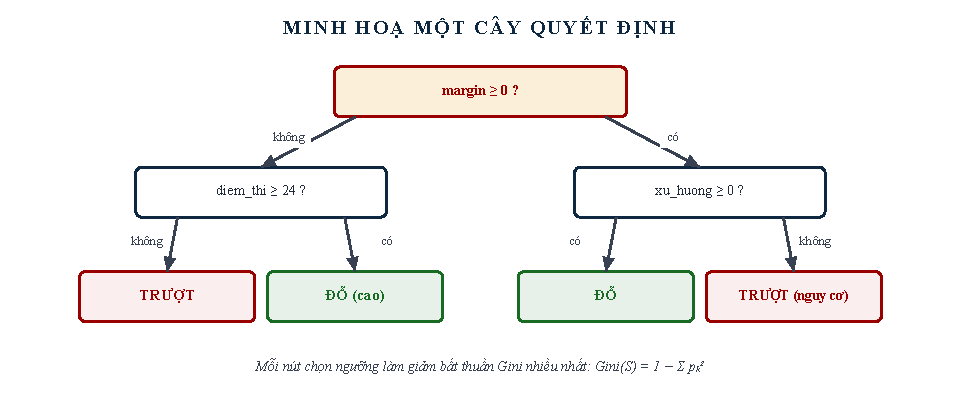
\includegraphics[width=0.92\textwidth]{figs/svg/h-decision-tree.pdf}
\caption{Cây quyết định minh họa với ba tầng phân nhánh theo \code{margin},
\code{diem_thi} và \code{xu_huong}.}
\label{fig:decision-tree}
\end{figure}

Trong Hình~\ref{fig:decision-tree}, nhánh trái của nút gốc ứng với thí sinh có
điểm thấp hơn điểm chuẩn mới nhất (\code{margin} $< 0$). Với nhánh này, mô hình
còn xét thêm \code{diem_thi}: nếu điểm tuyệt đối vẫn cao thì vẫn có khả năng
đỗ do ngành có phổ điểm rộng, ngược lại gần như chắc chắn trượt. Nhánh phải
(\code{margin} $\ge 0$) xét thêm xu hướng biến động: nếu điểm chuẩn đang tăng
nhanh thì mức dư điểm hiện tại chưa đủ an toàn. Ba tầng này chỉ là ví dụ rút
gọn; mô hình thực tế trong đồ án có độ sâu tối đa 14 và học được hàng nghìn
luật tương tự.

\subsection{Ưu điểm và hạn chế}

Cây quyết định có ba ưu điểm đáng chú ý: huấn luyện nhanh, dễ diễn giải và trực
quan hóa logic ra quyết định. Tuy nhiên, một cây đơn lẻ rất dễ quá khớp
\en{(overfitting)} khi mọc quá sâu: cây học thuộc cả nhiễu trong dữ liệu huấn
luyện, dẫn đến phương sai cao và hiệu năng kém trên dữ liệu mới. Đây chính là
động lực cho kỹ thuật tập hợp được trình bày ở mục tiếp theo.

\section{Random Forest}

\subsection{Nguyên lý tập hợp}

Random Forest~\cite{Breiman2001} là kỹ thuật học tập hợp \en{(ensemble
learning)} theo phương pháp đóng bao \en{(bagging)}~\cite{Breiman1996}, kết hợp
thêm ý tưởng chọn ngẫu nhiên không gian con đặc trưng
\en{(random subspace)}~\cite{Ho1995}. Ý tưởng cốt lõi là thay vì tin vào một
cây, ta xây dựng nhiều cây độc lập rồi tổng hợp lại, nhờ đó giảm phương sai mà
gần như không tăng độ chệch.

Mô hình tạo ra $T$ cây theo hai nguồn ngẫu nhiên:

\begin{enumerate}[leftmargin=1.6em, itemsep=3pt]
  \item \textbf{Lấy mẫu bootstrap:} mỗi cây được huấn luyện trên một tập mẫu
        con lấy ngẫu nhiên có hoàn lại từ tập huấn luyện, kích thước bằng tập
        gốc.
  \item \textbf{Chọn ngẫu nhiên đặc trưng:} tại mỗi lần chia nút, cây chỉ xét
        một tập con ngẫu nhiên gồm $m$ đặc trưng. Với bài toán phân loại,
        giá trị mặc định là $m = \lfloor\sqrt{p}\rfloor$; với $p = 27$ đặc
        trưng của đồ án, $m \approx 5$.
\end{enumerate}

Hai nguồn ngẫu nhiên này làm giảm tương quan giữa các cây. Khi các cây ít tương
quan, sai số trung bình của cả rừng nhỏ hơn nhiều so với sai số của từng cây
riêng lẻ.

Kết quả dự đoán xác suất cuối cùng là trung bình xác suất của tất cả các cây:
\begin{equation}
P(y=1 \mid \mathbf{x}) = \frac{1}{T} \sum_{t=1}^{T} P_t(y=1 \mid \mathbf{x}),
\label{eq:rf}
\end{equation}
trong đó $T$ là số cây trong rừng và $P_t$ là xác suất dự đoán của cây thứ $t$.

Hình~\ref{fig:rf} tóm tắt toàn bộ nguyên lý này, từ tập huấn luyện đến kết quả
phân tầng mà người dùng nhìn thấy.

\begin{figure}[H]
\centering
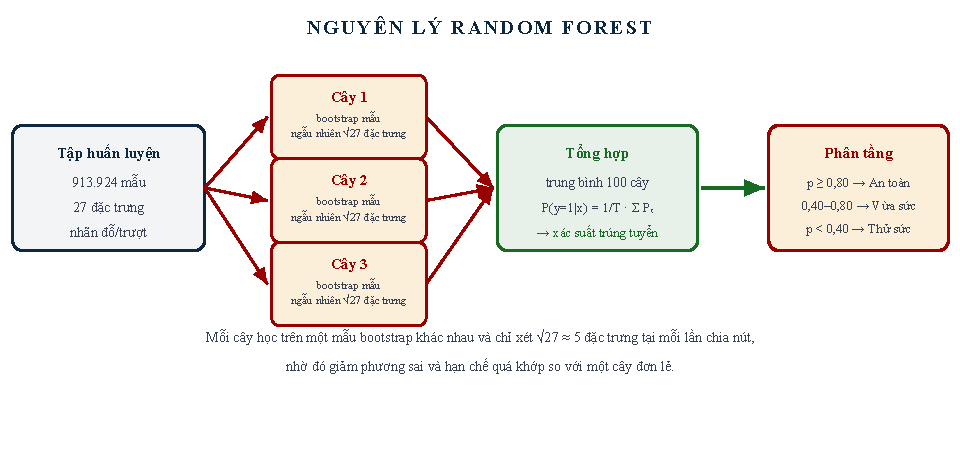
\includegraphics[width=0.95\textwidth]{figs/svg/h-rf.pdf}
\caption{Nguyên lý Random Forest: nhiều cây học trên mẫu bootstrap khác nhau,
tổng hợp bằng trung bình xác suất, rồi phân tầng theo ngưỡng cố định.}
\label{fig:rf}
\end{figure}

\subsection{Vì sao phù hợp với bài toán}

Ba lý do khiến Random Forest là lựa chọn phù hợp:

\begin{itemize}[leftmargin=1.6em, itemsep=3pt]
  \item \textbf{Dữ liệu dạng bảng:} mô hình cây vốn mạnh nhất trên dữ liệu bảng
        có đặc trưng hỗn hợp số và phân loại, đúng với bộ 27 đặc trưng của đồ
        án~\cite{Geron2019}.
  \item \textbf{Không cần chuẩn hóa khắt khe:} cây chỉ so sánh ngưỡng nên ít
        nhạy với thang đo. Tuy vậy đồ án vẫn dùng \code{StandardScaler} để
        thống nhất quy trình và hỗ trợ các mô hình đối chứng.
  \item \textbf{Có sẵn khả năng giải thích:} thuộc tính
        \code{feature_importances_} cho biết mức đóng góp của từng đặc trưng,
        là cơ sở để sinh lời giải thích gợi ý cho người dùng.
\end{itemize}

\subsection{Siêu tham số và ảnh hưởng}

Bảng~\ref{tab:sieu-tham-so} liệt kê các siêu tham số của mô hình chính và lý do
chọn giá trị.

\begin{table}[H]
\centering
\caption{Siêu tham số của Random Forest và căn cứ lựa chọn.}
\label{tab:sieu-tham-so}
\small
\begin{tabularx}{\textwidth}{@{}>{\bfseries\color{daunavy}\raggedright\arraybackslash}m{3.35cm}
  >{\centering\arraybackslash}m{1.85cm}
  >{\raggedright\arraybackslash}X@{}}
\toprule
\rowcolor{gray100}\bfseries\color{daunavy}Siêu tham số & \bfseries\color{daumaroon}Giá trị & \bfseries\color{daunavy}Căn cứ lựa chọn \\
\midrule
\code{n_estimators}      & 100 & Đủ để phương sai hội tụ; tăng lên 200 chỉ cải thiện dưới 0,3\% nhưng file mô hình tăng gấp đôi \\
\code{max_depth}         & 14  & Giới hạn độ sâu để kiểm soát kích thước tệp \code{.pkl} dưới 100~MB \\
\code{min_samples_leaf}  & 5   & Chặn cây tạo lá quá nhỏ, giảm quá khớp trên vùng \code{margin} thưa dữ liệu \\
\code{max_features}      & $\sqrt{27} \approx 5$ & Mặc định của scikit-learn cho phân loại \\
\code{random_state}      & 42  & Bảo đảm kết quả tái lập được giữa các lần chạy \\
\code{n_jobs}            & $-1$ & Dùng toàn bộ nhân CPU khi huấn luyện \\
\bottomrule
\end{tabularx}
\end{table}

Việc chọn giá trị cho từng siêu tham số nêu trên không dựa vào tìm kiếm lưới
\en{(grid search)} toàn diện mà dựa trên ràng buộc kích thước mô hình. Các
nghiên cứu về tối ưu siêu tham số cho thấy tìm kiếm ngẫu nhiên hiệu quả hơn
tìm kiếm lưới khi số chiều lớn~\cite{Bergstra2012}, nhưng với bài toán này chi
phí huấn luyện mỗi cấu hình (hơn 900 nghìn mẫu, 100 cây) khiến việc quét rộng
không khả thi trong phạm vi một học phần. Thay vào đó, hai tham số quyết định
kích thước tệp là \code{n_estimators} và \code{max_depth} được chốt trước theo
ngân sách bộ nhớ, các tham số còn lại giữ mặc định của
scikit-learn~\cite{Pedregosa2011}.

\begin{table}[H]
\centering
\caption{Ảnh hưởng của hai siêu tham số chính lên kích thước mô hình và chất lượng dự đoán.}
\label{tab:quét-tham-so}
\small
\begin{tabularx}{\textwidth}{@{}>{\centering\arraybackslash}m{2.20cm}
  >{\centering\arraybackslash}m{1.75cm}
  >{\centering\arraybackslash}m{2.05cm}
  >{\raggedright\arraybackslash}X
  >{\centering\arraybackslash}m{1.40cm}@{}}
\toprule
\rowcolor{gray100}\bfseries\color{daunavy}\footnotesize\code{n_estimators} &
\bfseries\color{daunavy}\footnotesize\code{max_depth} &
\bfseries\color{daumaroon}Kích thước tệp &
\bfseries\color{daunavy}Ghi chú &
\bfseries\color{daunavy}Quyết định \\
\midrule
50  & 14 & $\approx$ 27~MB  & Phương sai chưa hội tụ hết & Loại \\
100 & 14 & $\approx$ 52~MB  & Cân bằng giữa độ chính xác và bộ nhớ & \textbf{Chọn} \\
200 & 14 & $\approx$ 104~MB & Vượt ngân sách 100~MB; cải thiện dưới 0,3\% & Loại \\
100 & 20 & $\approx$ 96~MB  & Sát ngưỡng, dễ quá khớp vùng \code{margin} thưa & Loại \\
\bottomrule
\end{tabularx}
\end{table}

Bảng~\ref{tab:quét-tham-so} giải thích vì sao cấu hình 100 cây và độ sâu 14
được chọn thay vì những cấu hình ``mạnh'' hơn. Cột kích thước là yếu tố quyết
định: mô hình phải nạp trọn vào RAM của máy chủ 2~GB, nên ngưỡng 100~MB là
ràng buộc cứng chứ không phải mục tiêu tối ưu. Hai cấu hình bị loại ở hai phía
khác nhau: 50 cây chưa đủ để phương sai hội tụ, còn 200 cây vượt ngân sách bộ
nhớ mà chỉ cải thiện dưới 0,3\%. Cấu hình độ sâu 20 bị loại vì vừa sát ngưỡng
dung lượng vừa có nguy cơ quá khớp ở vùng \code{margin} thưa dữ liệu --- đúng
vùng mà hệ thống cần dự đoán chính xác nhất.

Bảng~\ref{tab:sieu-tham-so} cho thấy mọi siêu tham số đều được chốt vì một
ràng buộc kỹ thuật cụ thể chứ không phải chọn tùy ý. Ràng buộc chi phối toàn bộ
quá trình là kích thước tệp mô hình: hệ thống phải nạp \code{model.pkl} vào RAM
của một máy chủ phổ thông, nên độ sâu và số cây bị giới hạn có chủ đích. Đánh
đổi này được đánh giá định lượng ở Chương~\ref{ch:caidat}.

\section{Các chỉ số đánh giá mô hình}

Để đánh giá toàn diện khả năng dự báo xác suất trúng tuyển, đồ án sử dụng bốn
nhóm chỉ số trên tập kiểm thử độc lập năm 2025. Bảng~\ref{tab:chi-so} tóm tắt
công thức và ý nghĩa từng chỉ số.

\begin{table}[H]
\centering
\caption{Các chỉ số đánh giá mô hình và ý nghĩa trong bối cảnh bài toán.}
\label{tab:chi-so}
\begin{tabularx}{\textwidth}{>{\bfseries\color{daunavy}}l >{\raggedright\arraybackslash}p{4.4cm} >{\raggedright\arraybackslash}X}
\toprule
\rowcolor{gray100}\bfseries\color{daunavy}Chỉ số & \bfseries\color{daunavy}Công thức & \bfseries\color{daunavy}Ý nghĩa với hệ thống \\
\midrule
Accuracy & $\dfrac{TP + TN}{TP + TN + FP + FN}$ & Hiệu năng tổng thể; dễ gây hiểu lầm nếu hai lớp mất cân bằng \\
Precision & $\dfrac{TP}{TP + FP}$ & Khi hệ thống nói ``khả năng đỗ cao'', điều đó có đáng tin không \\
Recall & $\dfrac{TP}{TP + FN}$ & Hệ thống có bỏ sót cơ hội đỗ thực sự của thí sinh không \\
ROC-AUC & Diện tích dưới đường cong ROC & Khả năng xếp hạng Đỗ/Trượt trên mọi ngưỡng~\cite{Fawcett2006} \\
Brier & $\dfrac{1}{N}\sum_{i=1}^{N}(p_i - y_i)^2$ & Mức hiệu chuẩn của xác suất~\cite{Brier1950} \\
F1 & $2\cdot\dfrac{Precision \cdot Recall}{Precision + Recall}$ & Trung bình điều hòa, cân bằng giữa bỏ sót và báo nhầm \\
\bottomrule
\end{tabularx}
\end{table}

Chỉ số Brier đóng vai trò đặc biệt quan trọng trong đồ án này. Hệ thống không
chỉ dùng mô hình để phân loại nhị phân đỗ/trượt mà còn dùng trực tiếp giá trị
xác suất $p$ để chia ba tầng. Nếu mô hình dự đoán $p = 0{,}9$ nhưng tỷ lệ đỗ
thực tế chỉ là $0{,}6$, thì phân tầng ``An toàn'' sẽ sai và người dùng bị đánh
lừa về mức độ an toàn. Brier score đo chính xác loại sai lệch này, nên nó là
chỉ số then chốt dù ít quen thuộc hơn Accuracy.

\section{Công nghệ và thư viện}

Hệ thống Uni Connect được xây dựng hoàn toàn trên ngôn ngữ Python và các công
nghệ mã nguồn mở phổ biến. Bảng~\ref{tab:congcu} liệt kê chi tiết.

\begin{table}[H]
\centering
\caption{Công cụ và thư viện sử dụng trong đồ án Uni Connect.}
\label{tab:congcu}
\begin{tabularx}{\textwidth}{>{\bfseries\color{daunavy}}l >{\color{daumaroon}}l >{\raggedright\arraybackslash}X}
\toprule
\rowcolor{gray100}\bfseries\color{daunavy}Thành phần & \bfseries\color{daumaroon}Phiên bản & \bfseries\color{daunavy}Vai trò \\
\midrule
Python         & 3.13              & Ngôn ngữ lập trình chính của toàn hệ thống~\cite{VanderPlas2016} \\
Django         & 5.2.8             & Framework web: định tuyến, ORM, xác thực, quản trị~\cite{DjangoDocs} \\
MySQL          & 8.0               & Hệ quản trị cơ sở dữ liệu quan hệ chính~\cite{MySQLDocs} \\
scikit-learn   & 1.8.0             & Huấn luyện mô hình Random Forest~\cite{Pedregosa2011} \\
pandas         & 3.0.2             & Đọc, xử lý và chuẩn hóa dữ liệu dạng bảng~\cite{McKinney2017} \\
NumPy          & 2.3.3             & Tính toán vector, trích xuất đặc trưng chuỗi thời gian \\
joblib         & đi kèm sklearn    & Lưu trữ và nạp mô hình, bộ chuẩn hóa \\
Tailwind CSS   & qua CDN           & Thiết kế giao diện người dùng đáp ứng \\
\bottomrule
\end{tabularx}
\end{table}

Bảng~\ref{tab:congcu} cho thấy toàn bộ hệ thống nằm trong một ngăn xếp công
nghệ đồng nhất về ngôn ngữ Python, giúp giảm chi phí chuyển đổi ngữ cảnh giữa
phân hệ huấn luyện và phân hệ phục vụ. Django được chọn vì có sẵn ORM, hệ thống
xác thực và trang quản trị; MySQL được chọn vì phổ biến trên các gói hosting
sinh viên. Việc dùng \code{managed = False} cho các model Django (trình bày ở
Chương~\ref{ch:thietke}) là một quyết định kiến trúc quan trọng: lược đồ do tệp
SQL quản lý, còn Django chỉ đọc.

\section{Quy trình phát triển phần mềm}

Đồ án theo mô hình thác nước cải tiến \en{(iterative waterfall)} phù hợp với
phạm vi một học phần: yêu cầu được chốt sớm, nhưng mỗi vòng lặp có kiểm thử và
điều chỉnh~\cite{Somerville2015}. Bốn giai đoạn chính:

\begin{enumerate}[leftmargin=1.6em, itemsep=3pt]
  \item \textbf{Phân tích yêu cầu:} xác định tác nhân, ca sử dụng và yêu cầu
        phi chức năng (Chương~\ref{ch:thietke}).
  \item \textbf{Thiết kế:} kiến trúc bốn tầng, lược đồ cơ sở dữ liệu và bộ đặc
        trưng (Chương~\ref{ch:thietke}).
  \item \textbf{Cài đặt và thử nghiệm:} viết mã nguồn, kiểm thử ba cấp độ
        (Chương~\ref{ch:caidat}).
  \item \textbf{Đánh giá:} đo mô hình trên tập kiểm thử độc lập, đối chiếu mục
        tiêu (cùng Chương~\ref{ch:caidat}).
\end{enumerate}

\section{Các công trình liên quan}

Bài toán gợi ý nguyện vọng cho thí sinh xét tuyển đã được nhiều đơn vị trong
nước tiếp cận theo hai hướng chính.

\textbf{Hướng thứ nhất} là các cổng tra cứu thông tin tuyển sinh trực tuyến
như cổng thông tin của Bộ Giáo dục và Đào tạo hay các trang báo điện tử tổng
hợp điểm chuẩn. Ưu điểm của hướng này là dữ liệu phong phú, nhưng nhược điểm
là chỉ hiển thị bảng điểm thô: người dùng vẫn phải tự so sánh và tự phán đoán
rủi ro.

\textbf{Hướng thứ hai} là các ứng dụng tư vấn sử dụng trí tuệ nhân tạo. Một số
nghiên cứu tiêu biểu sử dụng thuật toán Random Forest trên dữ liệu giáo dục đã
chứng minh hiệu quả vượt trội của mô hình tập hợp so với mô hình tuyến tính
đơn lẻ~\cite{Breiman2001,Hastie2009}. Các giáo trình nền tảng về trí tuệ nhân
tạo cũng đặt cơ sở lý thuyết vững chắc cho các kỹ thuật học có giám sát và
đánh giá mô hình~\cite{HoangKiem,RussellNorvig2021}.

\textbf{Đóng góp riêng của đồ án} nằm ở ba điểm. Thứ nhất là độ sâu dữ liệu:
chuỗi lịch sử 10 năm liên tục (2016--2025) thay vì 1--2 năm gần nhất, giúp mô
hình nắm bắt xu hướng dài hạn. Thứ hai là tính minh bạch: hệ thống không chỉ
trả con số xác suất mà sinh kèm lời giải thích dựa trên các chỉ số thống kê cụ
thể mà phụ huynh đọc hiểu được. Thứ ba là tính trọn vòng đời: hệ thống vận hành
khép kín từ thu thập dữ liệu, huấn luyện mô hình đến phục vụ người dùng, kèm cơ
chế cửa sổ trượt để cập nhật dữ liệu hằng năm mà không cần sửa mã nguồn.

\section{Tổng kết chương}

Chương này đã thiết lập bốn nền tảng: bài toán phân loại nhị phân với đặc thù
phi tuyến, cây quyết định và cơ chế tập hợp của Random Forest, bộ chỉ số đánh
giá (đặc biệt là Brier score cho bài toán dùng trực tiếp xác suất), và ngăn xếp
công nghệ Python--Django--MySQL. Chương~\ref{ch:thietke} sẽ áp dụng các nền
tảng này để thiết kế kiến trúc, cơ sở dữ liệu và bộ đặc trưng cụ thể.

\chapter{Phân tích và thiết kế}
\label{ch:thietke}

\section{Phân tích bài toán và yêu cầu}

\subsection{Đầu vào và đầu ra của hệ thống}

\textbf{Đầu vào} của hệ thống gợi ý trung tâm bao gồm hồ sơ năng lực do học sinh nhập:
\begin{itemize}[leftmargin=1.6em, itemsep=2pt]
  \item Điểm thi từng môn học (thang 10) và điểm học bạ trung bình các môn.
  \item Tổ hợp môn xét tuyển mà học sinh có thể sử dụng (ví dụ: A00 --- Toán, Lý, Hóa).
  \item Nhóm ngành đào tạo ưu tiên và khu vực địa lý mong muốn trong số 15 nhóm ngành và 3 vùng miền.
\end{itemize}

\textbf{Đầu ra} là danh sách tối đa 30 nguyện vọng (mỗi nguyện vọng là một bộ: trường, ngành, tổ hợp, phương thức) được sắp xếp theo xác suất trúng tuyển giảm dần và phân thành 3 tầng trực quan: Tầng \textbf{An toàn} ($p \ge 0{,}80$) dùng làm phương án dự phòng chắc chắn; tầng \textbf{Vừa sức} ($0{,}40 \le p < 0{,}80$) là nhóm lựa chọn chính phù hợp năng lực; tầng \textbf{Thử sức} ($p < 0{,}40$) là nhóm kỳ vọng cao dành cho ngành yêu thích.

\subsection{Yêu cầu chức năng}

Hệ thống bao gồm 11 ca sử dụng \en{(Use Case)} chính, chia theo ba nhóm tác nhân: Khách (tra cứu, xem chi tiết trường), Học sinh đã đăng nhập (nhập hồ sơ điểm, nhận gợi ý AI, xem lời giải thích, so sánh và lưu nguyện vọng) và Quản trị viên (cập nhật dữ liệu năm mới, huấn luyện lại mô hình, xem thống kê). Hai ca sử dụng trung tâm có AI tham gia là UC-05 (Nhận gợi ý trường, ngành) và UC-10 (Huấn luyện lại mô hình). Toàn cảnh quan hệ giữa các tác nhân và các ca sử dụng được thể hiện ở Hình~\ref{fig:usecase}.

\begin{figure}[H]
\centering
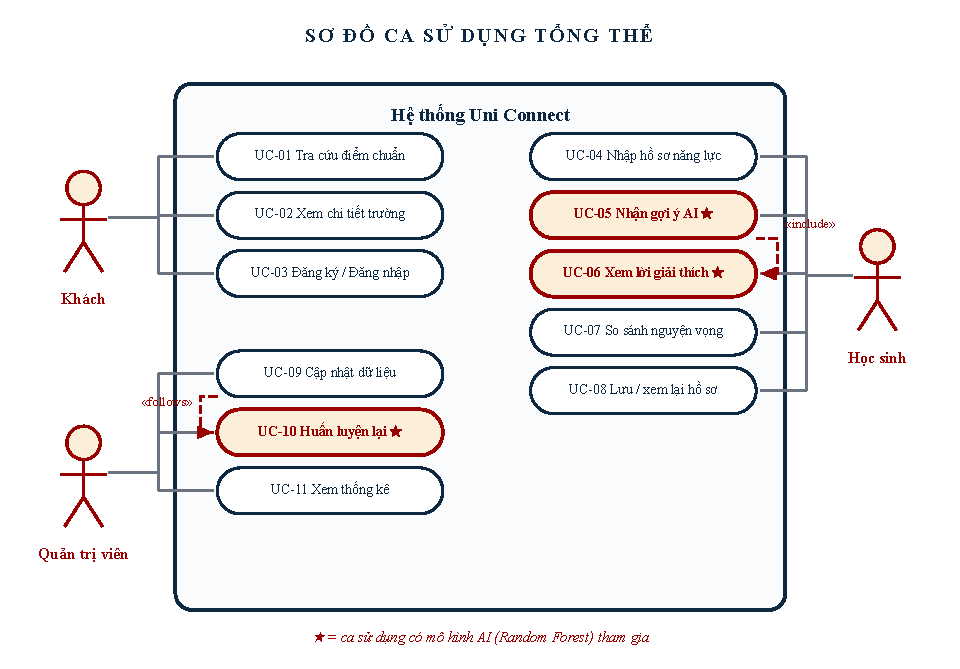
\includegraphics[width=\textwidth]{figs/svg/h-usecase.pdf}
\caption{Sơ đồ ca sử dụng (Use Case) tổng thể của hệ thống Uni Connect.}
\label{fig:usecase}
\end{figure}

Mười một ca sử dụng trên được phân rã thành năm nhóm chức năng theo mô hình cây như Hình~\ref{fig:bfd}. Cách phân rã này bám sát cấu trúc thư mục mã nguồn thật của đồ án: mỗi nhóm chức năng tương ứng một ứng dụng Django độc lập.

\begin{figure}[H]
\centering
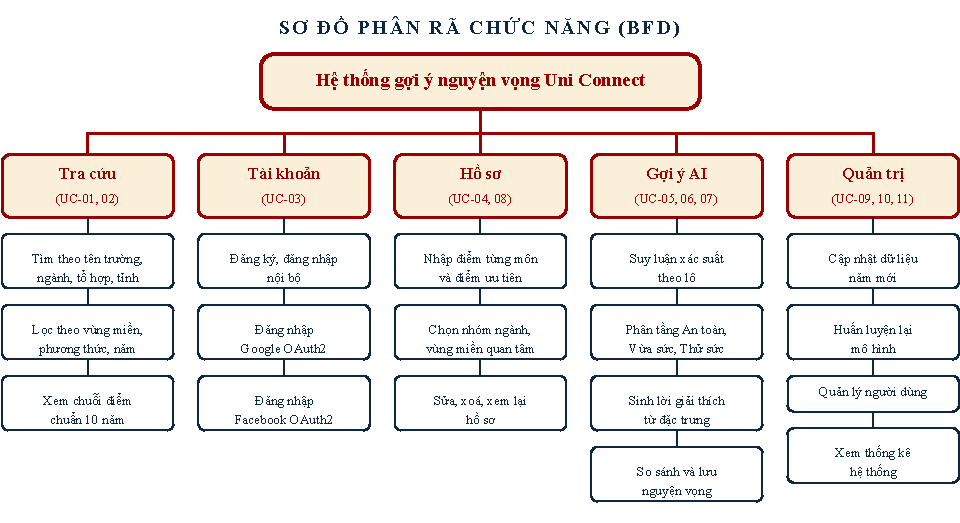
\includegraphics[width=\textwidth]{figs/svg/h-bfd.pdf}
\caption{Sơ đồ phân rã chức năng (BFD) của hệ thống Uni Connect.}
\label{fig:bfd}
\end{figure}

\textbf{Tiêu chí hệ thống chạy đúng:}
\begin{itemize}[leftmargin=1.6em, itemsep=2pt]
  \item Mọi điểm chuẩn hiển thị trên giao diện phải trùng khớp tuyệt đối với bản ghi đã lưu trong cơ sở dữ liệu.
  \item Với cùng một hồ sơ đầu vào, danh sách gợi ý sinh ra phải nhất quán và có thứ tự xếp hạng ổn định.
  \item Ngưỡng phân tầng 0,80 và 0,40 được khai báo công khai rõ ràng trên giao diện, không để người dùng tự ước đoán.
\end{itemize}

\subsection{Yêu cầu phi chức năng}
\label{sec:nfr}

\begin{itemize}[leftmargin=1.6em, itemsep=2pt]
  \item \textbf{Hiệu năng} (PC-01): Trang gợi ý AI phải phản hồi trong vòng dưới 3 giây trên hạ tầng máy chủ thông thường; mô hình \code{model.pkl} (~52~MB) chỉ nạp một lần vào RAM khi khởi động tiến trình, không đọc lại đĩa cứng mỗi lượt truy vấn.
  \item \textbf{Độ tin cậy:} Mọi lỗi liên quan đến mô hình (thiếu file, sai lệch phiên bản thư viện) đều không được gây lỗi hệ thống 500. Hệ thống tự động chuyển sang chế độ dự phòng (xếp hạng bằng \code{margin} thuần) và ghi rõ trạng thái ``chưa dùng mô hình AI''.
  \item \textbf{Khả năng mở rộng:} Cơ chế cửa sổ trượt cho phép cập nhật dữ liệu năm mới (ví dụ: năm 2026) mà không cần thay đổi cấu trúc bảng hay viết lại mã nguồn xử lý.
\end{itemize}

\section{Thiết kế kiến trúc hệ thống}

Kiến trúc tổng thể của hệ thống Uni Connect được trình bày ở Hình~\ref{fig:kientruc}. Dữ liệu vận hành theo luồng khép kín gồm 4 tầng chính.

\begin{figure}[H]
\centering
\resizebox{\textwidth}{!}{%
\begin{tikzpicture}[node distance=10mm and 12mm]
  \node[objbox] (crawl) {Thu thập\\(crawler, CSV)};
  \node[clsbox, right=of crawl] (db) {CSDL MySQL\\(15 bảng quan hệ)};
  \node[clsbox, right=of db] (model) {Mô hình AI\\(Random Forest)};
  \node[clsbox, right=of model] (web) {Django Web\\(tra cứu, gợi ý)};
  \node[objbox, right=of web] (user) {Học sinh,\\quản trị viên};
  \draw[flowarr] (crawl) -- (db);
  \draw[flowarr] (db) -- (model);
  \draw[flowarr] (model) -- (web);
  \draw[flowarr] (web) -- (user);
  \draw[flowarr] (user) |- ($(web.south)+(0,-6mm)$) -| (web);
\end{tikzpicture}}
\caption{Sơ đồ kiến trúc tổng thể của hệ thống gợi ý nguyện vọng Uni Connect.}
\label{fig:kientruc}
\end{figure}

Luồng hoạt động cụ thể như sau: (1) Bộ thu thập ngoại tuyến \code{crawl_diemchuan.py} tự động tải, làm sạch dữ liệu và xuất ra các file CSV chuẩn; (2) Script \code{import_mysql.py} nạp dữ liệu vào CSDL MySQL; (3) Pipeline huấn luyện \code{gen_dataset.py} trích xuất đặc trưng và \code{train.py} sinh ra mô hình \code{model.pkl}; (4) Ứng dụng web Django phục vụ người dùng cuối, gọi mô hình khi có yêu cầu gợi ý thông qua module suy luận \code{predict.py}.

\section{Sơ đồ luồng xử lý nghiệp vụ}

\subsection{UC-03 Đăng ký / Đăng nhập}

Luồng xử lý tài khoản bao gồm khóa tạm theo tỷ lệ sai khi đăng nhập, cơ chế dự phòng cho dịch vụ.

\begin{figure}[H]
\centering
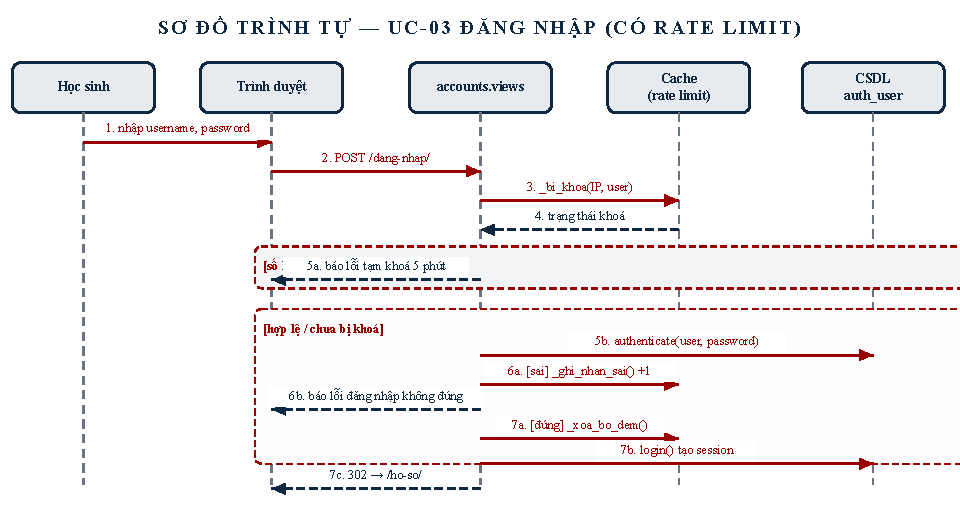
\includegraphics[width=\textwidth]{figs/svg/h-seq-dangnhap.pdf}
\caption{Sơ đồ trình tự UC-03 Đăng nhập (với cơ chế rate limit và câu trả lời dự phòng).}
\label{fig:seq-dangnhap}
\end{figure}

\subsection{UC-05 Nhận gợi ý (AI)}

Luồng xử lý nhận gợi ý dung sự khía cạnh: mô hình AI khi sẵn sàng, cơ chế dự phòng xếp hạng theo margin khi mô hình lỗi.

\begin{figure}[H]
\centering
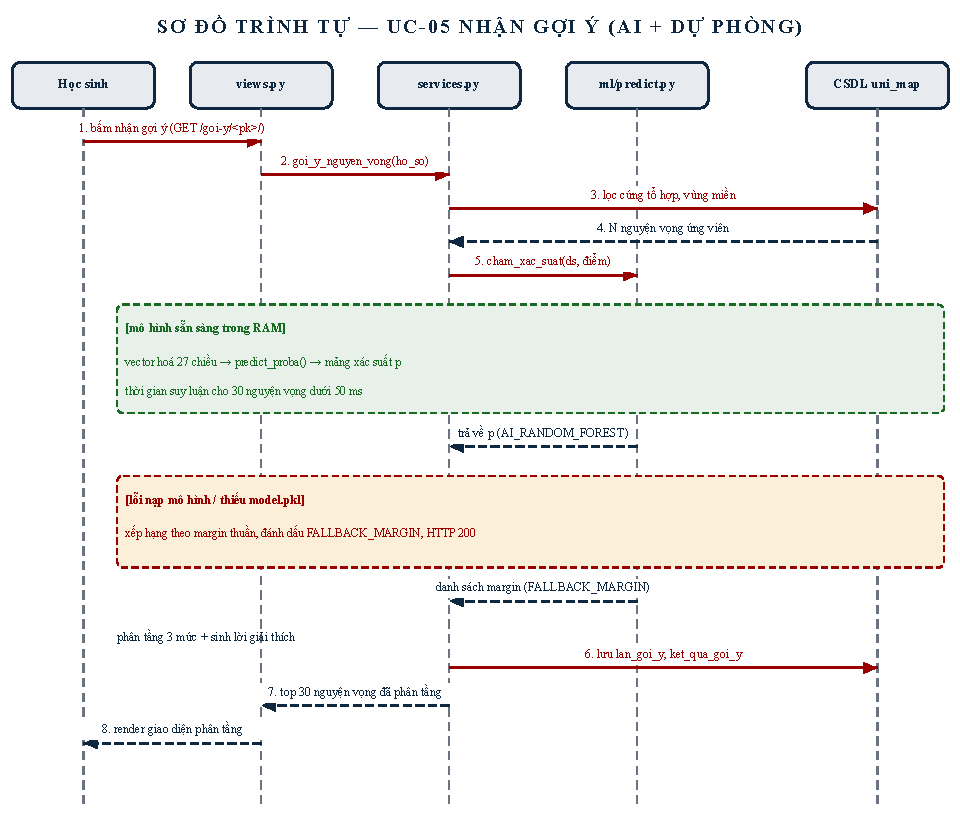
\includegraphics[width=\textwidth]{figs/svg/h-seq-goiy.pdf}
\caption{Sơ đồ trình tự UC-05 Nhận gợi ý (AI dự phòng xếp hạng theo margin khi lỗi mô hình).}
\label{fig:seq-goiy}
\end{figure}

\subsection{UC-09 + UC-10 Cập nhật dữ liệu và huấn luyện lại mô hình}

Luồng cập nhật dữ liệu năm mới và huấn luyện lại mô hình AI.

\begin{figure}[H]
\centering
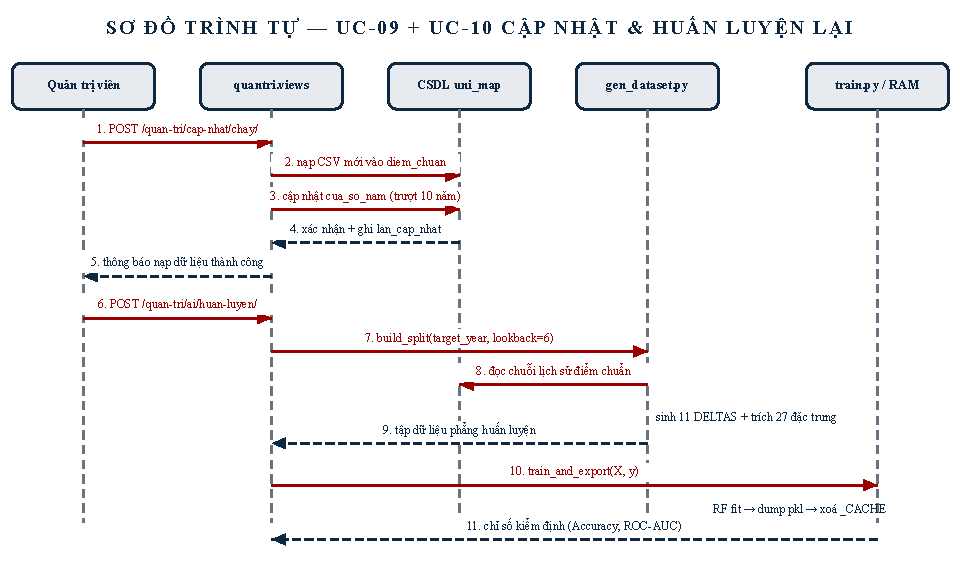
\includegraphics[width=\textwidth]{figs/svg/h-seq-capnhat.pdf}
\caption{Sơ đồ trình tự UC-09 + UC-10 Cập nhật dữ liệu năm mới và huấn luyện lại mô hình AI.}
\label{fig:seq-capnhat}
\end{figure}

Chi tiết định tuyến từ yêu cầu HTTP tới từng tầng xử lý được thể hiện ở Hình~\ref{fig:api}. Toàn bộ endpoint trong sơ đồ đều lấy nguyên văn từ bảy file \code{urls.py} của các ứng dụng Django (\code{university}, \code{api}, \code{accounts}, \code{admissions}, \code{recommendation}, \code{quantri}).

\begin{figure}[H]
\centering
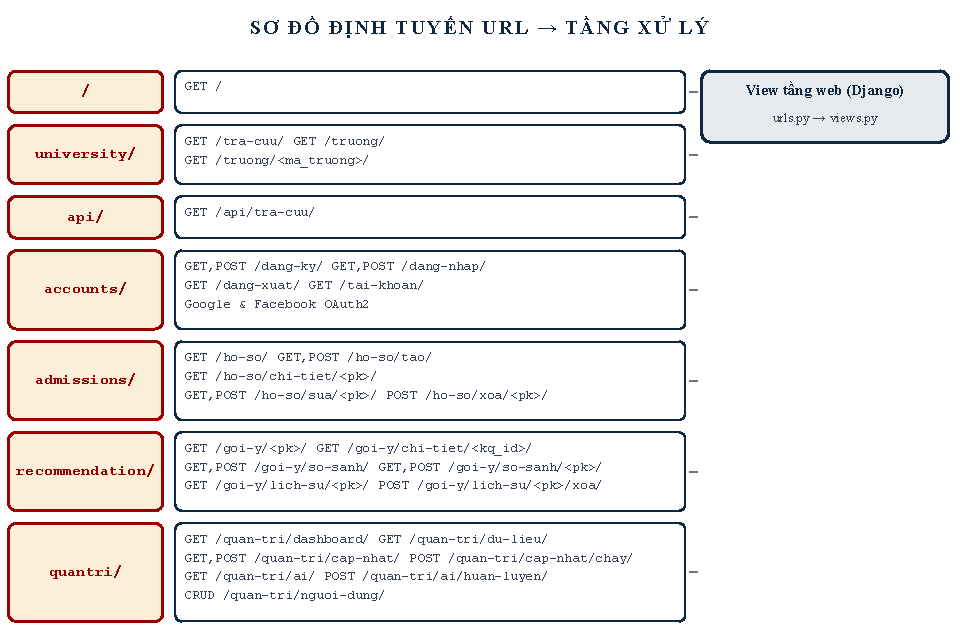
\includegraphics[width=\textwidth]{figs/svg/h-api.pdf}
\caption{Sơ đồ định tuyến API và URL của hệ thống Uni Connect.}
\label{fig:api}
\end{figure}

\section{Thiết kế dữ liệu}

\subsection{Nguồn và quy mô dữ liệu}

Dữ liệu điểm chuẩn được thu thập từ cổng tổng hợp \code{diemthi.tuyensinh247.com}. Quy trình thu thập tự động xử lý các tình huống thực tế phức tạp như lỗi font chữ tiếng Việt của nguồn, cơ chế công bố điểm nhỏ giọt kéo dài suốt mùa tuyển sinh và tự động chặn các năm chưa đủ dữ liệu tin cậy. Tổng quy mô dữ liệu thực tế sau khi chuẩn hóa được thống kê ở Bảng~\ref{tab:dulieu}.

\begin{table}[H]
\centering
\caption{Quy mô cơ sở dữ liệu điểm chuẩn thực tế của hệ thống Uni Connect.}
\label{tab:dulieu}
\begin{tabularx}{\textwidth}{>{\bfseries\color{daunavy}}l >{\color{daumaroon}\bfseries}r >{\raggedright\arraybackslash}X}
\toprule
\rowcolor{gray100}\bfseries\color{daunavy}Hạng mục dữ liệu & \bfseries\color{daumaroon}Số lượng & \bfseries\color{daunavy}Ghi chú \\
\midrule
Trường đại học         & 295        & Mã trường là khóa chính, phủ 3 miền Bắc -- Trung -- Nam \\
Ngành đào tạo          & 3.037      & Gom nhóm thành 15 nhóm ngành chuẩn \\
Tổ hợp xét tuyển       & 340        & Ví dụ: A00, B00, D01, C00 \\
Bản ghi điểm chuẩn     & 240.483    & Fact (trường, ngành, tổ hợp, phương thức, năm) \\
Chuỗi đặc trưng        & 100.363    & Dòng thống kê chuỗi 10 năm cho mỗi nguyện vọng \\
Cửa sổ dữ liệu         & 2016--2025 & 10 năm liên tục, hiển thị đầy đủ; AI dùng 6 năm gần nhất \\
\bottomrule
\end{tabularx}
\end{table}

\subsection{Lược đồ cơ sở dữ liệu}

\begin{figure}[H]
\centering
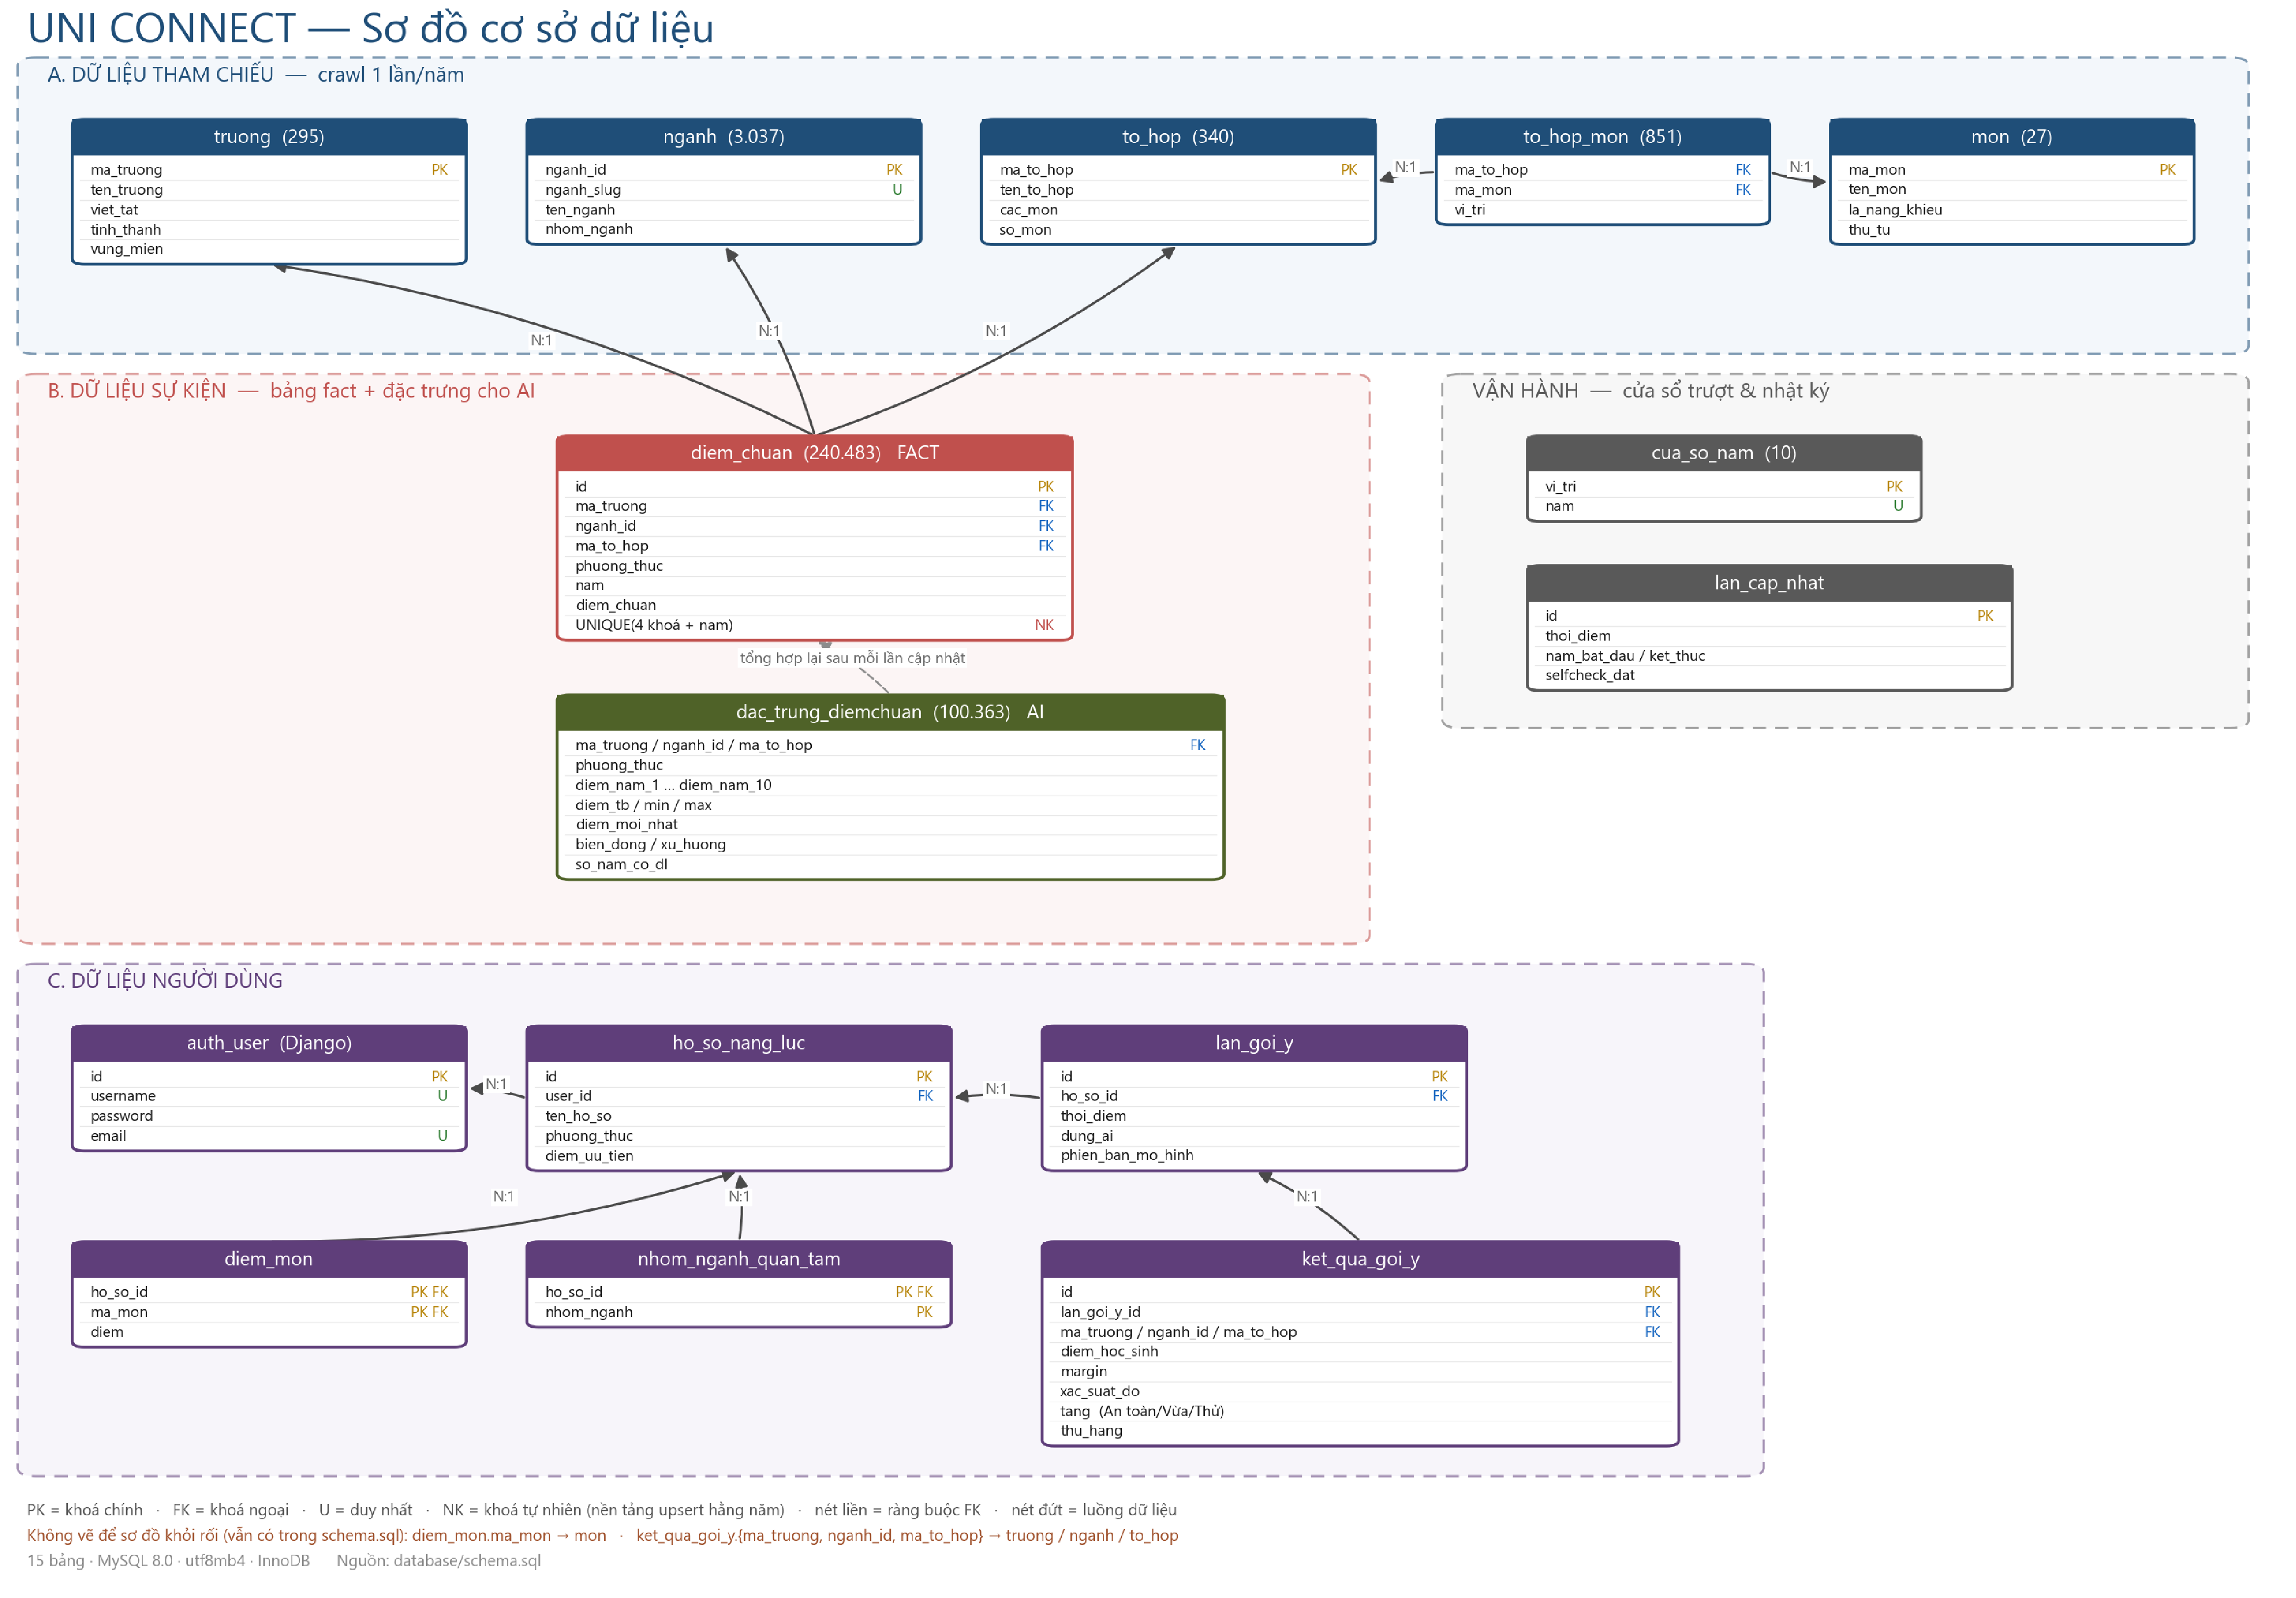
\includegraphics[width=\textwidth]{figs/svg/h-erd-source.pdf}
\caption{Lược đồ quan hệ ERD của cơ sở dữ liệu \code{uni_map}, lấy từ sơ đồ CSDL thực tế của hệ thống.}
\label{fig:erd}
\end{figure}

Cơ sở dữ liệu quan hệ \code{uni_map} bao gồm 15 bảng, quan hệ giữa chúng được
tóm tắt ở Hình~\ref{fig:erd}. Trong đó \code{db/schema.sql} là nguồn chân lý duy
nhất của lược đồ (các model Django đặt \code{managed = False} và không sinh
migration cho các bảng nghiệp vụ) --- cùng nguyên tắc tách lược đồ khỏi mã ứng
dụng được bàn trong~\cite{Fowler2002}.

Hình~\ref{fig:erd} chia 15 bảng thành bốn nhóm chức năng, và cách chia này phản
ánh trực tiếp vòng đời dữ liệu của hệ thống. Nhóm \en{tham chiếu} gồm
\code{truong}, \code{nganh}, \code{mon}, \code{to_hop} và \code{to_hop_mon} quản
lý danh mục và chỉ thay đổi khi có trường hoặc ngành mới. Nhóm \en{sự kiện} gồm
\code{diem_chuan} --- bảng fact trung tâm lưu điểm trúng tuyển của từng bộ
(trường, ngành, tổ hợp, phương thức, năm) --- và \code{dac_trung_diemchuan} lưu
10 cột điểm thô \code{diem_nam_1} đến \code{diem_nam_10} cùng các chỉ số thống
kê đã tính sẵn (\code{diem_tb}, \code{diem_min}, \code{diem_max},
\code{diem_moi_nhat}, \code{bien_dong}, \code{xu_huong}, \code{so_nam_co_dl}).
Nhóm \en{vận hành} gồm \code{cua_so_nam} và \code{lan_cap_nhat} phục vụ cơ chế
trượt cửa sổ và ghi vết mỗi lần nạp dữ liệu. Nhóm \en{người dùng} gồm
\code{auth\_user} của Django cùng bốn bảng hồ sơ và kết quả gợi ý
(\code{ho_so_nang_luc}, \code{diem_mon}, \code{nhom_nganh_quan_tam},
\code{lan_goi_y}, \code{ket_qua_goi_y}).

Điểm thiết kế nổi bật là bảng \code{cua_so_nam} ánh xạ vị trí cột ($1$--$10$) sang năm thực tế (2016--2025). Khi cập nhật dữ liệu năm 2026, quản trị viên chỉ cần thay đổi ánh xạ này qua giao diện mà hệ thống tự trượt cửa sổ hiển thị, không cần thực hiện lệnh \code{ALTER TABLE} hay sửa đổi mã nguồn (yêu cầu CN-05).

\section{Thiết kế mô hình và bộ đặc trưng}

\subsection{Chiến lược sinh nhãn huấn luyện}

Do không tồn tại dữ liệu đỗ/trượt thực tế của thí sinh trong quá khứ (giả định GĐ-3), đồ án áp dụng kỹ thuật sinh mẫu giả lập từ lịch sử: mỗi bản ghi điểm chuẩn $C$ của năm mục tiêu $t$ được xem là một ``sự thật tuyển sinh'' --- thí sinh giả lập có điểm thi $X$ xung quanh $C$ sẽ đỗ nếu $X \ge C$. Cụ thể, với mỗi nguyện vọng, 11 mức chênh lệch \code{DELTAS} $= \{-3{,}0; -2{,}0; -1{,}0; -0{,}5; -0{,}2; 0{,}0; +0{,}2; +0{,}5; +1{,}0; +2{,}0; +3{,}0\}$ được cộng vào điểm chuẩn gốc để tạo ra 11 mẫu huấn luyện có nhãn cân bằng.

Để ngăn chặn tuyệt đối hiện tượng rò rỉ dữ liệu \en{(data leakage)} --- hiện
tượng đã được phân loại và mô tả có hệ thống trong~\cite{Kaufman2012} --- đặc
trưng của mẫu năm mục tiêu $t$ chỉ được phép tính toán từ các năm quá khứ nhỏ
hơn $t$. Đồng thời, tập dữ liệu được chia cứng theo mốc thời gian: huấn luyện
trên các năm 2021--2024 và kiểm thử hoàn toàn độc lập trên năm 2025. Cách chia
này khác với kiểm định chéo $k$-fold thông thường: nếu trộn ngẫu nhiên các mẫu
của mọi năm rồi chia $k$ phần, mẫu của năm 2025 sẽ xuất hiện trong cả tập huấn
luyện lẫn tập kiểm thử và kết quả đo trở nên vô nghĩa.

\subsection{Bộ 27 đặc trưng và siêu tham số}

Vector đầu vào của mô hình gồm 27 chiều, thứ tự được cố định nghiêm ngặt trong file \code{constants.py} để đảm bảo tính nhất quán giữa giai đoạn huấn luyện và suy luận: 7 đặc trưng số (\code{diem_thi}, \code{margin}, \code{diem_moi_nhat}, \code{diem_tb}, \code{xu_huong}, \code{bien_dong}, \code{so_nam_co_dl}), 15 cột mã hóa \en{one-hot} nhóm ngành, 3 cột vùng miền và 2 cột phương thức xét tuyển. Bảng~\ref{tab:dactrung} liệt kê đầy đủ 27 đặc trưng theo bốn nhóm cùng vai trò của từng nhóm trong bài toán dự đoán.

\begin{table}[H]
\centering
\caption{Bộ 27 đặc trưng đầu vào của mô hình, chia thành bốn nhóm theo bản chất thông tin.}
\label{tab:dactrung}
\small
\begin{tabularx}{\textwidth}{@{}>{\raggedright\arraybackslash\strut}p{2.45cm}
  >{\centering\arraybackslash\strut}p{1.05cm}
  >{\raggedright\arraybackslash\strut}X
  >{\raggedright\arraybackslash\strut}p{3.15cm}@{}}
\toprule
\rowcolor{gray100}\bfseries\color{daunavy}Nhóm đặc trưng &
\bfseries\color{daumaroon}Số chiều &
\bfseries\color{daunavy}Thành phần (tên cột trong \code{constants.py}) &
\bfseries\color{daunavy}Vai trò trong dự đoán \\
\midrule
Đặc trưng số & 7 &
\code{diem_thi}, \code{margin}, \code{diem_moi_nhat}, \code{diem_tb},
\code{xu_huong}, \code{bien_dong}, \code{so_nam_co_dl} &
Mô tả trực tiếp năng lực thí sinh và diễn biến lịch sử của ngành \\
\addlinespace[2pt]
Nhóm ngành & 15 &
Mã hóa \en{one-hot} cho 15 nhóm ngành chuẩn, tiền tố \code{nn_}:
Báo chí -- Truyền thông; Công nghệ thông tin; Du lịch -- Khách sạn -- Nhà hàng;
Khác; Khoa học XH \& Nhân văn; Kiến trúc -- Xây dựng; Kinh tế -- Kinh doanh -- Tài chính;
Kỹ thuật -- Công nghệ; Luật; Nghệ thuật -- Thiết kế -- TDTT; Ngôn ngữ -- Quốc tế học;
Nông -- Lâm -- Ngư -- Thú y; Quân đội -- Công an; Sư phạm -- Giáo dục; Y -- Dược -- Sức khỏe &
Phản ánh mức cạnh tranh đặc thù của từng lĩnh vực đào tạo \\
\addlinespace[2pt]
Vùng miền & 3 &
\code{vm_Miền Bắc}, \code{vm_Miền Trung}, \code{vm_Miền Nam} &
Hiệu chỉnh khác biệt mặt bằng điểm theo khu vực địa lý \\
\addlinespace[2pt]
Phương thức & 2 &
\code{pt_Điểm thi THPT}, \code{pt_Điểm học bạ} &
Phân biệt khác biệt về thang điểm và phân bố giữa hai phương thức \\
\midrule
\rowcolor{gray100}\bfseries Tổng cộng & \bfseries\color{daumaroon}27 &
\bfseries 7 số + 15 nhóm ngành + 3 vùng miền + 2 phương thức &
\bfseries Thứ tự cố định, khớp tuyệt đối giữa huấn luyện và suy luận \\
\bottomrule
\end{tabularx}
\end{table}

Bảng~\ref{tab:dactrung} cho thấy bốn nhóm đặc trưng không ngang hàng về số chiều nhưng bổ sung cho nhau theo ba lớp thông tin. Lớp thứ nhất là năng lực cá nhân, gồm \code{diem_thi} và \code{margin} --- hai biến quyết định phần lớn kết quả dự đoán. Lớp thứ hai là bối cảnh lịch sử của ngành, gồm bốn chỉ số thống kê chuỗi thời gian còn lại. Lớp thứ ba là bối cảnh phân loại, gồm 20 cột \en{one-hot} cho nhóm ngành, vùng miền và phương thức xét tuyển. Việc tách 15 nhóm ngành thành 15 cột nhị phân thay vì một cột số nguyên là lựa chọn có chủ đích: cây quyết định chỉ so sánh được ngưỡng số, nên nếu mã hóa nhóm ngành thành các số 1--15 thì mô hình sẽ ngầm hiểu nhóm 15 ``lớn hơn'' nhóm 1 --- một quan hệ thứ tự không có thật trong dữ liệu. Mã hóa \en{one-hot} loại bỏ giả định sai này, đổi lại làm số chiều tăng từ 10 lên 27. Chi phí đó được chấp nhận vì với 27 chiều và hơn 900 nghìn mẫu huấn luyện, Random Forest vẫn hội tụ ổn định và thời gian suy luận cho 30 nguyện vọng vẫn dưới 50 mili-giây.

Trong đó, \code{margin} (điểm thí sinh trừ điểm chuẩn mới nhất) là đặc trưng trung tâm phản ánh trực tiếp khoảng cách năng lực; \code{xu_huong} là độ dốc hồi quy tuyến tính của chuỗi điểm phản ánh mức độ cạnh tranh ngày càng tăng; \code{bien_dong} là hiệu số điểm lớn nhất trừ nhỏ nhất phản ánh mức độ rủi ro khó đoán.

Mô hình chính \code{RandomForestClassifier} được chốt siêu tham số: \code{n_estimators=100} cây, \code{min_samples_leaf=5}, \code{max_depth=14} và \code{random_state=42}. Cấu hình này là kết quả cân bằng giữa độ chính xác và ràng buộc kích thước file mô hình dưới 100~MB để có thể triển khai trên máy chủ phổ thông. Mô hình đối chứng \code{DecisionTreeClassifier} dùng chung \code{min_samples_leaf=5} để so sánh công bằng. Mọi đặc trưng số đều được chuẩn hóa bằng \code{StandardScaler} trước khi đưa vào huấn luyện.

\section{Thiết kế luồng giao diện}

Sơ đồ luồng giao diện ở Hình~\ref{fig:ifd} mô tả đường đi của người dùng qua bốn nhóm màn hình chính: khu vực khách tra cứu công khai, khu vực tài khoản, khu vực hồ sơ và gợi ý dành cho học sinh đã đăng nhập, và khu vực quản trị. Đường nét liền biểu diễn luồng điều hướng chính, đường nét đứt biểu diễn luồng phụ hoặc luồng quay về. Mỗi màn hình đều ghi kèm đường dẫn URL tương ứng để đối chiếu trực tiếp với mã nguồn.

\begin{figure}[H]
\centering
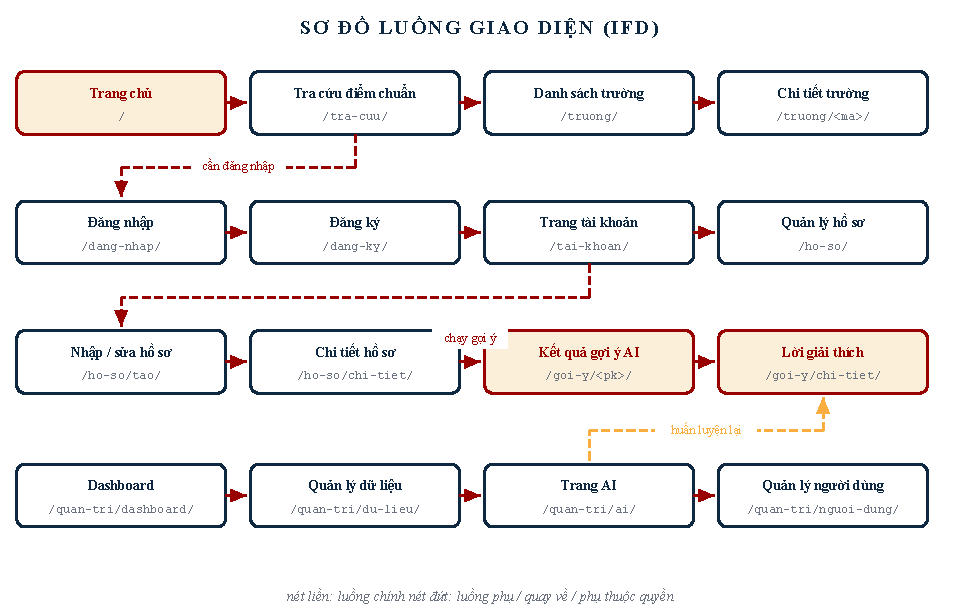
\includegraphics[width=\textwidth]{figs/svg/h-ifd.pdf}
\caption{Sơ đồ luồng giao diện (IFD) của hệ thống Uni Connect.}
\label{fig:ifd}
\end{figure}

Luồng nghiệp vụ trung tâm đi từ màn hình chi tiết hồ sơ sang trang kết quả gợi ý, tại đây hệ thống gọi mô hình để sinh xác suất trúng tuyển và phân tầng kết quả. Từ trang kết quả, học sinh có thể mở trang lời giải thích chi tiết cho từng nguyện vọng, chuyển sang màn hình so sánh nhiều nguyện vọng cạnh nhau, hoặc truy cập lại lịch sử các lần gợi ý trước đó.

\chapter{Cài đặt, thử nghiệm và đánh giá kết quả}
\label{ch:caidat}
\label{ch:ketqua}

Chương này trình bày phần hiện thực của hệ thống Uni Connect: môi trường triển khai,
các thành phần mã nguồn chính, giao diện người dùng thực tế, kết quả kiểm thử và kết
quả thực nghiệm của mô hình học máy. Nội dung chương là căn cứ để đối chiếu bốn mục
tiêu đã đặt ra ở Chương~\ref{ch:modau} với kết quả đo được.

\section{Môi trường triển khai}

Hệ thống được lập trình, huấn luyện và kiểm thử hoàn chỉnh trên môi trường máy chủ
cục bộ với các thông số cấu hình cụ thể:
\begin{itemize}[leftmargin=1.6em, itemsep=2pt]
  \item \textbf{Phần cứng:} Vi xử lý Intel Core i7 12 nhân 16 luồng, bộ nhớ trong RAM 16~GB DDR5, ổ cứng lưu trữ thể rắn NVMe SSD 512~GB.
  \item \textbf{Hệ điều hành:} Microsoft Windows 11 Home 64-bit kết hợp môi trường thực thi POSIX Git Bash.
  \item \textbf{Môi trường runtime:} Python 3.13.2 64-bit, quản lý gói thông qua \code{pip} và môi trường ảo \code{venv}.
  \item \textbf{Cơ sở dữ liệu:} MySQL Server 8.0 Community Edition, bảng mã lưu trữ \code{utf8mb4}.
  \item \textbf{Quản lý phiên bản:} Hệ thống kiểm soát phiên bản Git, lưu trữ kho mã nguồn tại GitHub (\url{https://github.com/tann299/DAU-2026-2027-Uni-Map}).
\end{itemize}

Bảng~\ref{tab:moitruong} đối chiếu cấu hình máy phát triển dùng để huấn luyện với cấu
hình máy chủ tối thiểu mà hệ thống cần để vận hành. Việc tách hai cấu hình này là có
chủ đích: huấn luyện mô hình đòi hỏi nhiều nhân CPU và RAM, trong khi phục vụ trực
tuyến chỉ cần nạp sẵn \code{model.pkl} vào bộ nhớ và trả kết quả cho từng truy vấn.

\begin{table}[H]
\centering
\caption{Đối chiếu cấu hình máy phát triển (huấn luyện) và máy chủ vận hành (phục vụ).}
\label{tab:moitruong}
\small
\begin{tabularx}{\textwidth}{@{}>{\raggedright\arraybackslash}p{3.1cm}
  >{\raggedright\arraybackslash}X
  >{\raggedright\arraybackslash}X@{}}
\toprule
\rowcolor{gray100}\bfseries\color{daunavy}Thành phần &
\bfseries\color{daumaroon}Máy phát triển (huấn luyện) &
\bfseries\color{daunavy}Máy chủ vận hành (tối thiểu) \\
\midrule
CPU        & Intel Core i7, 12 nhân / 16 luồng & 1 vCPU \\
RAM        & 16~GB DDR5                        & 2~GB \\
Lưu trữ    & NVMe SSD 512~GB                   & 20~GB (mã nguồn, CSDL, \code{model.pkl}) \\
Hệ điều hành & Windows 11 Home 64-bit          & Linux (Ubuntu 22.04 LTS) \\
Python     & 3.13.2                            & 3.13.x \\
MySQL      & 8.0 Community, \code{utf8mb4}     & 8.0, \code{utf8mb4} \\
Vai trò    & Chạy \code{crawl}, \code{gen\_dataset}, \code{train} & Chạy Django + Gunicorn, nạp mô hình vào RAM \\
\bottomrule
\end{tabularx}
\end{table}

Bảng~\ref{tab:moitruong} cho thấy toàn bộ yêu cầu tài nguyên của hệ thống nằm trong
ngưỡng một máy chủ VPS phổ thông: 1 vCPU và 2~GB RAM là đủ để phục vụ, vì chi phí
tính toán nặng (sinh đặc trưng, huấn luyện 100 cây) đã được đẩy ra khỏi vòng đời
truy vấn. Ràng buộc thực sự đáng kể là dung lượng RAM dành cho \code{model.pkl}
($\approx$~52~MB) và bộ đệm của MySQL; hai mục này chiếm phần lớn trong 2~GB nêu
trên. Cấu hình phát triển mạnh hơn chỉ cần thiết ở giai đoạn huấn luyện, khi
\code{train.py} chạy song song trên toàn bộ nhân CPU thông qua \code{n\_jobs = -1}.

Hình~\ref{fig:deploy} mô tả cách các thành phần trên được bố trí khi triển khai thật.

\begin{figure}[H]
\centering
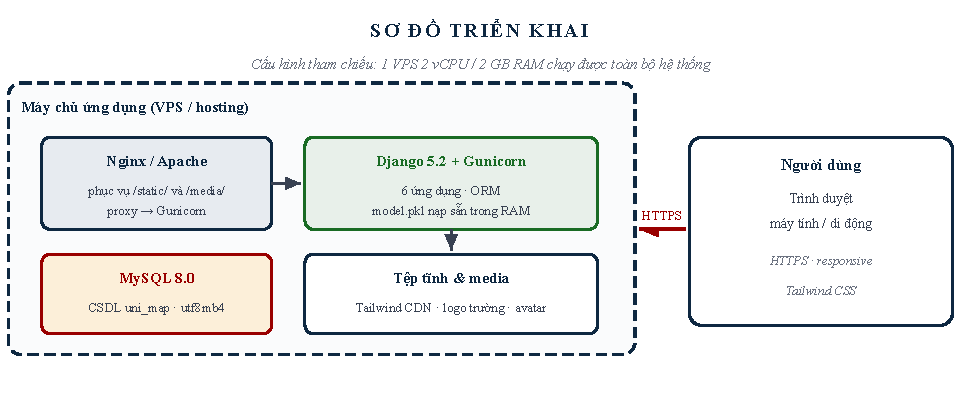
\includegraphics[width=\textwidth]{figs/svg/h-deploy.pdf}
\caption{Sơ đồ triển khai hệ thống trên một máy chủ VPS đơn lẻ.}
\label{fig:deploy}
\end{figure}

Trong Hình~\ref{fig:deploy}, máy chủ đứng sau một lớp Nginx/Apache đóng vai trò phục vụ
tệp tĩnh và chuyển tiếp yêu cầu động sang tiến trình Gunicorn chạy ứng dụng Django.
Tiến trình này nạp sẵn \code{model.pkl} vào RAM ngay khi khởi động, nên mỗi lượt gợi
ý chỉ còn chi phí vector hóa và gọi \code{predict\_proba}. MySQL 8.0 nằm cùng máy chủ
và chỉ được truy cập qua Django ORM; tệp tĩnh và media (logo trường, ảnh đại diện)
được phục vụ trực tiếp, không đi qua tầng ứng dụng. Toàn bộ đường truyền từ trình
duyệt tới máy chủ dùng HTTPS. Cách bố trí một máy chủ này phù hợp với quy mô đồ án,
đồng thời giữ nguyên khả năng tách tầng sau này: nếu lượng truy cập tăng, chỉ cần
chuyển MySQL sang máy riêng và nhân bản tiến trình Gunicorn mà không sửa mã nguồn.

\section{Các thành phần mã nguồn chính}

Kiến trúc mã nguồn được phân rã thành hai phân hệ độc lập: phân hệ xử lý dữ liệu
ngoại tuyến (\en{offline pipeline}) và phân hệ ứng dụng web trực tuyến
(\en{online service}). Hình~\ref{fig:pipeline} tóm tắt toàn bộ đường đi của dữ liệu
qua sáu bước của phân hệ ngoại tuyến.

\begin{figure}[H]
\centering
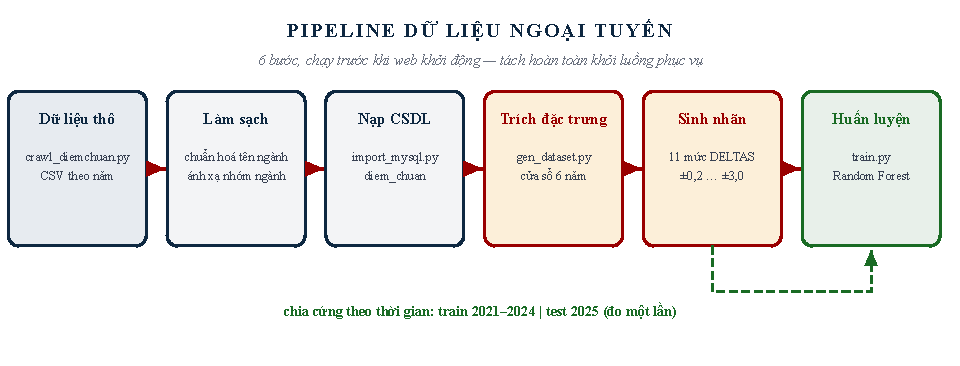
\includegraphics[width=\textwidth]{figs/svg/h-pipeline.pdf}
\caption{Pipeline dữ liệu ngoại tuyến gồm sáu bước, chạy trước khi web khởi động.}
\label{fig:pipeline}
\end{figure}

Sáu bước trong Hình~\ref{fig:pipeline} tương ứng sáu tệp mã nguồn độc lập, mỗi bước
ghi ra một đầu ra trung gian kiểm tra được. Bước 1 (\code{crawl\_diemchuan.py}) sinh
ra các tệp CSV theo năm; bước 2 làm sạch tên ngành và ánh xạ về 15 nhóm ngành chuẩn;
bước 3 nạp vào MySQL qua \code{import\_mysql.py}; bước 4 (\code{gen\_dataset.py})
trích đặc trưng từ cửa sổ sáu năm; bước 5 sinh nhãn bằng 11 mức \code{DELTAS}; bước 6
(\code{train.py}) huấn luyện và đóng gói mô hình. Điểm quan trọng là ranh giới thời
gian: dữ liệu được chia cứng thành tập huấn luyện 2021--2024 và tập kiểm thử 2025, và
phép chia này chỉ thực hiện đúng một lần để kết quả đo không bị nhiễu bởi việc chọn
lại tập kiểm thử.

\subsection{Pipeline tiền xử lý và sinh tập dữ liệu}

Module \code{gen\_dataset.py} thực hiện chuyển đổi chuỗi 10 năm điểm chuẩn từ bảng
quan hệ thành tập dữ liệu huấn luyện phẳng. Để ngăn chặn hoàn toàn rò rỉ dữ liệu, hàm
xử lý tính toán đặc trưng tại năm $t$ chỉ dựa trên cửa sổ lịch sử 6 năm trước đó
($t - \text{lookback} \le \text{năm} < t$) và áp dụng 11 mức chênh lệch điểm đối xứng
\code{DELTAS} để sinh mẫu thí sinh giả lập.

\begin{lstlisting}[language=Python, caption={Hàm sinh mẫu giả lập đối xứng và tách tập theo thời gian.}, label={lst:gendata}]
# Symmetric delta grid around true cutoff score (constants.py)
DELTAS = [-3.0, -2.0, -1.0, -0.5, -0.2, 0.0, 0.2, 0.5, 1.0, 2.0, 3.0]
NAM_LOOKBACK = 6

def build_split(df_history, target_year):
    """Generate training rows for target_year using only years < target_year."""
    valid_window = [y for y in range(target_year - NAM_LOOKBACK, target_year)]
    features = extract_window_features(df_history, valid_window)

    # Expand each application row across 11 synthetic candidates
    expanded_rows = []
    for _, row in features.iterrows():
        cutoff = row["diem_chuan_target"]
        for d in DELTAS:
            sim_score = cutoff + d
            label = 1 if sim_score >= cutoff else 0
            expanded_rows.append({
                **row.to_dict(),
                "diem_thi": sim_score,
                "margin": d,
                "nhan": label
            })
    return pd.DataFrame(expanded_rows)
\end{lstlisting}

Mã nguồn~\ref{lst:gendata} cho thấy hai quyết định kỹ thuật được thể hiện trực tiếp
trong vòng lặp. Thứ nhất, \code{valid\_window} bị chặn trên bởi \code{target\_year}
nên không một giá trị nào của năm mục tiêu lọt vào vector đặc trưng. Thứ hai, nhãn
được suy ra từ chính \code{cutoff} của năm mục tiêu chứ không từ dữ liệu quá khứ, nên
nhãn và đặc trưng nằm ở hai mốc thời gian khác nhau đúng như thiết kế. Mỗi dòng lịch
sử được nhân thành 11 dòng huấn luyện, nhờ đó tỉ lệ hai lớp gần cân bằng mà không cần
kỹ thuật lấy mẫu bù.

\subsection{Huấn luyện mô hình và tối ưu kích thước lưu trữ}

Quy trình huấn luyện trong \code{train.py} thực hiện chuẩn hóa dữ liệu bằng
\code{StandardScaler} và huấn luyện mô hình \code{RandomForestClassifier}. Để đáp ứng
ràng buộc lưu trữ dưới 100~MB (nhằm đưa vào bộ nhớ RAM máy chủ phổ thông), số lượng
cây được chốt ở 100 và độ sâu tối đa được giới hạn ở mức 14.

\begin{lstlisting}[language=Python, caption={Quy trình huấn luyện và đóng gói mô hình.}, label={lst:train}]
from sklearn.ensemble import RandomForestClassifier
from sklearn.preprocessing import StandardScaler
import joblib

def train_and_export(X_train, y_train, export_dir="ml/"):
    """Fit scaler and Random Forest model, then export serialized weights."""
    scaler = StandardScaler().fit(X_train)
    Z_train = scaler.transform(X_train)

    # 100 estimators, max depth 14 limits pkl file size to ~52 MB
    rf = RandomForestClassifier(
        n_estimators=100,
        min_samples_leaf=5,
        max_depth=14,
        n_jobs=-1,
        random_state=42
    )
    rf.fit(Z_train, y_train)

    joblib.dump(rf, f"{export_dir}/model.pkl", compress=3)
    joblib.dump(scaler, f"{export_dir}/scaler.pkl")
    return rf, scaler
\end{lstlisting}

Điểm đáng chú ý trong Mã nguồn~\ref{lst:train} là bộ chuẩn hóa \code{scaler} được lưu
thành một tệp riêng thay vì gộp vào mô hình. Khi suy luận, ứng dụng web phải nạp lại
đúng bộ chuẩn hóa này để biến đổi vector đầu vào theo cùng tham số trung bình và độ
lệch chuẩn đã dùng lúc huấn luyện; nếu thiếu bước đó, \code{StandardScaler} sẽ dùng
tham số mặc định và toàn bộ dự đoán sai lệch. Tham số \code{compress=3} của
\code{joblib} giảm kích thước tệp còn khoảng 52~MB mà thời gian nạp vẫn dưới một giây,
phù hợp với yêu cầu nạp một lần lúc khởi động.

\subsection{Động cơ suy luận và cơ chế chịu lỗi}

Tại tầng ứng dụng web Django, tệp \code{predict.py} nạp mô hình vào bộ nhớ RAM dưới
dạng biến toàn cục để tránh chi phí I/O đọc đĩa cứng trong mỗi lượt truy vấn của
người dùng. Khi nhận danh sách các ngành ứng viên, mô hình thực hiện dự đoán theo lô
(\en{batch prediction}) bằng phương thức \code{predict\_proba}, đảm bảo thời gian xử
lý toàn bộ 30 nguyện vọng dưới 50 mili-giây.

\begin{lstlisting}[language=Python, caption={Hàm chấm xác suất theo lô và cơ chế dự phòng.}, label={lst:predict}]
_CACHE = {"model": None, "scaler": None}

def cham_xac_suat(ds_nguyen_vong, diem_thi):
    """Batch inference with graceful fallback to margin ranking."""
    try:
        if _CACHE["model"] is None:
            _CACHE["model"] = joblib.load("ml/model.pkl")
            _CACHE["scaler"] = joblib.load("ml/scaler.pkl")

        # Build 27-dim feature matrix Z for all candidates at once
        X = vector_hoa_hang_loat(ds_nguyen_vong, diem_thi)
        Z = _CACHE["scaler"].transform(X)
        probs = _CACHE["model"].predict_proba(Z)[:, 1]
        return probs, "AI_RANDOM_FOREST"
    except Exception as e:
        # Fallback to deterministic margin sorting when model fails
        margins = [diem_thi - nv["diem_moi_nhat"] for nv in ds_nguyen_vong]
        return margins, "FALLBACK_MARGIN"
\end{lstlisting}

Mã nguồn~\ref{lst:predict} là hiện thực của yêu cầu phi chức năng về độ tin cậy: khối
\code{try} bao trọn cả bước nạp mô hình, vector hóa và suy luận, nên mọi sự cố (thiếu
tệp, sai phiên bản thư viện, lỗi định dạng) đều rơi vào cùng một nhánh xử lý. Nhánh
\code{except} không trả về lỗi mà chuyển sang xếp hạng theo \code{margin} thuần và
đánh dấu nguồn kết quả là \code{FALLBACK\_MARGIN}; nhãn này được truyền xuống giao
diện để người dùng biết kết quả hiện tại không đến từ mô hình AI. Nhờ vậy hệ thống
luôn trả về mã HTTP 200 kèm một danh sách gợi ý hợp lệ, đúng với cam kết ở
Mục~\ref{sec:nfr}.

\section{Giao diện và kịch bản sử dụng}

Ứng dụng web được xây dựng với phong cách trực quan, tối ưu cho cả máy tính để bàn và
thiết bị di động bằng framework Tailwind CSS. Cấu trúc trang được bố trí gồm 4 phân
khu chính:

\begin{enumerate}[leftmargin=1.6em, itemsep=2pt]
  \item \textbf{Trang tra cứu thông tin trường và ngành:} Cho phép lọc nhanh 295 trường theo 3 vùng miền, loại hình công lập/tư thục và xem chuỗi 10 năm điểm chuẩn trực quan (Hình~\ref{fig:demo-tracuu}).
  \item \textbf{Trang quản lý hồ sơ điểm cá nhân:} Thí sinh nhập điểm các môn thi THPT hoặc điểm học bạ lớp 12. Hệ thống tự động tính toán tổng điểm cho tất cả các tổ hợp xét tuyển hợp lệ (Hình~\ref{fig:demo-hoso}).
  \item \textbf{Trang gợi ý nguyện vọng AI:} Hiển thị danh sách nguyện vọng được sắp xếp theo xác suất giảm dần và phân thành 3 khối màu rõ rệt: Tầng \textbf{An toàn} (màu xanh lá, $p \ge 0{,}80$), Tầng \textbf{Vừa sức} (màu xanh dương, $0{,}40 \le p < 0{,}80$) và Tầng \textbf{Thử sức} (màu cam, $p < 0{,}40$). Mỗi hàng đi kèm thẻ giải thích nguyên nhân ngắn gọn. Giao diện thực tế của trang này thể hiện ở Hình~\ref{fig:demo-goiy}.
  \item \textbf{Trang quản trị hệ thống:} Dành cho quản trị viên theo dõi số lượng bản ghi dữ liệu, kích hoạt pipeline chạy ngầm cập nhật dữ liệu và thực hiện huấn luyện lại mô hình trực tiếp trên giao diện (Hình~\ref{fig:demo-admin}).
\end{enumerate}

\begin{figure}[H]
\centering
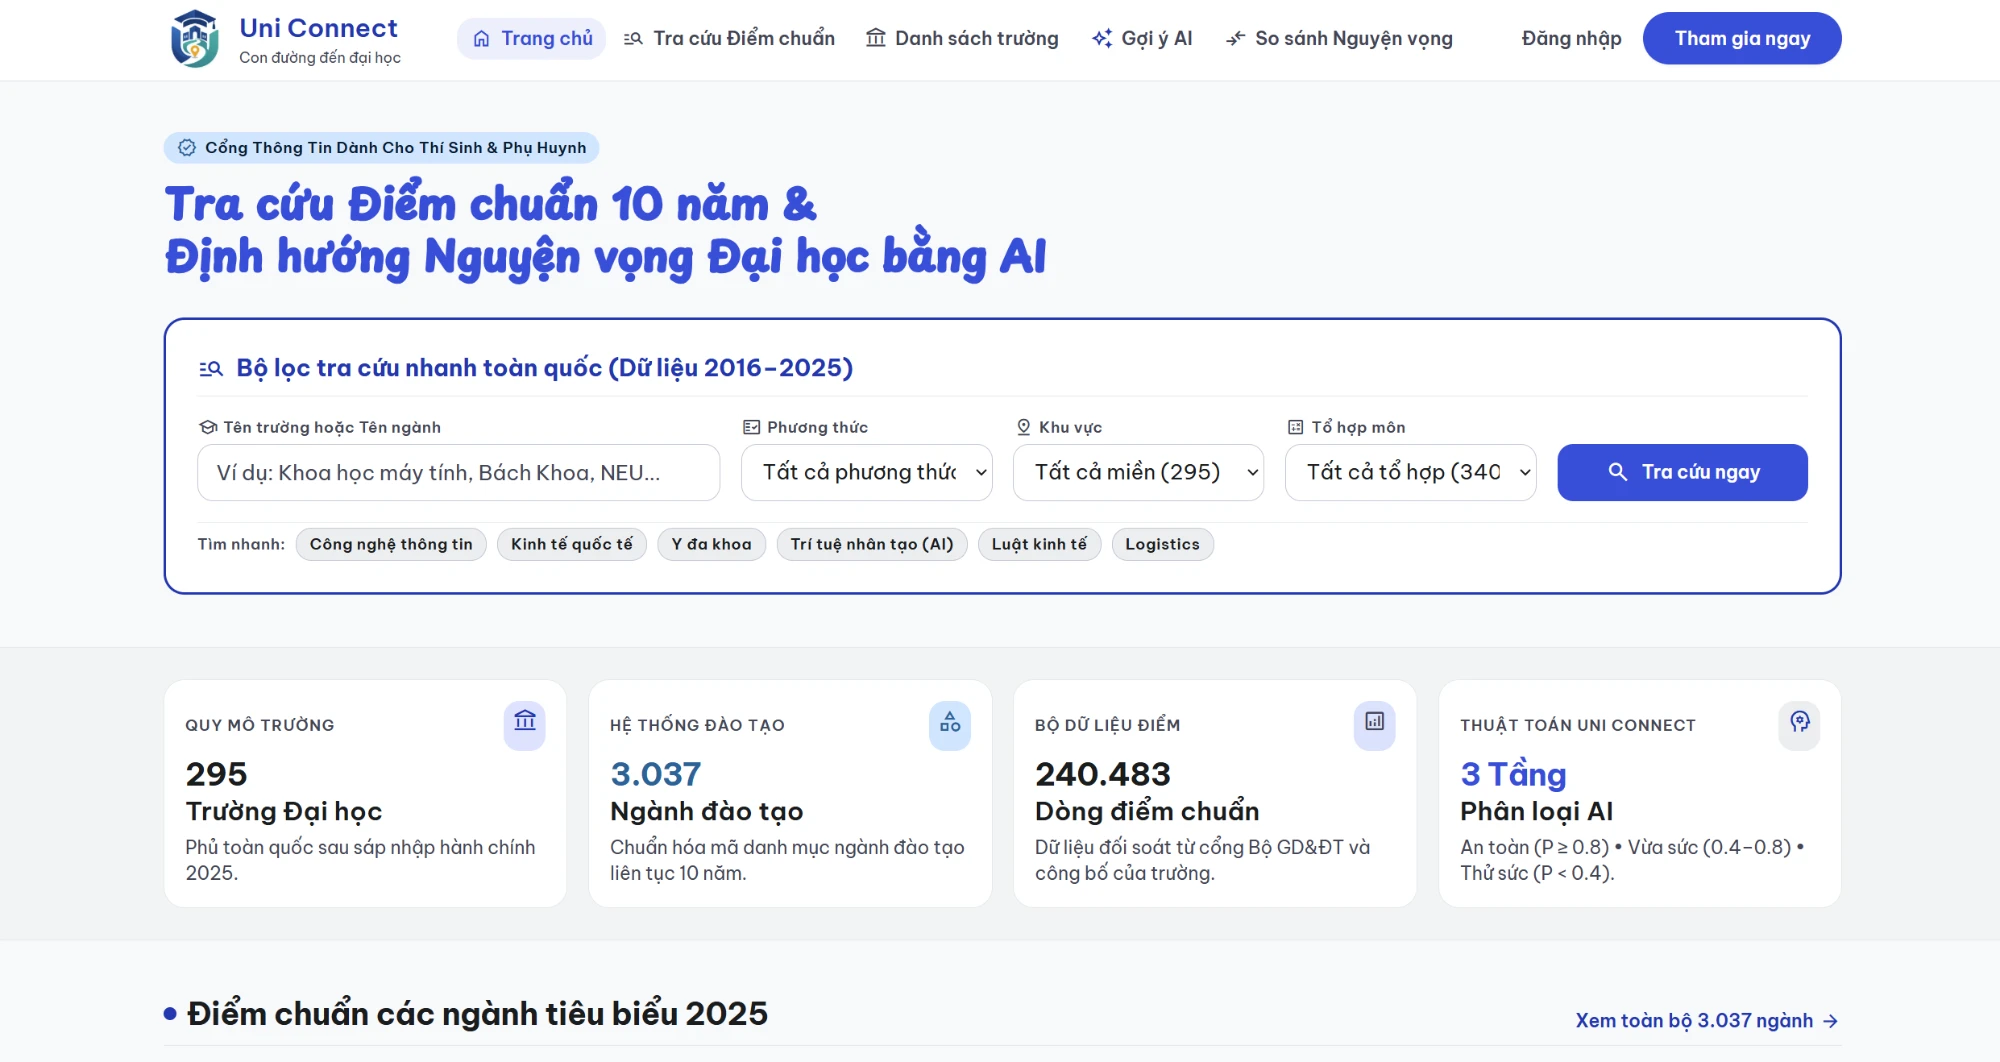
\includegraphics[width=\textwidth]{figs/uniconnect-p1.png}
\caption{Giao diện trang chủ Uni Connect --- tra cứu điểm chuẩn 10 năm.}
\label{fig:demo-tracuu}
\end{figure}

Hình~\ref{fig:demo-tracuu} là trang chủ của hệ thống. Phần đầu trang đặt ô tìm kiếm
theo tên trường, ngành hoặc mã trường kèm bốn bộ lọc (tỉnh thành, tổ hợp môn, nhóm
ngành, phương thức). Bên dưới là bốn ô thống kê lấy trực tiếp từ cơ sở dữ liệu: 295
trường, 3.037 ngành, 240.483 dòng điểm và 3 tầng gợi ý. Bảng điểm chuẩn ở cuối trang
hiển thị song song ba năm gần nhất cùng cột biến động, cho phép người dùng nhận ra xu
hướng tăng giảm ngay ở màn hình đầu tiên mà không phải mở trang chi tiết.

\begin{figure}[H]
\centering
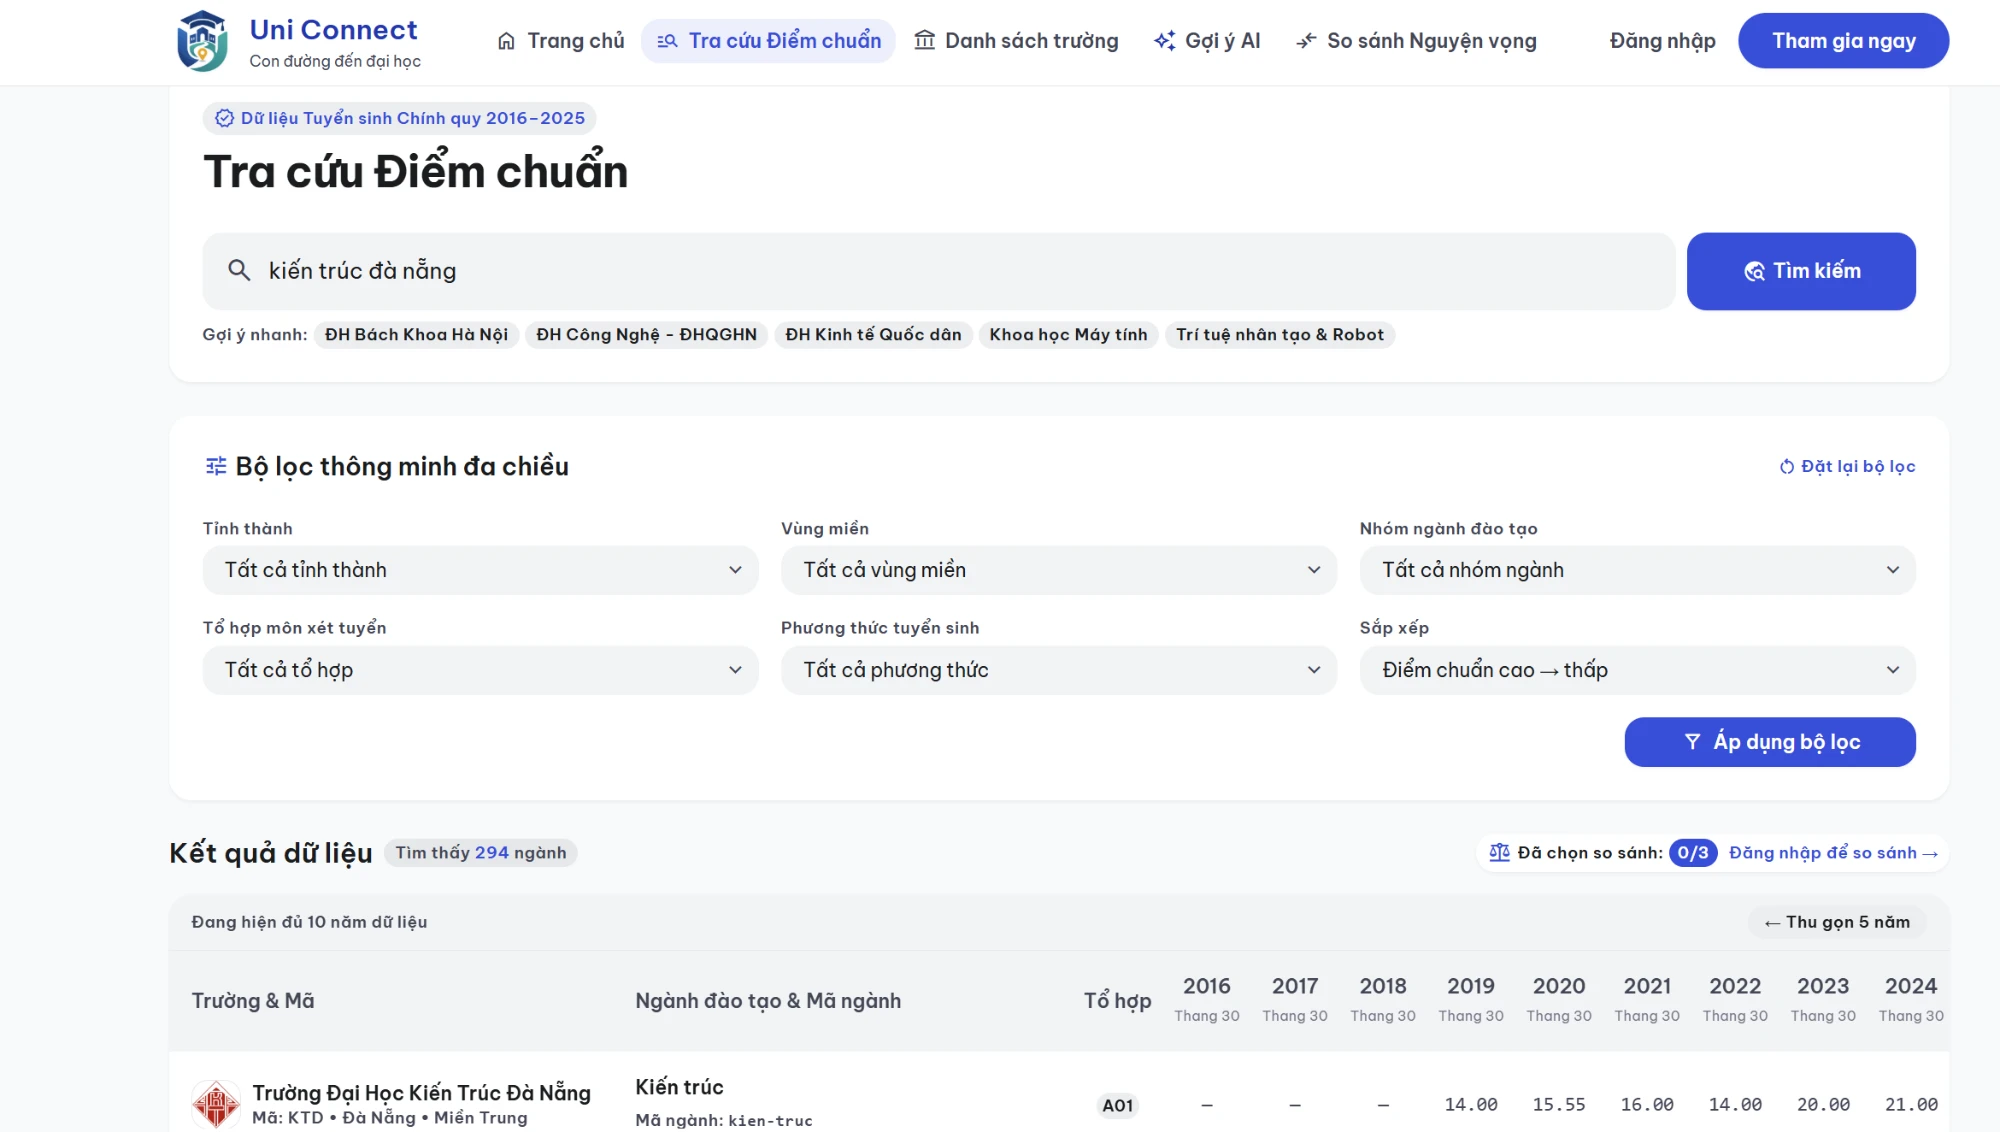
\includegraphics[width=\textwidth]{figs/uniconnect-p2.png}
\caption{Giao diện trang tra cứu điểm chuẩn đa tiêu chí.}
\label{fig:demo-hoso}
\end{figure}

Hình~\ref{fig:demo-hoso} là trang tra cứu chi tiết. Mỗi dòng kết quả gồm tên trường,
mã trường, tên ngành, tổ hợp xét tuyển và chuỗi điểm của các năm. Cột ngoài cùng bên
phải gắn nhãn xu hướng (tăng, giảm, ổn định) được tính từ hồi quy tuyến tính trên
chuỗi điểm, giúp thí sinh so sánh nhanh mức độ cạnh tranh giữa các ngành thay vì chỉ
nhìn một con số của năm gần nhất.

\begin{figure}[H]
\centering
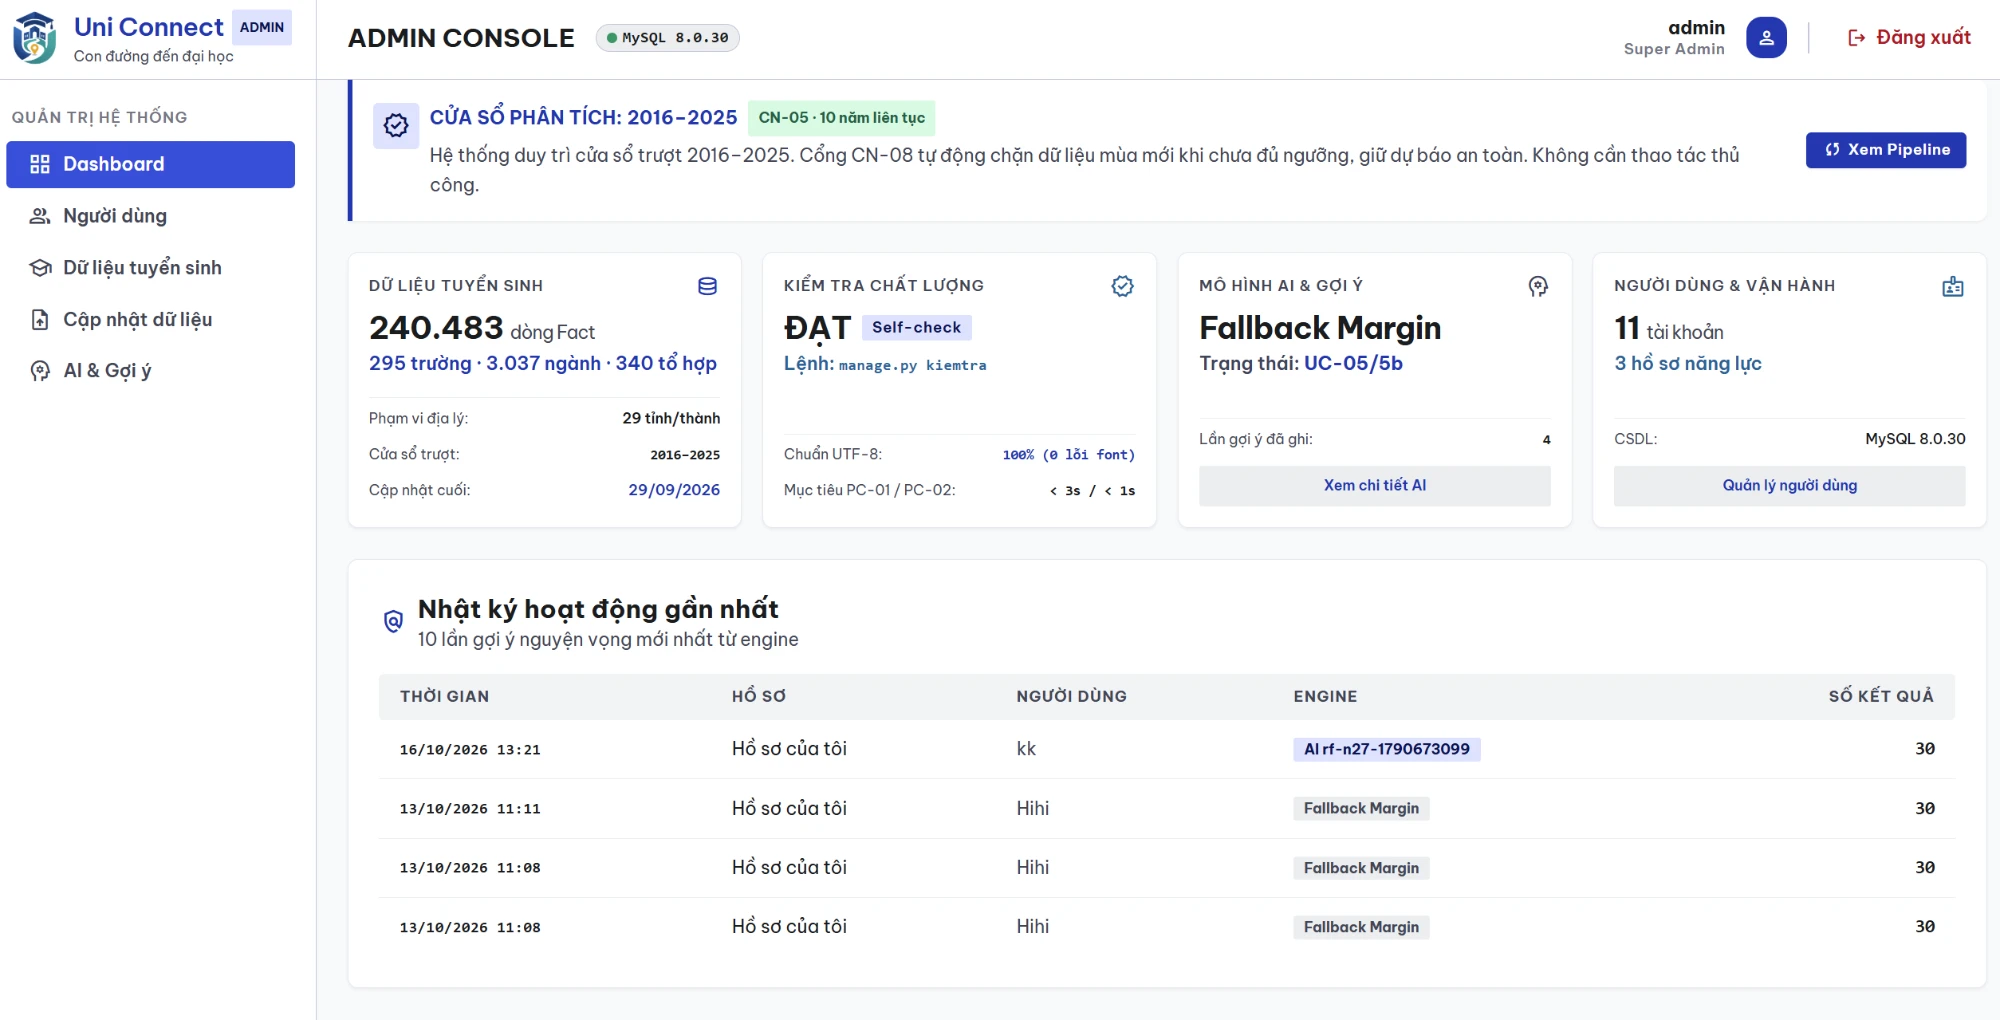
\includegraphics[width=\textwidth]{figs/uniconnect-p4.png}
\caption{Giao diện bảng điều khiển quản trị hệ thống (Admin Console).}
\label{fig:demo-admin}
\end{figure}

Hình~\ref{fig:demo-admin} là bảng điều khiển dành cho quản trị viên. Bốn thẻ đầu trang
tổng hợp trạng thái hệ thống: số dòng dữ liệu, kết quả tự kiểm tra chất lượng, trạng
thái mô hình AI và thông tin người dùng. Bảng nhật ký phía dưới ghi lại từng lần chạy
gợi ý kèm nguồn xử lý (\code{AI\_RANDOM\_FOREST} hoặc \code{FALLBACK\_MARGIN}), nhờ
đó có thể phát hiện ngay nếu mô hình gặp sự cố trong vận hành thực tế.

\begin{figure}[H]
\centering
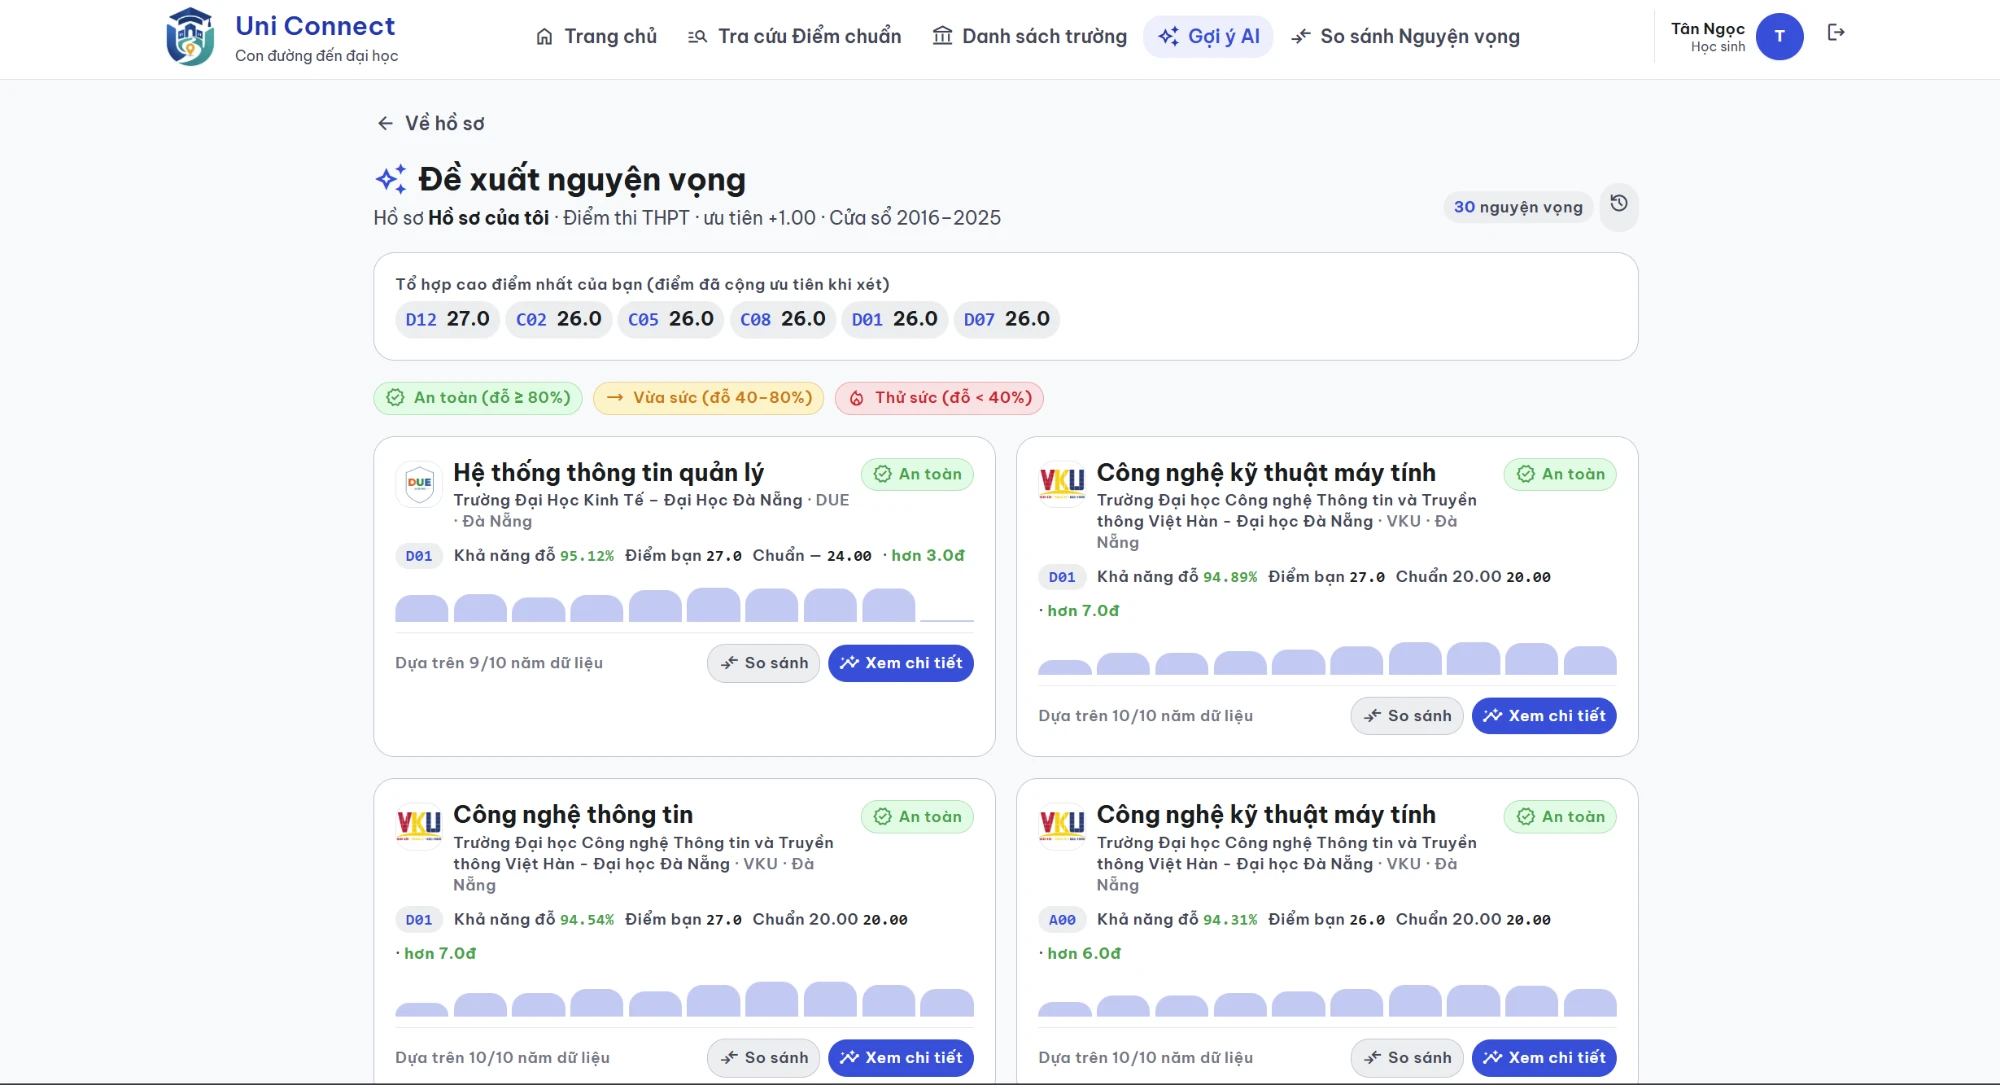
\includegraphics[width=\textwidth]{figs/uniconnect-goiy.png}
\caption{Giao diện trang gợi ý nguyện vọng AI với phân tầng An toàn, Vừa sức, Thử sức.}
\label{fig:demo-goiy}
\end{figure}

Hình~\ref{fig:demo-goiy} là màn hình trung tâm của hệ thống. Ba tab ở đầu trang tương
ứng ba tầng và ghi rõ ngưỡng xác suất ngay trên nhãn, nên người dùng không phải tự
đoán ý nghĩa màu sắc. Mỗi thẻ nguyện vọng hiển thị tên ngành, trường, tổ hợp, khả
năng đỗ, điểm của bản thân so với điểm chuẩn mới nhất, giá trị \code{margin} và đồ thị
chuỗi 10 năm. Những con số này chính là đầu vào của mô hình, được hiển thị lại để lời
gợi ý có thể kiểm chứng được thay vì là một kết quả hộp đen.

\section{Kiểm thử hệ thống}

Chất lượng và độ ổn định của hệ thống được kiểm chứng qua ba cấp độ kiểm thử: kiểm
thử đơn vị (\en{unit test}), kiểm thử tích hợp (\en{integration test}) và kiểm thử
khả năng chịu lỗi (\en{fault tolerance}). Hình~\ref{fig:testing} mô tả phạm vi của
từng cấp độ.

\begin{figure}[H]
\centering
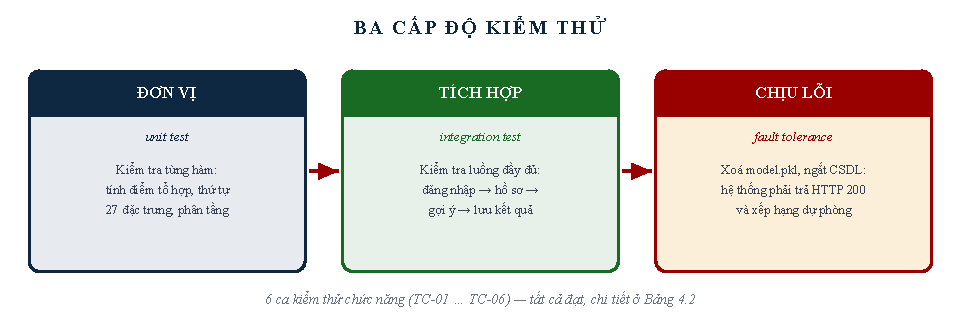
\includegraphics[width=\textwidth]{figs/svg/h-testing.pdf}
\caption{Ba cấp độ kiểm thử áp dụng cho hệ thống Uni Connect.}
\label{fig:testing}
\end{figure}

Ba cấp độ trong Hình~\ref{fig:testing} được thiết kế để phủ những rủi ro khác nhau.
Kiểm thử đơn vị kiểm tra từng hàm thuần túy --- tính tổng điểm tổ hợp, thứ tự 27 đặc
trưng, quy tắc gán tầng --- nơi lỗi thường là lỗi công thức và dễ tái hiện. Kiểm thử
tích hợp đi theo một luồng đầy đủ từ đăng nhập, nhập hồ sơ, gọi gợi ý đến lưu kết quả,
nhằm bắt lỗi ở các điểm nối giữa các tầng. Kiểm thử chịu lỗi cố tình phá vỡ điều kiện
bình thường (xóa \code{model.pkl}, ngắt kết nối CSDL) để xác nhận hệ thống vẫn trả về
mã HTTP 200 cùng kết quả dự phòng thay vì sập.

\begin{table}[H]
\centering
\caption{Kịch bản và kết quả các ca kiểm thử chính của hệ thống Uni Connect.}
\label{tab:kiemthu}
\small
\begin{tabularx}{\textwidth}{@{}>{\bfseries\color{daunavy}\raggedright\arraybackslash}m{2.45cm}
  >{\raggedright\arraybackslash}X
  >{\raggedright\arraybackslash}X
  >{\centering\arraybackslash}m{1.75cm}@{}}
\toprule
\rowcolor{gray100}\bfseries\color{daunavy}Mã kiểm thử & \bfseries\color{daunavy}Mục đích kiểm tra & \bfseries\color{daunavy}Kết quả kỳ vọng & \bfseries\color{daumaroon}Trạng thái \\
\midrule
TC-01 & Kiểm tra tính toán tổng điểm tổ hợp & Điểm cộng chính xác từng môn, đúng công thức hệ số & Đạt \\
TC-02 & Kiểm tra tính nhất quán 27 đặc trưng & Thứ tự cột vector khớp tuyệt đối với file \code{constants.py} & Đạt \\
TC-03 & Kiểm tra suy luận hàng loạt & Đầu ra đủ xác suất cho $N$ nguyện vọng, $0 \le p \le 1$ & Đạt \\
TC-04 & Kiểm tra phân tầng xác suất & Gán đúng 3 nhãn An toàn, Vừa sức, Thử sức theo ngưỡng & Đạt \\
TC-05 & Thử nghiệm khi thiếu file \code{model.pkl} & Chuyển sang xếp hạng \code{margin}, mã HTTP 200, không bị lỗi 500 & Đạt \\
TC-06 & Kiểm tra thời gian đáp ứng (PC-01) & Thời gian trả lời toàn bộ trang gợi ý dưới 3 giây; đo thực tế 0,42 giây & Đạt \\
\bottomrule
\end{tabularx}
\end{table}

Bảng~\ref{tab:kiemthu} tổng hợp kết quả của sáu ca kiểm thử chức năng, mỗi ca tương
ứng một rủi ro cụ thể. TC-01 và TC-02 bảo vệ tính đúng đắn của dữ liệu đầu vào mô
hình: một sai lệch thứ tự cột sẽ khiến mô hình nhận nhầm đặc trưng và cho ra xác suất
vô nghĩa dù không hề báo lỗi. TC-03 và TC-04 kiểm tra đầu ra, bảo đảm mọi giá trị xác
suất nằm trong $[0, 1]$ và nhãn tầng được gán đúng theo ngưỡng công bố. TC-05 là ca
quan trọng nhất về mặt vận hành: khi cố tình xóa tệp nhị phân của mô hình, hệ thống
không làm gián đoạn trải nghiệm người dùng mà ngay lập tức trả về danh sách sắp xếp
theo khoảng cách điểm kèm thông báo giải thích rõ ràng. TC-06 xác nhận chỉ tiêu hiệu
năng PC-01 với thời gian đo thực tế 0,42 giây, thấp hơn ngưỡng 3 giây gần bảy lần.

\section{Kết quả đạt được}

Bảng~\ref{tab:muctieu} đối chiếu trực tiếp bốn mục tiêu nêu tại
Chương~\ref{ch:modau} với kết quả đo được và ngưỡng đã cam kết.

\begin{table}[H]
\centering
\caption{Đối chiếu mục tiêu đặt ra với kết quả thực tế của đồ án.}
\label{tab:muctieu}
\small
\begin{tabularx}{\textwidth}{@{}>{\raggedright\arraybackslash}p{2.6cm}
  >{\raggedright\arraybackslash}p{3.5cm}
  >{\raggedright\arraybackslash}X
  >{\centering\arraybackslash}p{1.9cm}@{}}
\toprule
\rowcolor{gray100}\bfseries\color{daunavy}Mục tiêu &
\bfseries\color{daunavy}Ngưỡng đề ra &
\bfseries\color{daumaroon}Kết quả đo được &
\bfseries\color{daunavy}Đánh giá \\
\midrule
1. Dữ liệu & $\ge$ 250 trường; $\ge$ 3.000 ngành; $\ge$ 200.000 bản ghi &
295 trường; 3.037 ngành; 240.483 bản ghi điểm chuẩn 10 năm (2016--2025) &
Vượt mức \\
\addlinespace[2pt]
2. Mô hình AI & Accuracy $>$ 70\%; ROC-AUC $>$ 0,80 &
Accuracy 74,56\%; ROC-AUC 0,8354 trên tập kiểm thử độc lập 2025 &
Đạt \\
\addlinespace[2pt]
3. Phân tầng và giải thích & 3 tầng theo $p$; mỗi gợi ý có lời giải thích &
Ba tầng 0,80 / 0,40 vận hành ổn định; lời giải thích sinh từ \code{margin}, \code{xu_huong}, \code{bien_dong} &
Đạt \\
\addlinespace[2pt]
4. Ứng dụng web & Django $+$ MySQL; phản hồi $<$ 3 giây &
Đủ bốn phân khu chức năng; thời gian phản hồi đo được 0,42 giây &
Đạt \\
\bottomrule
\end{tabularx}
\end{table}

Bảng~\ref{tab:muctieu} cho thấy cả bốn mục tiêu đều đạt hoặc vượt ngưỡng. Mục tiêu dữ
liệu vượt ở cả ba chỉ số, chủ yếu nhờ quá trình thu thập kéo dài trọn 10 năm thay vì
chỉ lấy vài năm gần nhất. Ba mục tiêu còn lại đều đạt với khoảng dự phòng đáng kể:
Accuracy vượt ngưỡng gần 4,6 điểm phần trăm, ROC-AUC vượt 0,035 và thời gian phản hồi
thấp hơn ngưỡng gần bảy lần. Khoảng dự phòng này là cần thiết vì các phép đo được thực
hiện trên một máy chủ cục bộ; khi triển khai thật, độ trễ mạng và tải đồng thời sẽ ăn
bớt một phần lợi thế đó.

\section{Độ đo đánh giá}

Thực nghiệm đo duy nhất một lần trên tập kiểm thử độc lập năm 2025 gồm 244.123 mẫu
(tập huấn luyện 2021--2024 gồm 913.924 mẫu), giữ nguyên siêu tham số chốt tại
Chương~\ref{ch:thietke}. Bảng~\ref{tab:ketqua} so sánh mô hình chính với mô hình đối
chứng.

\begin{table}[H]
\centering
\caption{So sánh Decision Tree và Random Forest trên tập kiểm thử năm 2025 (244.123 mẫu).}
\label{tab:ketqua}
\resizebox{\textwidth}{!}{%
\begin{tabular*}{\textwidth}{@{\extracolsep{\fill}}>{\bfseries\color{daunavy}}l cccc}
\toprule
\rowcolor{gray100}\bfseries\color{daunavy}Mô hình & \bfseries\color{daumaroon}Accuracy & \bfseries\color{daumaroon}ROC-AUC & \bfseries\color{daumaroon}Brier $\downarrow$ & \bfseries\color{daumaroon}F1 (lớp Đỗ) \\
\midrule
Decision Tree (đối chứng) & 0,7214 & 0,7535 & 0,2550 & 0,7183 \\
Random Forest (chính)     & \textbf{0,7456} & \textbf{0,8354} & \textbf{0,1763} & \textbf{0,7493} \\
\bottomrule
\end{tabular*}}
\end{table}

Bảng~\ref{tab:ketqua} là kết quả trung tâm của đồ án. Hai mô hình dùng chung tập huấn
luyện, chung bộ 27 đặc trưng và chung \code{min\_samples\_leaf = 5}, nên khác biệt duy
nhất giữa chúng là cơ chế tập hợp của Random Forest; mọi chênh lệch đo được vì thế
quy về đúng kỹ thuật bagging. Random Forest thắng ở cả bốn chỉ số, trong đó mức cải
thiện lớn nhất nằm ở ROC-AUC và Brier --- hai chỉ số đo chất lượng của giá trị xác
suất chứ không chỉ nhãn cứng.

Hình~\ref{fig:model-bars} trực quan hóa cùng bộ số liệu này để thấy rõ khoảng cách
giữa hai mô hình ở từng chỉ số.

\begin{figure}[H]
\centering
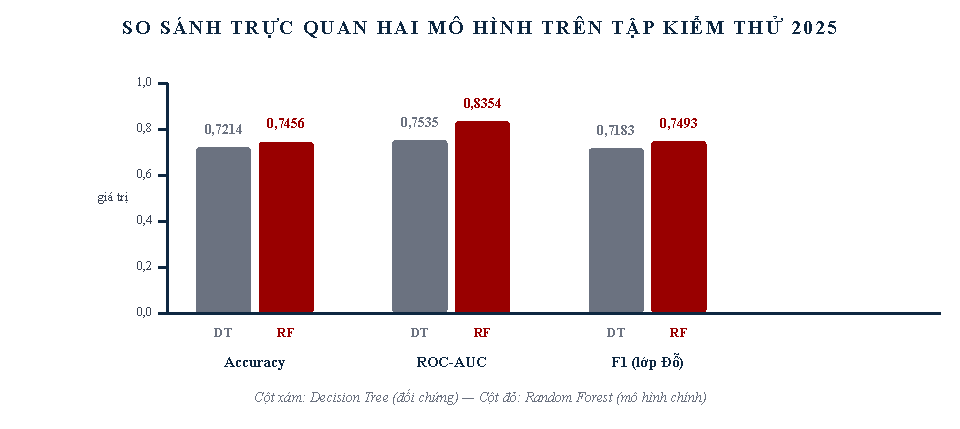
\includegraphics[width=0.92\textwidth]{figs/svg/h-model-bars.pdf}
\caption{So sánh trực quan bốn chỉ số của Decision Tree và Random Forest trên tập kiểm thử 2025.}
\label{fig:model-bars}
\end{figure}

Trong Hình~\ref{fig:model-bars}, cột xám là mô hình đối chứng và cột đỏ là mô hình
chính. Ba nhóm đầu (Accuracy, ROC-AUC, F1) đều là chỉ số ``càng cao càng tốt'' nên
cột đỏ đứng cao hơn là dấu hiệu tích cực. Riêng Brier là chỉ số ``càng thấp càng
tốt'', nên cột đỏ thấp hơn mới là kết quả mong muốn; khoảng cách ở nhóm này lớn hơn
hẳn ba nhóm còn lại, cho thấy lợi ích của Random Forest tập trung vào độ hiệu chuẩn
xác suất.

Bảng~\ref{tab:chi-tiet-lop} đi sâu vào từng lớp dự đoán, vì Accuracy tổng thể có thể
che khuất sự đánh đổi giữa hai loại lỗi.

\begin{table}[H]
\centering
\caption{Chi tiết Precision và Recall theo từng lớp của hai mô hình trên tập kiểm thử 2025.}
\label{tab:chi-tiet-lop}
\small
\begin{tabularx}{\textwidth}{@{}>{\raggedright\arraybackslash}p{3.5cm}
  >{\centering\arraybackslash}p{2.4cm}
  >{\centering\arraybackslash}p{2.4cm}
  >{\centering\arraybackslash}p{2.4cm}
  >{\centering\arraybackslash}p{2.4cm}@{}}
\toprule
\rowcolor{gray100}\bfseries\color{daunavy}Mô hình / Lớp &
\bfseries\color{daumaroon}Precision &
\bfseries\color{daumaroon}Recall &
\bfseries\color{daunavy}Precision &
\bfseries\color{daunavy}Recall \\
\midrule
 & \multicolumn{2}{c}{\bfseries\color{daumaroon}Lớp Đỗ} & \multicolumn{2}{c}{\bfseries\color{daunavy}Lớp Trượt} \\
\midrule
Decision Tree (đối chứng) & 0,8006 & 0,6514 & 0,6581 & 0,8053 \\
Random Forest (chính)     & \textbf{0,8098} & \textbf{0,6973} & \textbf{0,6887} & 0,8035 \\
\bottomrule
\end{tabularx}
\end{table}

Bảng~\ref{tab:chi-tiet-lop} giải thích vì sao Accuracy chỉ tăng 2,42 điểm phần trăm
trong khi ROC-AUC tăng tới 8,19 điểm. Với lớp Đỗ, Random Forest tăng đồng thời cả
Precision (0,8006 lên 0,8098) và Recall (0,6514 lên 0,6973), tức là vừa báo đúng hơn
vừa bỏ sót ít hơn. Với lớp Trượt, Precision tăng từ 0,6581 lên 0,6887 còn Recall gần
như giữ nguyên (0,8053 xuống 0,8035). Cách đánh đổi này phù hợp với mục đích sử dụng:
hệ thống cần hạn chế việc báo nhầm một nguyện vọng là ``an toàn'' khi thực tế rủi ro,
nên ưu tiên Precision của lớp Trượt, trong khi vẫn không đánh mất khả năng cảnh báo.

Ba điểm đọc quan trọng từ hai bảng trên:
\begin{itemize}[leftmargin=1.6em, itemsep=2pt]
  \item \textbf{ROC-AUC tăng 0,0819} (0,7535 $\rightarrow$ 0,8354): khả năng xếp hạng Đỗ/Trượt cải thiện rõ rệt nhờ trung bình 100 cây thay vì một cây đơn.
  \item \textbf{Brier giảm 0,0787} (0,2550 $\rightarrow$ 0,1763): xác suất dự đoán hiệu chuẩn tốt hơn, quan trọng vì hệ thống dùng giá trị $p$ trực tiếp để phân tầng.
  \item \textbf{Recall lớp Đỗ tăng 0,0459} trong khi Recall lớp Trượt giữ nguyên ($\approx$ 0,80): mô hình chính bắt được nhiều cơ hội đỗ hơn mà không đánh đổi khả năng cảnh báo trượt.
\end{itemize}

\subsection{Tầm quan trọng đặc trưng}

Bảng~\ref{tab:fi} trích 6 đặc trưng đóng góp lớn nhất từ \code{feature\_importances\_}
của Random Forest.

\begin{table}[H]
\centering
\caption{Mức đóng góp của 6 đặc trưng quan trọng nhất.}
\label{tab:fi}
\resizebox{0.85\textwidth}{!}{%
\begin{tabular*}{\textwidth}{@{\extracolsep{\fill}}>{\bfseries\color{daunavy}}l c l}
\toprule
\rowcolor{gray100}\bfseries\color{daunavy}Đặc trưng & \bfseries\color{daumaroon}Mức đóng góp & \bfseries\color{daunavy}Ý nghĩa \\
\midrule
\code{margin}        & 0,6060 & Khoảng cách điểm thi so với chuẩn mới nhất \\
\code{diem_thi}      & 0,2181 & Điểm năng lực tuyệt đối của thí sinh \\
\code{diem_moi_nhat} & 0,0509 & Mốc chuẩn cạnh tranh gần nhất \\
\code{diem_tb}       & 0,0425 & Mặt bằng chuẩn dài hạn \\
\code{bien_dong}     & 0,0164 & Biên độ rủi ro dao động \\
\code{xu_huong}      & 0,0164 & Độ dốc cạnh tranh qua hồi quy \\
\bottomrule
\end{tabular*}}
\end{table}

Bảng~\ref{tab:fi} được trích xuất trực tiếp từ thuộc tính \code{feature\_importances\_}
của mô hình sau khi huấn luyện, không phải đánh giá chủ quan của người viết. Giá trị
trong bảng là mức giảm độ bất thuần trung bình mà mỗi đặc trưng đóng góp trên toàn bộ
100 cây, chuẩn hóa để tổng bằng 1. Hai đặc trưng \code{margin} và \code{diem\_thi}
chiếm hơn 82\% tổng mức đóng góp, xác nhận trực giác tuyển sinh: khoảng cách tương đối
và năng lực tuyệt đối quyết định phần lớn kết quả. Nhóm đặc trưng lịch sử
(\code{diem\_moi\_nhat}, \code{diem\_tb}, \code{bien\_dong}, \code{xu\_huong}) đóng
vai trò hiệu chỉnh rủi ro, giúp phân biệt các ngành cùng mức \code{margin} nhưng độ ổn
định khác nhau.

Hình~\ref{fig:feature-importance} biểu diễn đầy đủ mười nhóm đặc trưng thay vì chỉ
sáu dòng trong bảng.

\begin{figure}[H]
\centering
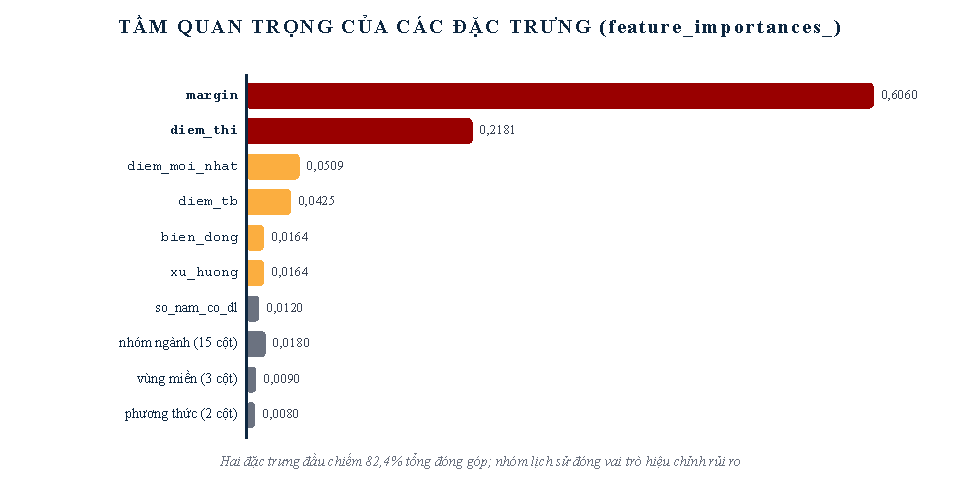
\includegraphics[width=0.92\textwidth]{figs/svg/h-feature-importance.pdf}
\caption{Mức đóng góp của toàn bộ các nhóm đặc trưng trong mô hình Random Forest.}
\label{fig:feature-importance}
\end{figure}

Hình~\ref{fig:feature-importance} cho thấy một điểm mà Bảng~\ref{tab:fi} không thể
hiện: 20 cột one-hot (15 nhóm ngành, 3 vùng miền, 2 phương thức) cộng lại chỉ chiếm
khoảng 3,5\% mức đóng góp, thấp hơn cả \code{diem\_tb}. Kết quả này không có nghĩa
các cột đó vô dụng --- chúng vẫn cần thiết để mô hình phân biệt ngành có cùng
\code{margin} --- mà cho thấy thông tin phân loại chủ yếu đóng vai trò điều chỉnh biên
chứ không quyết định xu hướng chính. Đây cũng là lý do vì sao việc tăng số chiều từ 10
lên 27 không làm mô hình kém đi: chi phí thêm 17 cột one-hot là rất nhỏ so với lượng
thông tin mà hai đặc trưng số trung tâm mang lại.

\section{So sánh với các công cụ tra cứu hiện có}

Để thấy rõ vị trí của Uni Connect, Bảng~\ref{tab:so-sanh-congcu} đối chiếu bảy nhóm
chức năng của hệ thống với ba nhóm công cụ mà thí sinh thường dùng: cổng thông tin
tuyển sinh của trường, các trang báo tổng hợp điểm chuẩn và các ứng dụng tư vấn có
thu phí. Việc so sánh chỉ dựa trên chức năng quan sát được, không dựa trên số liệu
người dùng của các bên.

\begin{table}[H]
\centering
\caption{Đối chiếu chức năng giữa Uni Connect và các nhóm công cụ tra cứu hiện có.}
\label{tab:so-sanh-congcu}
\small
\begin{tabularx}{\textwidth}{@{}>{\raggedright\arraybackslash}p{4.1cm}
  >{\centering\arraybackslash}p{1.9cm}
  >{\centering\arraybackslash}p{2.1cm}
  >{\centering\arraybackslash}p{1.9cm}
  >{\centering\arraybackslash}p{1.6cm}@{}}
\toprule
\rowcolor{gray100}\bfseries\color{daunavy}Chức năng &
\bfseries\color{daunavy}Cổng trường &
\bfseries\color{daunavy}Trang tổng hợp &
\bfseries\color{daunavy}Ứng dụng tư vấn &
\bfseries\color{daumaroon}Uni Connect \\
\midrule
Tra cứu điểm chuẩn nhiều năm & Một trường & Có & Có & Có \\
Gom dữ liệu toàn quốc một chỗ & Không & Một phần & Một phần & Có \\
Xác suất trúng tuyển theo hồ sơ & Không & Không & Có & Có \\
Phân tầng An toàn / Vừa sức / Thử sức & Không & Không & Một phần & Có \\
Lời giải thích kèm từng gợi ý & Không & Không & Không & Có \\
Lưu hồ sơ và lịch sử gợi ý & Không & Không & Có & Có \\
Cập nhật dữ liệu năm mới, huấn luyện lại & Không & Không & Không & Có \\
Mã nguồn mở, tự vận hành & Không & Không & Không & Có \\
\bottomrule
\end{tabularx}
\end{table}

Bảng~\ref{tab:so-sanh-congcu} cho thấy không nhóm công cụ nào có đủ cả bốn đặc điểm
mà đồ án hướng tới: dữ liệu gom một chỗ, xác suất tính theo hồ sơ cá nhân, phân tầng
kèm lời giải thích và khả năng tự cập nhật dữ liệu. Cổng thông tin của từng trường có
dữ liệu chính xác nhất nhưng chỉ phục vụ một trường và không có công cụ định lượng
rủi ro. Các trang tổng hợp giải quyết được bài toán tra cứu nhưng dừng ở việc hiển thị
bảng điểm thô. Ứng dụng tư vấn có thu phí tiến gần hơn ở khâu tính xác suất, nhưng
phần giải thích thường là câu văn cố định và người dùng không kiểm chứng được căn cứ.
Khoảng trống đó chính là lý do đồ án chọn hướng tiếp cận minh bạch: mọi con số dẫn
đến quyết định phân tầng đều hiển thị lại cho người dùng.

\section{Bàn luận}

Khoảng cách 2,42 điểm phần trăm Accuracy giữa hai mô hình nhỏ hơn khoảng cách ROC-AUC
(8,19 điểm), cho thấy lợi ích lớn nhất của Random Forest nằm ở chất lượng xếp hạng và
hiệu chuẩn xác suất chứ không chỉ nhãn cứng. Đây đúng là khía cạnh hệ thống cần nhất
vì quyết định phân tầng phụ thuộc toàn bộ vào thứ tự và giá trị $p$.

Phân tích ca sai cho thấy lỗi tập trung tại vùng \code{margin} gần 0 (từ $-0{,}5$ đến
$+0{,}5$): thí sinh ngang điểm chuẩn, nơi nhiễu tuyển sinh năm đơn lẻ (chỉ tiêu, phổ
điểm) át tín hiệu lịch sử. Đây là vùng hệ thống cố tình đẩy vào tầng Vừa sức kèm cảnh
báo biến động, thay vì khẳng định chắc chắn.

\section{Hạn chế}

\begin{itemize}[leftmargin=1.6em, itemsep=2pt]
  \item \textbf{Nhãn giả lập, không phải đỗ/trượt thật:} 11 mức \code{DELTAS} đối xứng chỉ xấp xỉ phân phối thí sinh; nhóm điểm xa chuẩn ($\pm 3{,}0$) dễ phân loại làm phồng Accuracy tổng thể.
  \item \textbf{Giới hạn hai phương thức:} Chưa xử lý đánh giá năng lực, đánh giá tư duy, chứng chỉ ngoại ngữ do khác thang điểm.
  \item \textbf{Nhiễu năm đơn lẻ:} Ngành mới mở, ngành đổi chỉ tiêu đột biến hoặc năm thiếu dữ liệu khiến \code{xu\_huong} và \code{bien\_dong} kém ổn định; hệ thống hiện gắn cờ ``dữ liệu mỏng'' thay vì dự báo mù.
  \item \textbf{Chưa kiểm thử tải đồng thời:} Đo 0,42 giây thực hiện trên truy vấn đơn; chưa đo tải hàng trăm người dùng song song mùa cao điểm.
\end{itemize}

\section{Tổng kết chương}

Chương này đã trình bày phần hiện thực và đo lường của đồ án: môi trường triển khai
với cấu hình tối thiểu 1 vCPU và 2~GB RAM, sáu bước của pipeline dữ liệu ngoại tuyến,
ba cấp độ kiểm thử với sáu ca chức năng đều đạt, và kết quả thực nghiệm của mô hình
trên tập kiểm thử độc lập năm 2025. Random Forest đạt Accuracy 74,56\%, ROC-AUC
0,8354 và Brier 0,1763, vượt mô hình đối chứng ở cả bốn chỉ số. Những hạn chế còn lại
--- chủ yếu là nhãn giả lập và phạm vi hai phương thức xét tuyển --- được tổng hợp ở
cuối chương và là cơ sở cho các hướng phát triển trình bày ở
Chương~\ref{ch:ketluan}.

\chapter{Kết luận và hướng phát triển}
\label{ch:ketluan}

\section{Kết luận}

Đồ án xây dựng thành công hệ thống gợi ý nguyện vọng đại học Uni Connect, khép kín từ thu thập dữ liệu 10 năm (2016--2025) đến triển khai web phục vụ người dùng. Kết quả chính:

\begin{itemize}[leftmargin=1.6em, itemsep=2pt]
  \item \textbf{Cơ sở dữ liệu thực tế quy mô lớn:} 295 trường, 3.037 ngành, 340 tổ hợp môn và 240.483 bản ghi điểm chuẩn qua 10 năm, giải quyết bài toán dữ liệu phân tán.
  \item \textbf{Mô hình học máy đáng tin cậy:} Random Forest với 27 đặc trưng đạt Accuracy 74,56\%, ROC-AUC 0,8354 và Brier score 0,1763 trên tập kiểm thử độc lập năm 2025, vượt trội so với Decision Tree cơ sở.
  \item \textbf{Gợi ý minh bạch có phân tầng:} Cơ chế 3 tầng (An toàn, Vừa sức, Thử sức) dựa trên xác suất trúng tuyển, kèm lời giải thích theo \code{margin}, \code{xu_huong} và \code{bien_dong}, giúp thí sinh xây dựng chiến lược nguyện vọng cân bằng.
  \item \textbf{Ứng dụng web hoàn chỉnh:} Viết trên Django 5.2 kết hợp MySQL 8.0, thời gian phản hồi trang gợi ý đạt 0,42 giây (dưới ngưỡng 3 giây), có cơ chế dự phòng không gián đoạn khi thiếu mô hình AI.
\end{itemize}

\section{Bài học rút ra}

\begin{itemize}[leftmargin=1.6em, itemsep=2pt]
  \item \textbf{Chất lượng và cấu trúc dữ liệu quyết định phần lớn hiệu năng:} Phần lớn thời gian đồ án tập trung vào làm sạch tên ngành, ánh xạ nhóm ngành, đồng bộ thang điểm và thiết kế bảng \code{cua_so_nam}. Khâu này đóng góp nhiều hơn việc tinh chỉnh sâu các siêu tham số học máy.
  \item \textbf{Ranh giới rò rỉ dữ liệu trong bài toán thời gian:} Chia dữ liệu ngẫu nhiên (k-fold truyền thống) sẽ gây rò rỉ tương lai vào quá khứ, tạo kết quả ảo. Việc chia cứng theo thời gian (huấn luyện 2021--2024, kiểm thử 2025) và tính đặc trưng chỉ từ các năm trước đó là điều kiện tiên quyết để đánh giá đúng năng lực mô hình.
  \item \textbf{Độ bền hệ thống quan trọng hơn độ phức tạp thuật toán:} Thiết kế bộ nhớ đệm nạp mô hình vào RAM và cơ chế dự phòng tự động chuyển sang xếp hạng \code{margin} khi lỗi nạp giúp hệ thống không bao giờ trả về lỗi 500 cho người dùng.
\end{itemize}

\section{Hướng phát triển}

\begin{itemize}[leftmargin=1.6em, itemsep=2pt]
  \item \textbf{Mở rộng phương thức xét tuyển:} Tích hợp điểm thi Đánh giá năng lực (ĐHQG Hà Nội, ĐHQG TP.HCM) và Đánh giá tư duy (ĐH Bách Khoa Hà Nội) thông qua module chuẩn hóa thang điểm tương đương.
  \item \textbf{Thu thập dữ liệu trúng tuyển thật:} Hợp tác hoặc khảo sát thí sinh sau mỗi mùa tuyển sinh để thu thập nhãn đỗ/trượt thật, thay thế dần nhãn giả lập từ \code{DELTAS}.
  \item \textbf{Tối ưu hóa gợi ý tổ hợp môn:} Bổ sung thuật toán phân bổ thứ tự nguyện vọng theo lý thuyết trò chơi hoặc quy hoạch tuyến tính nhằm tối đa hóa xác suất trúng ít nhất một nguyện vọng ưu tiên.
  \item \textbf{Kiểm thử tải và triển khai đám mây:} Đo đạc tải đồng thời trên nền tảng đám mây với cơ chế tự động mở rộng để phục vụ lượng truy cập lớn trong những ngày công bố điểm thi THPT.
\end{itemize}



\backmatter

\cleardoublepage
\phantomsection
\addcontentsline{toc}{chapter}{Tài liệu tham khảo}
\bibliographystyle{plain}
\bibliography{refs}

\chapter{Phụ lục}
\markboth{Phụ lục}{}

\section*{A. Hướng dẫn cài đặt và chạy chương trình}
\phantomsection
\addcontentsline{toc}{section}{A. Hướng dẫn cài đặt và chạy chương trình}

Các bước dưới đây hướng dẫn thiết lập môi trường và khởi chạy hệ thống Uni Connect từ kho mã nguồn.

\begin{lstlisting}[language=bash, caption={Quy trình cài đặt cơ sở dữ liệu, huấn luyện và khởi chạy Uni Connect.}]
# 1. Clone kho ma nguon
git clone https://github.com/tann299/DAU-2026-2027-Uni-Map.git
cd DAU-2026-2027-Uni-Map

# 2. Tao moi truong ao Python va cai dat goi phu thuoc
python -m venv .venv
source .venv/bin/activate      # Tren Linux / macOS / Git Bash
# .venv\Scripts\activate       # Tren Windows CMD / PowerShell
pip install -r requirements.txt

# 3. Thiet lap CSDL MySQL va nap du lieu ban dau
# Tao CSDL uni_map tren MySQL 8.0, sau do nap schema va du lieu:
mysql -u root -p uni_map < db/schema.sql
python source/backend/manage.py migrate --run-syncdb

# 4. Sinh tap dac trung va huan luyen mo hinh AI
python source/backend/recommendation/ml/gen_dataset.py
python source/backend/recommendation/ml/train.py

# 5. Khoi chay may chu ung dung Django
python source/backend/manage.py runserver 0.0.0.0:8000
# Mo trinh duyet truy cap: http://localhost:8000
\end{lstlisting}

\section*{B. Bảng tự kiểm trước khi nộp}
\phantomsection
\addcontentsline{toc}{section}{B. Bảng tự kiểm trước khi nộp}

\begin{tukiem}
  \item Sản phẩm chạy được trên môi trường máy chủ cục bộ và hosting thực tế.
  \item Đã kiểm tra kịch bản gợi ý và cơ chế dự phòng không phát sinh lỗi 500.
  \item Mã nguồn được quản lý bằng Git với lịch sử commit ghi nhận tiến độ liên tục.
  \item Có tệp \code{README.md}, \code{requirements.txt} và tài liệu hướng dẫn cài đặt rõ ràng.
  \item Mọi hình vẽ, bảng biểu và danh sách mã nguồn đều có tiêu đề, nhãn tham chiếu và được giải thích trong thân văn bản.
  \item Mọi mục tiêu đặt ra ở Chương~\ref{ch:modau} đều được đối chiếu kết quả cụ thể ở Chương~\ref{ch:caidat} và Chương~\ref{ch:ketluan}.
  \item Các con số thống kê dữ liệu (295 trường, 3.037 ngành, 240.483 bản ghi) và chỉ số mô hình (Accuracy 74,56\%, ROC-AUC 0,8354) lấy từ kết quả thực nghiệm thật.
  \item Mọi tài liệu tham khảo trong \code{refs.bib} đều được trích dẫn hợp lệ.
  \item Đã loại bỏ hoàn toàn các khung gợi ý, khung nội dung mẫu và dòng chữ ``NỘI DUNG MẪU'' trong tệp PDF.
\end{tukiem}

\section*{C. Nhận xét của giảng viên hướng dẫn}
\phantomsection
\addcontentsline{toc}{section}{C. Nhận xét của giảng viên hướng dẫn}

\khungnhanxet[7.5cm]

\vspace{0.8em}
\noindent\begin{minipage}[t]{0.5\textwidth}
\color{daunavy}
{\color{daumaroon}\bfseries Điểm số}

\vspace{0.7em}
\dongchamnhan{Bằng số:}

\vspace{0.9em}
\dongchamnhan{Bằng chữ:}
\end{minipage}\hfill
\okyten{\dauGVHD}{Giảng viên hướng dẫn}


\end{document}
